%%%%%%%%%%%%%%%%%%%%%%%%%%%%%%%%%%%%%%%%%%  不使用 authblk 包制作标题  %%%%%%%%%%%%%%%%%%%%%%%%%%%%%%%%%%%%%%%%%%%%%%
%-------------------------------PPT Title-------------------------------------
\title{{\rm VASP}算例举要}
%-----------------------------------------------------------------------------
%----------------------------Author & Date------------------------------------

%\author[\textrm{Jun\_Jiang}]{姜\;\;骏\inst{}} %[]{} (optional, use only with lots of authors)
%% - Give the names in the same order as the appear in the paper.
%% - Use the \inst{?} command only if the authors have different
%%   affiliation.
\institute[BCC]{\inst{}%
%\institute[Gain~Strong]{\inst{}%
\vskip -20pt 北京市计算中心~云平台事业部~~姜骏}
%\vskip -20pt {\large 格致斯创~科技}}
\date[\today] % (optional, should be abbreviation of conference name)
{%	{\fontsize{6.2pt}{4.2pt}\selectfont{\textcolor{blue}{E-mail:~}\url{jiangjun@bcc.ac.cn}}}
\vskip 45 pt {\fontsize{8.2pt}{6.2pt}\selectfont{%清华大学\;\;物理系% 报告地点
	\vskip 5 pt \textrm{2023.11.23-24}}}
}

%% - Either use conference name or its abbreviation
%% - Not really information to the audience, more for people (including
%%   yourself) who are reading the slides onlin%%   yourself) who are reading the slides onlin%%   yourself) who are reading the slides onlineee
%%%%%%%%%%%%%%%%%%%%%%%%%%%%%%%%%%%%%%%%%%%%%%%%%%%%%%%%%%%%%%%%%%%%%%%%%%%%%%%%%%%%%%%%%%%%%%%%%%%%%%%%%%%%%%%%%%%%%

\subject{}
% This is only inserted into the PDF information catalog. Can be left
% out.
%\maketitle
\frame
{
%	\frametitle{\fontsize{9.5pt}{5.2pt}\selectfont{\textcolor{orange}{“高通量并发式材料计算算法与软件”年度检查}}}
\titlepage
}
%-----------------------------------------------------------------------------

%------------------------------------------------------------------------------列出全文 outline ---------------------------------------------------------------------------------
\section{原子/分子计算}\label{Sec:atom-Pt}
%真空中的孤立原子的基态能量是\textrm{VASP}中最简单的算例,通过学习金属\textrm{Pt}原子基态能量的计算,可以掌握典型的\textrm{VASP}的主体流程\footnote{在所有计算之前,请确认\textrm{VASP}软件已经正确安装。},了解体系基态能量最小化的基本算法,并熟悉基本的输入/输出文件的内容。此外,还可以了解如何在已完成计算的基础上,进行计算精度提升或完成后续计算等一系列处理方式。
%\subsection{输入文件}
\frame{
	\frametitle{输入文件}
\textrm{VASP}要求所有的计算都在指定的计算目录下进行%(比如针对当前的算例,可以建目录\textrm{Pt\_atom})。
\begin{itemize}
	\item 准备计算所必需的四个输入文件:~文件名必须是\textcolor{magenta}{\textrm{INCAR}}、\textcolor{magenta}{\textrm{KPOINTS}}、\textcolor{magenta}{\textrm{POSCAR}}和\textcolor{magenta}{\textrm{POTCAR}}
%前三个文件,既可以手动输入也可以通过修改其余计算中的对应文件得到;~\textrm{POTCAR}文件存储的是计算对象构成元素的原子数据,包括具体的原子分波、赝原子分波以及赝势和构造赝势使用的交换-相关泛函等信息。\textrm{VASP}开发组在发布软件时会一并提供全部元素的\textrm{POTCAR}。\footnote{由于历史的原因,习惯上将\textrm{POTCAR}称为赝势文件,但实际上\textrm{POTCAR}文件中包含的内容不仅是原子赝势,还包括原子价电子分波函数和赝分波函数,以及补偿电荷等和赝势、\textrm{PAW}势相关的诸多信息,因此称“数据集(\textrm{Dataset})”更准确.}
	\item \textrm{INCAR}是\textrm{VASP}计算的核心控制文件
\end{itemize}
%\subsubsection{\rm{INCAR}}
对于\textrm{Pt}的计算,\textrm{INCAR}的设置:%如图\ref{Pt_atom:INCAR}所示。
\begin{figure}[h!]
\centering
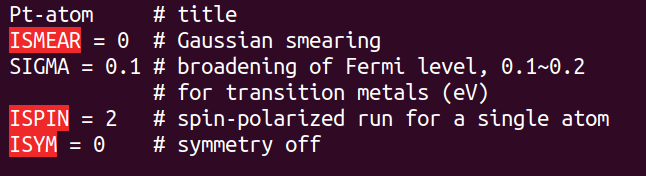
\includegraphics[height=1.00in,width=3.6in,viewport=0 0 480 135,clip]{Pt_atom-INCAR.png}
\caption{\fontsize{6.2pt}{5.2pt}\selectfont{\textrm{VASP}计算的主要输入控制文件\textrm{INCAR}.}}%(与文献\cite{EPJB33-47_2003}图1对比)
\label{Pt_atom:INCAR}
\end{figure}
对于原子/分子计算,只需要确定少量参数,其余的参数都采用软件推荐的默认值。
}

\frame
{
	\frametitle{\textrm{INCAR}参数}
计算设置的参数,说明如下:~
\begin{itemize}
	\item \textcolor{cyan}{\textit{ISMEAR}}:~设定\textrm{Fermi~}能级的展宽方法
		\vskip 5pt
		{\fontsize{7.2pt}{5.2pt}\selectfont{引入展宽为的是加速收敛
		%本例中参数确定的展宽方法是\textrm{Gaussian}展宽,该方法适用于单原子和局域体系,避免出现\textrm{Fermi}面附近占据数为负值
			。展宽值由参数\textcolor{cyan}{\textit{SIGMA}}确定}}
	\item \textcolor{cyan}{\textit{ISPIN}}:~因为\textrm{Pt}原子的价电子态是$5\mathit{d}^96\mathit{s}^1$,含有未成对电子,因此计算需要考虑自旋极化
	\vskip 5pt
	{\fontsize{7.2pt}{5.2pt}\selectfont{相比于非自旋极化的计算量加倍,即两种自旋(\textrm{spin-up/spin-down})下的电荷密度都要计算}}
	\item \textcolor{cyan}{\textit{ISYM}}:~控制对称性的计算参数%。本次计算中不考虑体系的点群对称性
\end{itemize}
}
%\subsubsection{\rm{KPOINTS}}
\frame
{
	\frametitle{\textrm{KPOINTS}参数}
\textrm{KPOINTS}是描述不可约\textrm{Brillouin}区(\textrm{Irreducible Brillouin Zone,~IBZ})的$\vec k$-点分布的文件%,见图\ref{Pt_atom:KPOINTS}。
\begin{figure}[h!]
\centering
\vskip -5pt
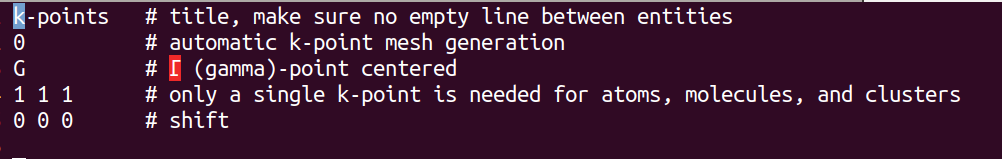
\includegraphics[height=0.60in,width=4.0in, viewport=0 20 750 118,clip]{Pt_atom-KPOINTS.png}
\caption{\fontsize{6.2pt}{5.2pt}\selectfont{\textrm{VASP}计算的\textrm{IBZ}中的$\vec k$点分布文件\textrm{KPOINTS}.}}%(与文献\cite{EPJB33-47_2003}图1对比)
\label{Pt_atom:KPOINTS}
\end{figure}
因为计算的是单原子体系,无需考虑\textrm{Bloch}定理的影响,因此只需要取一个$\vec k$点($\Gamma$点)
}
%\subsubsection{\rm{POSCAR}}
\frame
{
	\frametitle{\textrm{POSCAR}参数}
\textrm{POSCAR}是描述计算对象结构的文件%,见图\ref{Pt_atom:POSCAR}。
\begin{figure}[h!]
\centering
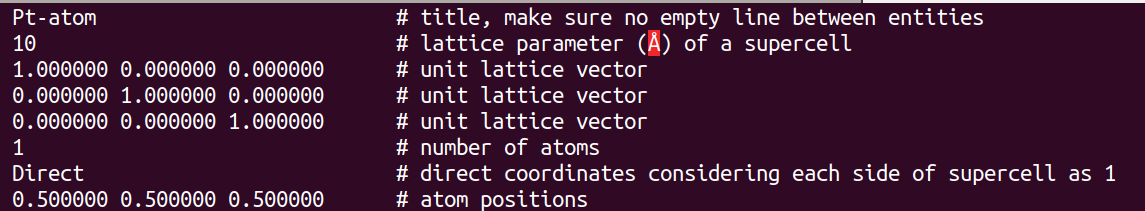
\includegraphics[height=0.95in,width=4.0in,viewport=0 0 850 155,clip]{Pt_atom-POSCAR.png}
\caption{\fontsize{6.2pt}{5.2pt}\selectfont{\textrm{VASP}计算对象的结构文件\textrm{POSCAR}.}}%(与文献\cite{EPJB33-47_2003}图1对比)
\label{Pt_atom:POSCAR}
\end{figure}
\textrm{VASP}中所有的计算对象必须是周期体系,因此对于单原子体系,可以将原子置于一个大的超晶胞($10\times10\times10$)中心,以此确保原子间相互作用足够小
}
%\subsubsection{\rm{POTCAR}}
\frame
{
	\frametitle{\textrm{POTCAR}参数}
%\textrm{POTCAR}是计算对象构成元素的数据集文件,包含了\textrm{PAW}计算所需的原子数据,见图\ref{Pt_atom:POTCAR}。本次计算使用\textrm{PAW\_PBE}数据集,是兼顾精度和效率的考虑。\textrm{POTCAR}文件可通过复制\textrm{VASP}提供的原子数据集库中的对应元素数据得到:\\
%\textcolor{magenta}{\textrm{cat~~potcar.PBE.paw/Pt/POTCAR~>~POTCAR}}\\
\begin{figure}[h!]
\centering
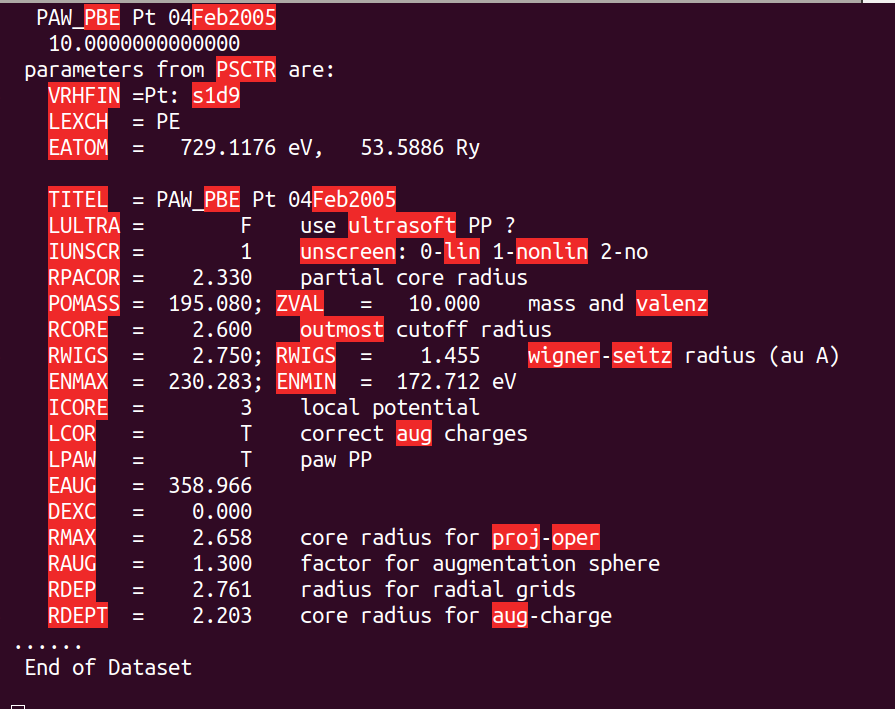
\includegraphics[height=2.7in,width=4.0in,viewport=0 15 780 528,clip]{Pt_atom-POTCAR.png}
\caption{\fontsize{6.2pt}{5.2pt}\selectfont{\textrm{VASP}计算的原子数据集文件\textrm{POTCAR}.}}%(与文献\cite{EPJB33-47_2003}图1对比)
\label{Pt_atom:POTCAR}
\end{figure}
%注意,这里参数\textit{ENMAX}的值230.283\textrm{eV}将作为计算中能量截断参数\textit{ENCUT}的默认值
}
%\subsection{VASP的运行}
%\textrm{VASP}软件安装在\textrm{Linux}系统环境下,因此在运行\textrm{VASP}的时候需要掌握\textrm{Linux}的一些基本命令。当上节中指定的四个输入文件准备完毕后,只要输入命令:\\
%\textcolor{magenta}{\textrm{VASP\_RUN\_PATH}}\footnote{假设\textrm{VASP}软件正确安装,\textcolor{magenta}{\textrm{VASP\_RUN\_PATH}}表示其可执行文件.}\\
%即可执行,随后屏幕上会有输出,直到计算结束。见图\ref{Pt_atom:runout}。
%\begin{figure}[h!]
%\centering
%%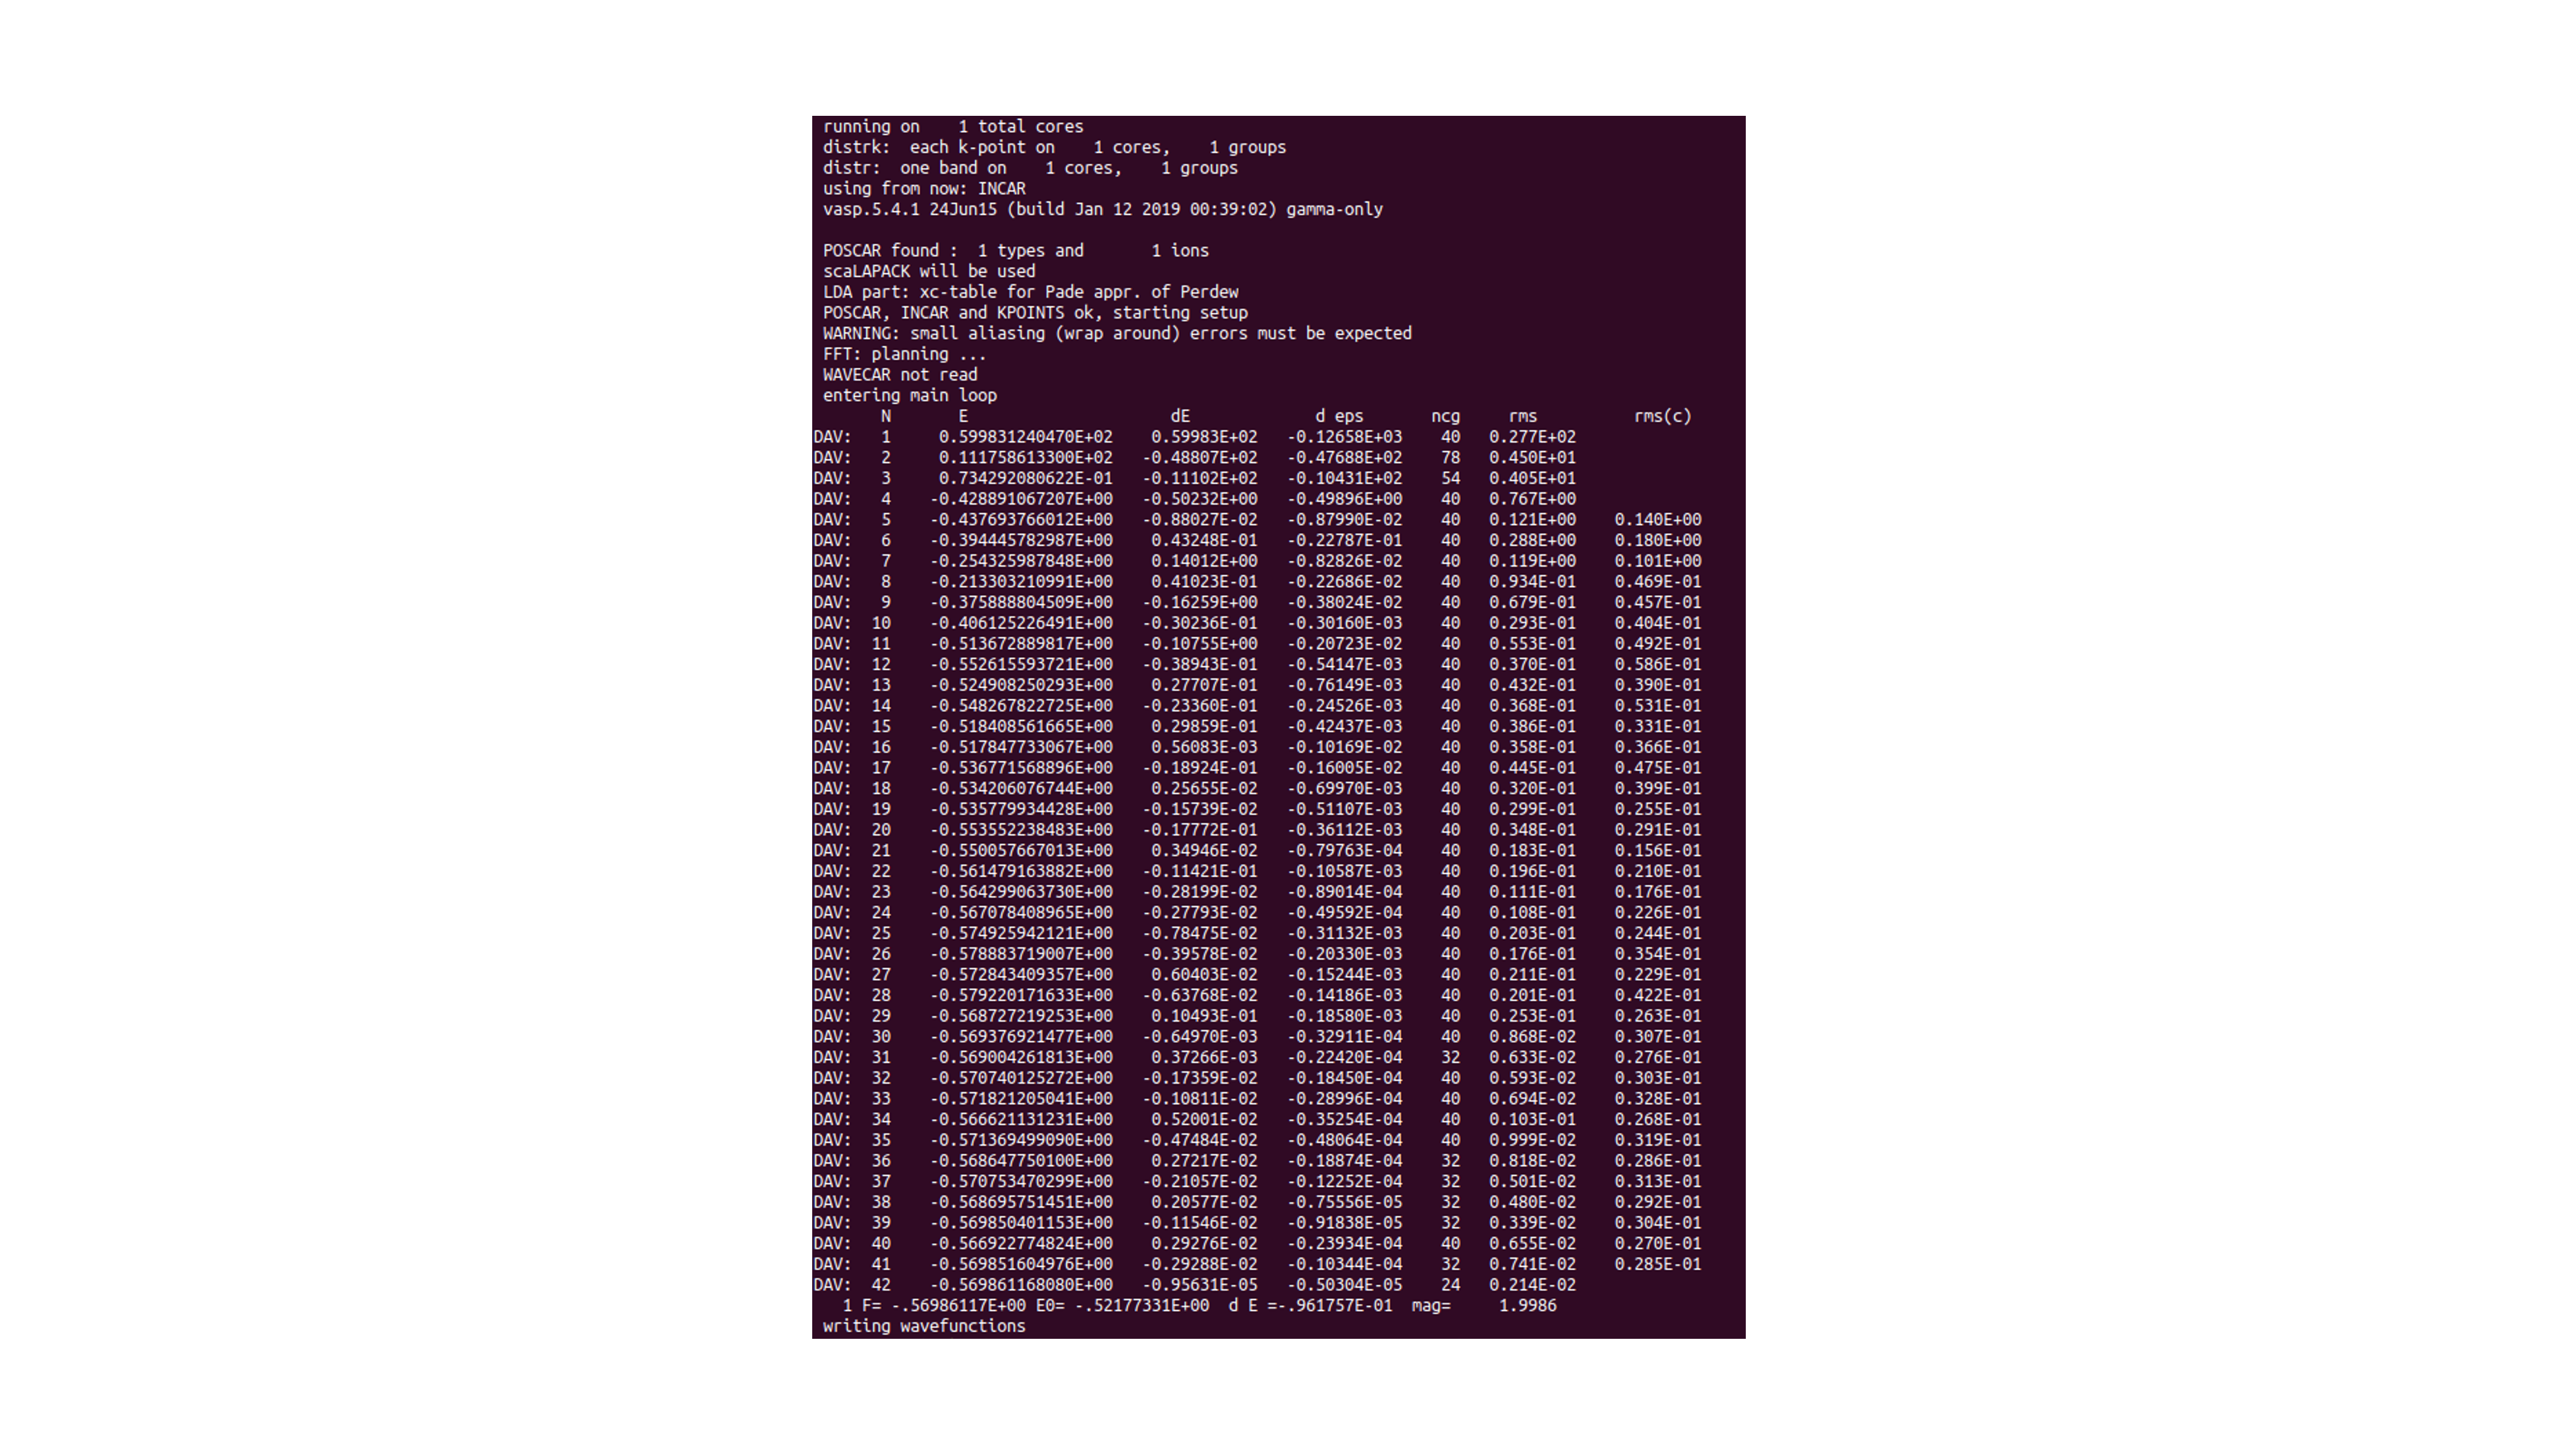
\includegraphics[height=4.5in,width=4.2in,viewport=0 0 780 530,clip]{Pt_atom-runout.png}
%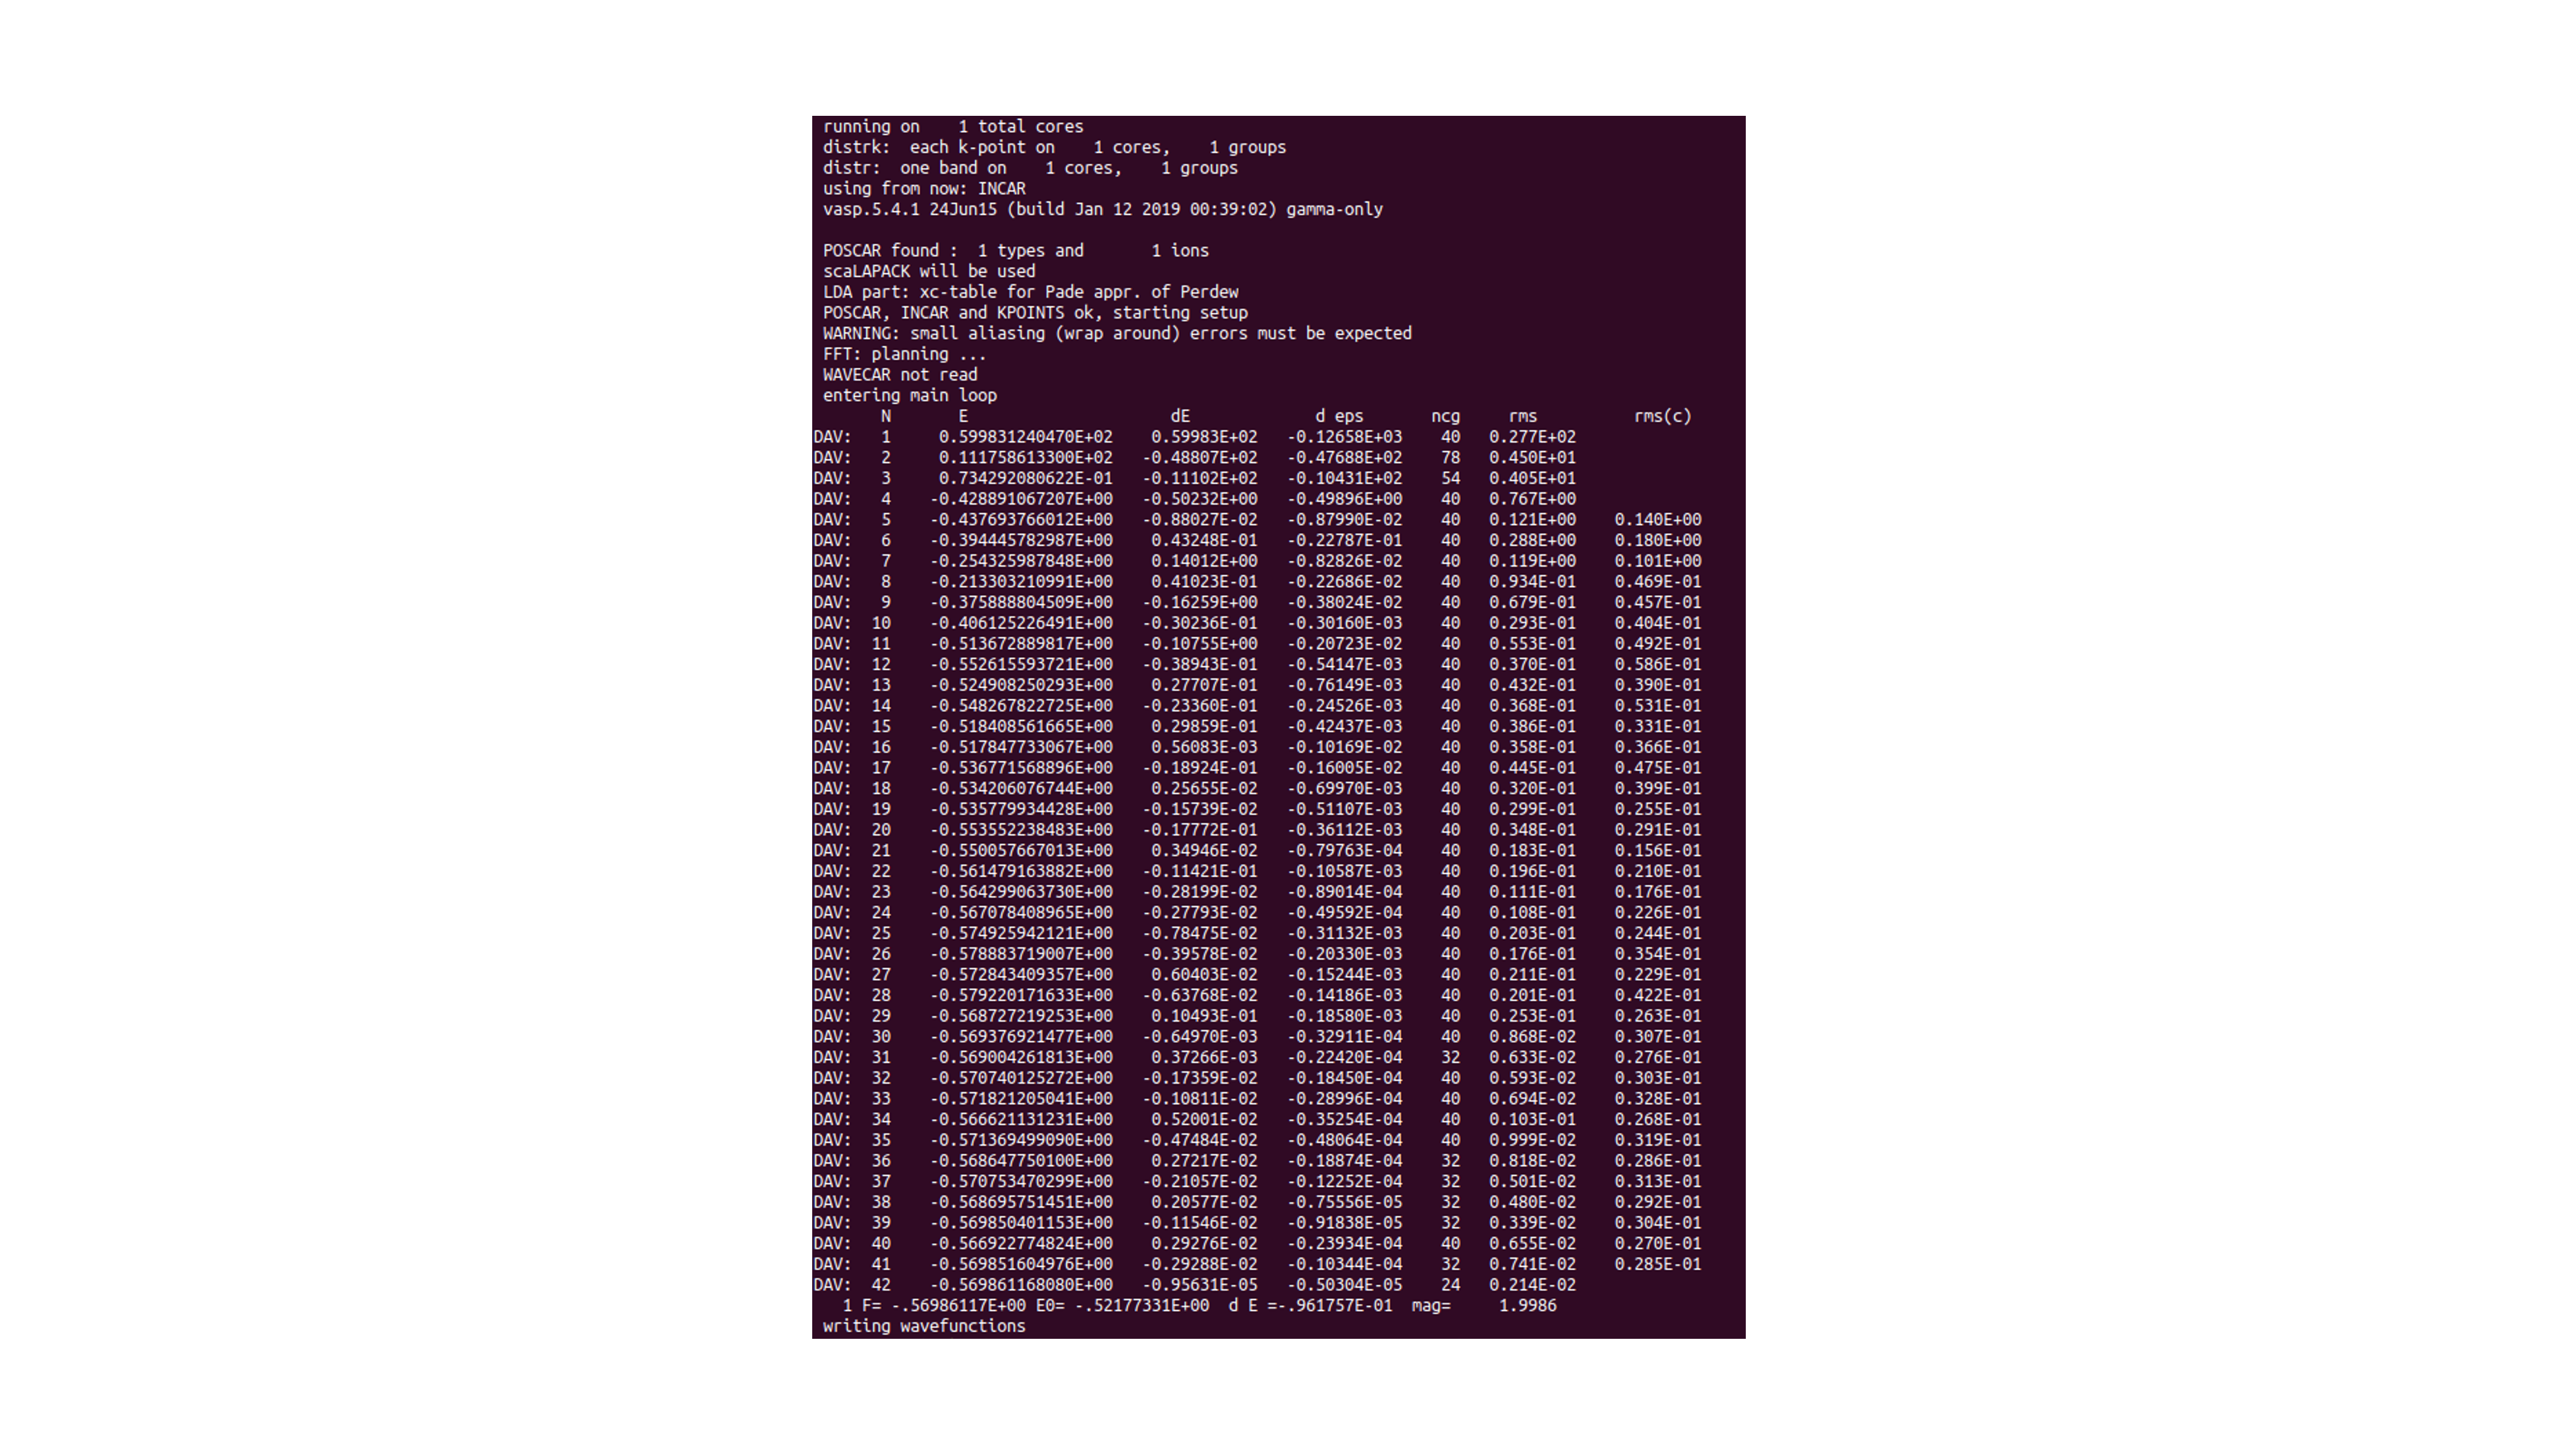
\includegraphics[width=5.9in,viewport=880 0 1870 1465,clip]{Pt_atom-runout.png}
%\caption{\small \textrm{VASP}运行时的屏幕输出.}%(与文献\cite{EPJB33-47_2003}图1对比)
%\label{Pt_atom:runout}
%\end{figure}
%从输出内容中可以看到警告提示\textrm{wrap around},只要是\textrm{VASP}软件认为用于\textrm{FFT}计算的网格不够密,就会出现该提示。该提示提示用户,由于\textrm{FFT}网格不够密集,会导致电荷密度在\textrm{FFT}处理时存在混叠误差\textrm{(aliasing error)}。如果想避免出现该提示,可以搜索输出文件\textrm{OUTCAR}中的参数\textit{NGX/NGY/NGZ}避免混叠误差的推荐值,并在\textrm{INCAR}文件中设定该参数。不过通常情况下此处警告提示可以忽略,因为混叠误差对结果的影响微乎其微。当看到最后一行输出\textrm{writing wavefunctions},就表明\textrm{VASP}正常结束。
%\newpage
%\subsection{\rm{VASP}的结果}
\frame
{
	\frametitle{输出文件}
正常结束的\textrm{VASP}计算,会产生13个输出文件%,见图\ref{Pt_atom:lsout}。
\begin{figure}[h!]
\centering
\vskip -2pt
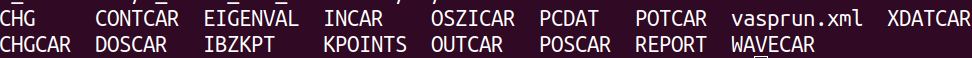
\includegraphics[height=0.20in,width=4.0in,viewport=0 2 750 38,clip]{Pt_atom-lsout.png}
\caption{\fontsize{6.2pt}{5.2pt}\selectfont{\textrm{VASP}运行结束后的文件.}}%(与文献\cite{EPJB33-47_2003}图1对比)
\label{Pt_atom:lsout}
\end{figure}

%以下先介绍\textrm{OSZICAR}和\textrm{OUTCAR}这两个文件。
%\subsubsection{\rm{OSZICAR}}
{\fontsize{7.5pt}{5.2pt}\selectfont{\textrm{OSZICAR}文件存储的是\textrm{VASP}迭代循环过程中的能量变化情况}}%,部分内容如图\ref{Pt_atom:OSZICAR}所示。
\begin{figure}[h!]
\centering
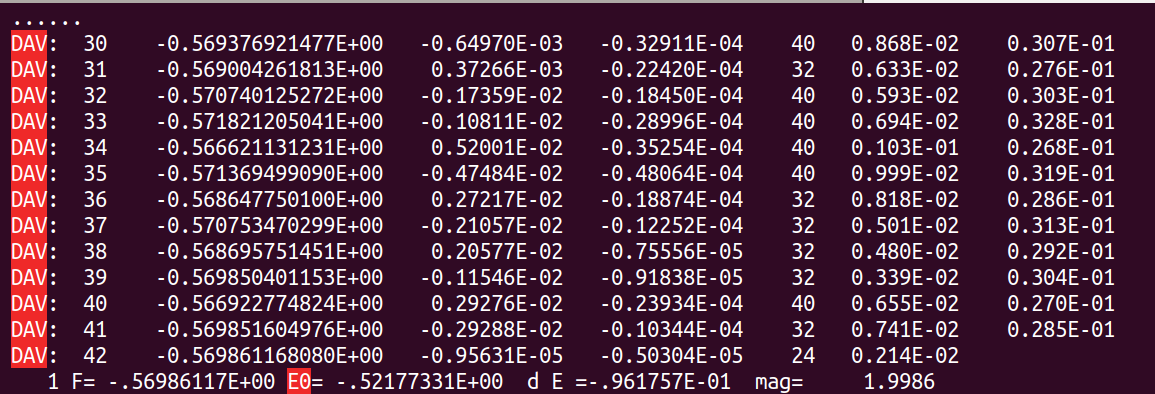
\includegraphics[height=1.2in,width=4.0in,viewport=0 0 880 290,clip]{Pt_atom-OSZICAR.png}
\caption{\fontsize{6.2pt}{5.2pt}\selectfont{\textrm{VASP}的输出文件\textrm{OSZICAR}(部分).}}%(与文献\cite{EPJB33-47_2003}图1对比)
\label{Pt_atom:OSZICAR}
\end{figure}
}

\frame
{
	\frametitle{\textrm{OSZICAR}}
	各列参数的含义
\begin{itemize}
	\item 第一列~~~:~表示矩阵迭代化的方法
	\item 第二列\textrm{N}:~统计两个离子步计算间的电子步迭代次数
	\item 第三列\textrm{E}:~当前的基态总能
	\item 第三列\textrm{dE}:~两次电子步迭代之间的基态总能变化
	\item 第四列\textrm{d~eps}:~两次电子步迭代的能量本征值的改变%(势保持不变)
	\item 第五列\textrm{ncg}:~完成一次迭代时,\textrm{Hamiltonian}算符\textbf{H}作用于轨道的次数~
	\item 第六列\textrm{rms}:~每次迭代开始时全部占据轨道的初始残矢\textrm{(residual vector)}——$\mathbf{R}=(\mathbf{H}-\varepsilon)\mathbf{S}|\phi\rangle$——之和\\{\fontsize{7.0pt}{5.2pt}\selectfont{该值表明轨道的收敛情形的优劣}}
	\item 第七列\textrm{rms(c)}:~一次迭代前后的电荷密度差
\end{itemize}
}

\frame
{
	\frametitle{\textrm{OSZICAR}}
%\textrm{OSZICAR}的第一列表示计算采用\textrm{Davidson}迭代收敛方法\\第二列为迭代次数%,本算例达到默认的收敛条件($\delta\mathrm{E}<1.0\times10^{-4}~\mathrm{eV}$)共迭代了42次。需要指出的是,
\textrm{Pt}的原子构型为([\textrm{Xe}]$4\mathit{f}^{14}5\mathit{d}^96\mathit{s}^1$)
\vskip 5pt
最后一行$\mathrm{E}_0$的值($-0.522\mathrm{eV}$)就是当前参数设置下,单个\textrm{Pt}原子在真空中的基态能量
{\fontsize{8.5pt}{5.2pt}\selectfont{
\begin{itemize}
	\item $\mathrm{E}_0$不是原子的绝对能量,而是\textrm{Pt}原子相对于\textrm{PAW}势的能量
\end{itemize}}}	
$\mathrm{mag}$的值($1.9986\mu_{\mathrm{B}}$)表示自旋极化计算的原子磁矩%(\textrm{Bohr magneton})
{\fontsize{8.5pt}{5.2pt}\selectfont{
\begin{itemize}
	\item 磁矩来自原子中两个未成对电子:
\begin{displaymath}
	\mathrm{mag}=\mu_{\mathrm{B}}[\rho_{\uparrow}-\rho_{\downarrow}]
\end{displaymath}
\end{itemize}}}
}
%\subsubsection{\rm{OUTCAR}}
\frame
{
	\frametitle{\textrm{OUTCAR}}
	\textcolor{red}{
\textbf{OUTCAR文件是\textrm{VASP}运行过程中最重要的输出文件}%,
}
%\textrm{OUTCAR}保存的是\textrm{VASP}运行中最详尽的过程记录:~

{\fontsize{7.5pt}{5.2pt}\selectfont{文件不仅包括输入文件的既有信息,还有计算体系的对称性分析,$\vec k$空间布点和具体位置,平面波基信息和最近邻原子的距离等基本信息;~此外记录了每一步离子弛豫和电子弛豫的计算信息}}%所以

\textrm{OUTCAR}的文件结构为:~
\begin{itemize}
	\item \textrm{VASP}版本和基本计算环境和计算资源信息
	\item 读入\textrm{INCAR}、\textrm{POTCAR}、\textrm{POSCAR}
	\item 最近邻原子和对称性分析信息
	\item 关于计算过程的详尽的控制参数信息(含默认值)
	\item 晶格正空间和$\vec k$-空间信息与原子坐标
	\item 平面波基信息(截断能和平面波数目)
	\item 非局域赝势信息
	\item 每个电子步计算的信息
	\end{itemize}
}

\frame
{
	\frametitle{\textrm{OUTCAR}}
	\begin{itemize}
		\item 每个电子步迭代的时间和能量信息
	\end{itemize}
\begin{figure}[h!]
\centering
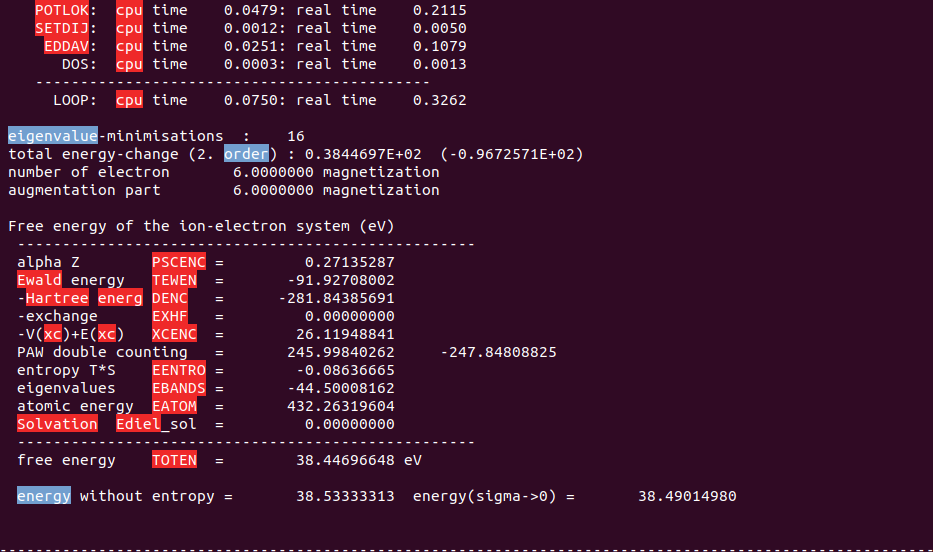
\includegraphics[height=2.5in,viewport=0 40 770 555,clip]{VASP_train-OUTCAR-iteration.png}
\caption{\fontsize{6.2pt}{5.2pt}\selectfont{\textrm{VASP}的输出文件\textrm{OUTCAR}的电子步迭代信息示例.}}%(与文献\cite{EPJB33-47_2003}图1对比)
\label{VASP_train-OUTCAR-iteration}
\end{figure} 
}

\frame
{
	\frametitle{\textrm{OUTCAR}}
	\begin{itemize}
	\item 能量本征值信息
	\end{itemize}
\begin{figure}[h!]
\centering
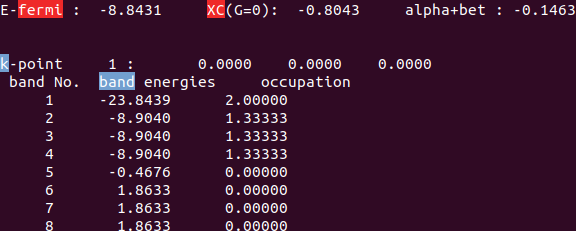
\includegraphics[height=1.5in,viewport=0 0 580 235,clip]{VASP_train-OUTCAR-eigenvalue.png}
\caption{\fontsize{6.2pt}{5.2pt}\selectfont{\textrm{VASP}的输出文件\textrm{OUTCAR}电子步迭代完成能量本征值信息示例.}}%(与文献\cite{EPJB33-47_2003}图1对比)
\label{VASP_train-OUTCAR-eigenvalue}
\end{figure}
}

\frame
{
	\frametitle{\textrm{OUTCAR}}
	\begin{itemize}
	\item 原子的受力与应力张量和晶胞信息
	\end{itemize}
\begin{figure}[h!]
\centering
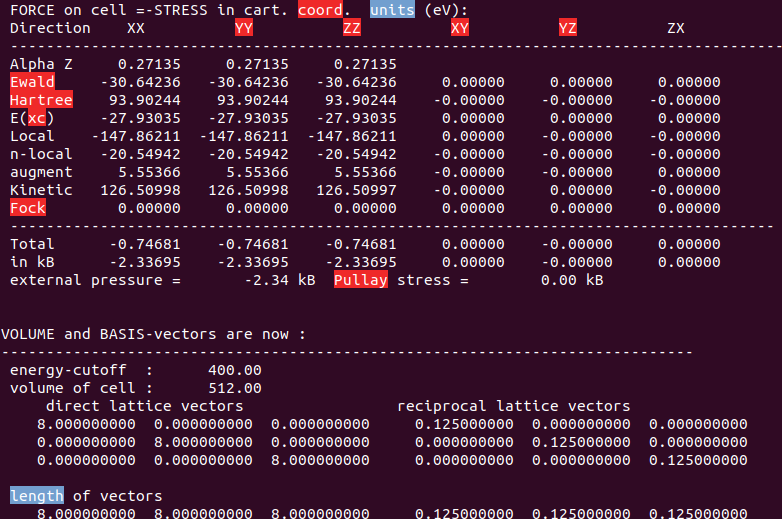
\includegraphics[height=2.5in,viewport=0 0 780 515,clip]{VASP_train-OUTCAR-stress_and_volumn.png}
\caption{\fontsize{6.2pt}{5.2pt}\selectfont{\textrm{VASP}的输出文件\textrm{OUTCAR}原子受力与应力张量和晶胞信息示例.}}%(与文献\cite{EPJB33-47_2003}图1对比)
\label{VASP_train-OUTCAR-stress_and_volumn}
\end{figure}
}

\frame
{
	\frametitle{\textrm{OUTCAR}}
	\begin{itemize}
	\item 体系基态总能和自由能信息
	\end{itemize}
\begin{figure}[h!]
\centering
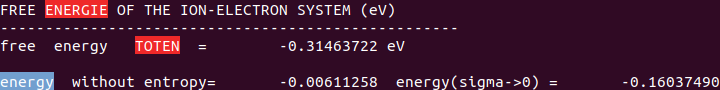
\includegraphics[height=0.5in,viewport=0 0 720 95,clip]{VASP_train-OUTCAR-free_energy.png}
\caption{\fontsize{6.2pt}{5.2pt}\selectfont{\textrm{VASP}的输出文件\textrm{OUTCAR}基态总能和自由能信息.}}%(与文献\cite{EPJB33-47_2003}图1对比)
\label{VASP_train-OUTCAR-free_energy}
\end{figure}
%}
%
%\frame
%{
%	\frametitle{\textrm{OUTCAR}}
%	\begin{itemize}
%	\item 完整计算过程的资源和计算时间统计信息
%\end{itemize}
%\begin{figure}[h!]
%\centering
%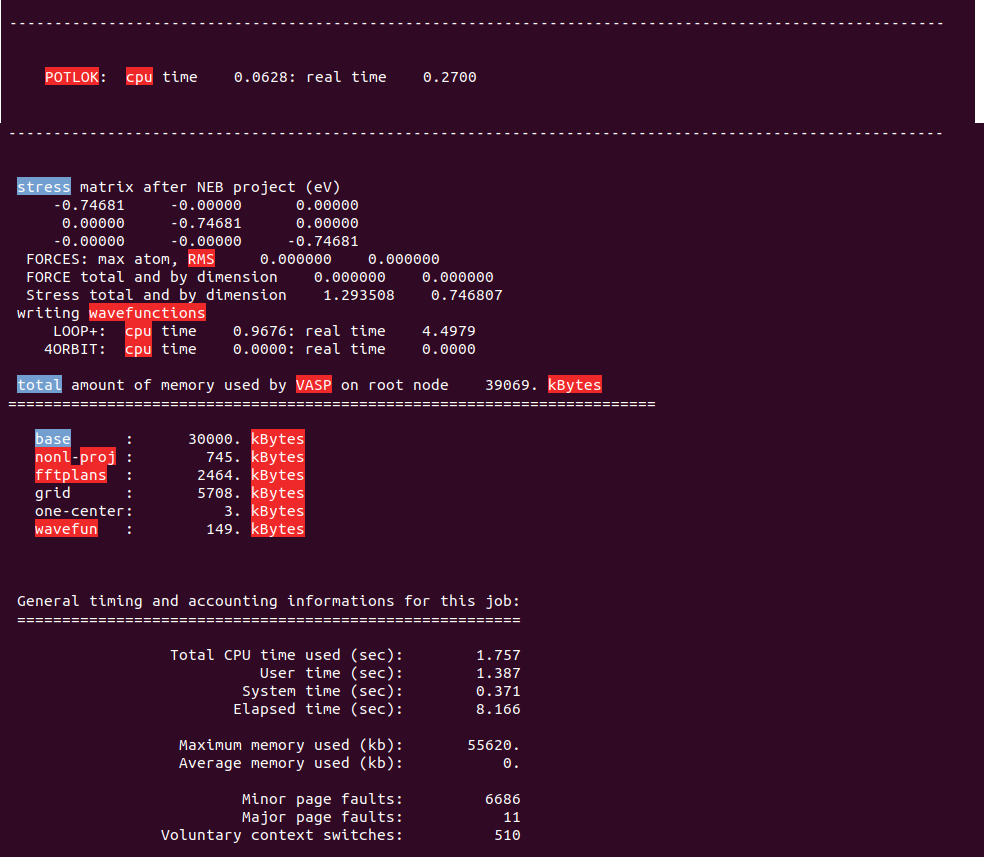
\includegraphics[height=2.7in,width=4.0in,viewport=5 0 680 835,clip]{VASP_train-OUTCAR-time_and_memory.png}
%\caption{\fontsize{6.2pt}{5.2pt}\selectfont{\textrm{VASP}的输出文件\textrm{OUTCAR}的计算资源和时间统计信息.}}%(与文献\cite{EPJB33-47_2003}图1对比)
%\label{VASP_train-OUTCAR-time_and_memory}
%\end{figure}
%}
% 在本算例中,
文件末尾记录的全部计算过程运行时间和计算资源使用情况%,如图\ref{Pt_atom:runtime}所示:
\begin{figure}[h!]
\centering
\vskip -2pt
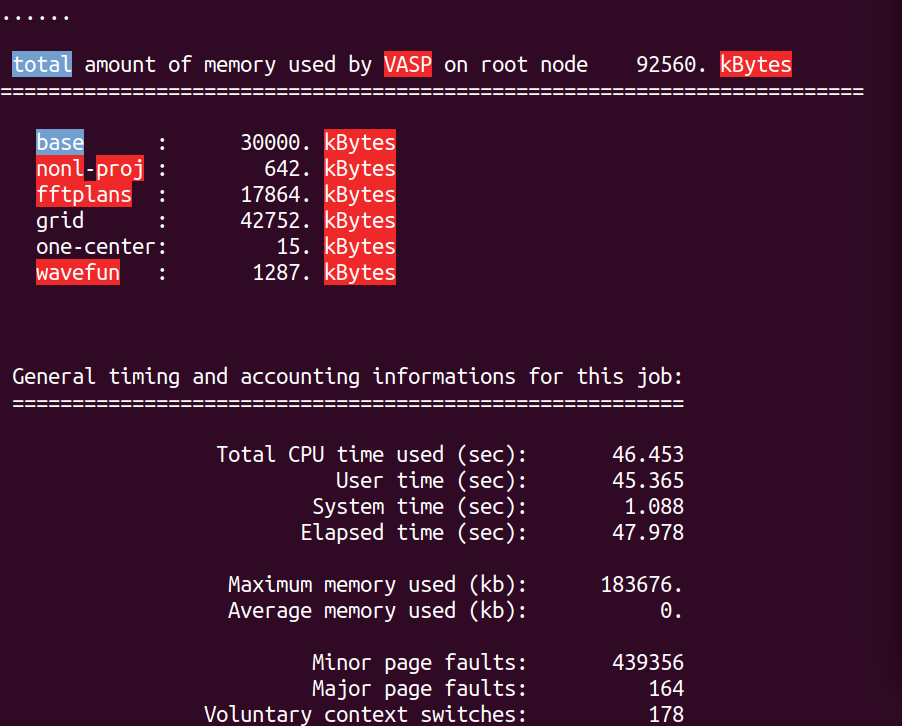
\includegraphics[height=1.2in,width=4.0in,viewport=0 0 680 215,clip]{Pt_atom-runtime.png}
\caption{\fontsize{6.2pt}{5.2pt}\selectfont{\textrm{VASP}的输出文件\textrm{OUTCAR}最后部分.}}%(与文献\cite{EPJB33-47_2003}图1对比)
\label{Pt_atom:runtime}
\end{figure}
%结果表明,\textrm{VASP}计算简单原子,只需要几十秒即可完成
}

\frame
{
	\frametitle{其余数据文件}
	除\textrm{OSZICAR}和\textrm{OUTCAR}外,还有三个重要的输出文件:~
	\begin{itemize}
		\item \textcolor{blue}{\textrm{CHGCAR}}:~存储体系的电荷密度
		\item \textcolor{blue}{\textrm{CONTCAR}}:~存储体系经结构弛豫后得到的原子位置和晶胞参数
		\item \textcolor{blue}{\textrm{WAVECAR}}:~存储体系最终的波函数文件(非格式输出的二进制文件)
	\end{itemize}
}

%\subsubsection{断点续算}
\frame
{
	\frametitle{断点续算}
\textrm{VASP}计算因故结束后,可以从中断计算位置继续完成计算,从而计算时间

执行断点续算的时候,除了需要将\textrm{CONTCAR}的内容复制到\textrm{POSCAR}中,还要对\textrm{INCAR}文件作必要的修改并增添如下内容:
\begin{figure}[h!]
\centering
\vskip -5pt
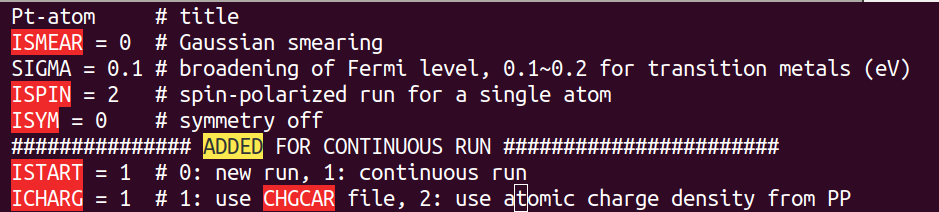
\includegraphics[height=1.0in,width=4.0in,viewport=0 0 700 157,clip]{Pt_atom-continurun.png}
\caption{\fontsize{6.2pt}{5.2pt}\selectfont{\textrm{VASP}断点续算的输入控制文件\textrm{INCAR}.}}%(与文献\cite{EPJB33-47_2003}图1对比)
\label{Pt_atom:continuruntime}
\end{figure}
再次运行\textrm{VASP},程序除了读取原来四个输入文件的内容,还将读取\textrm{CHGCAR}和\textrm{WAVECAR}的内容%,经过约近二十次迭代后,计算结果将进一步优化$\mathrm{E}_0=-.555\mathrm{~eV/atom}$,磁矩为$\mathrm{mag}=2.0000\mu_{\mathrm{B}}$,这次得到的原子基态能量将被用于后续体相\textrm{Pt}的结合能\textrm{(Cohesive energy)}计算。
}
\section{面心立方{\rm Pt}晶胞计算}\label{Sec:FCC-Pt}
%\subsubsection{\rm{POSCAR}}
\frame
{
	\frametitle{面心立方晶胞的结构}
	面心立方\textrm{(Face-centered Cubic, FCC)}结构的\textrm{Pt}晶体,晶胞参数为$a_0=3.975~\mathrm{\AA}$。每个面心立方中含有4个\textrm{Pt}原子
%面心立方\textrm{Pt}的晶胞中含有4个原子,在\textrm{POSCAR}文件中,四个原子分别置于原点和立方体的三个面心位置%。如图\ref{Pt_FCC:structure}所示。
\begin{figure}[h!]
\centering
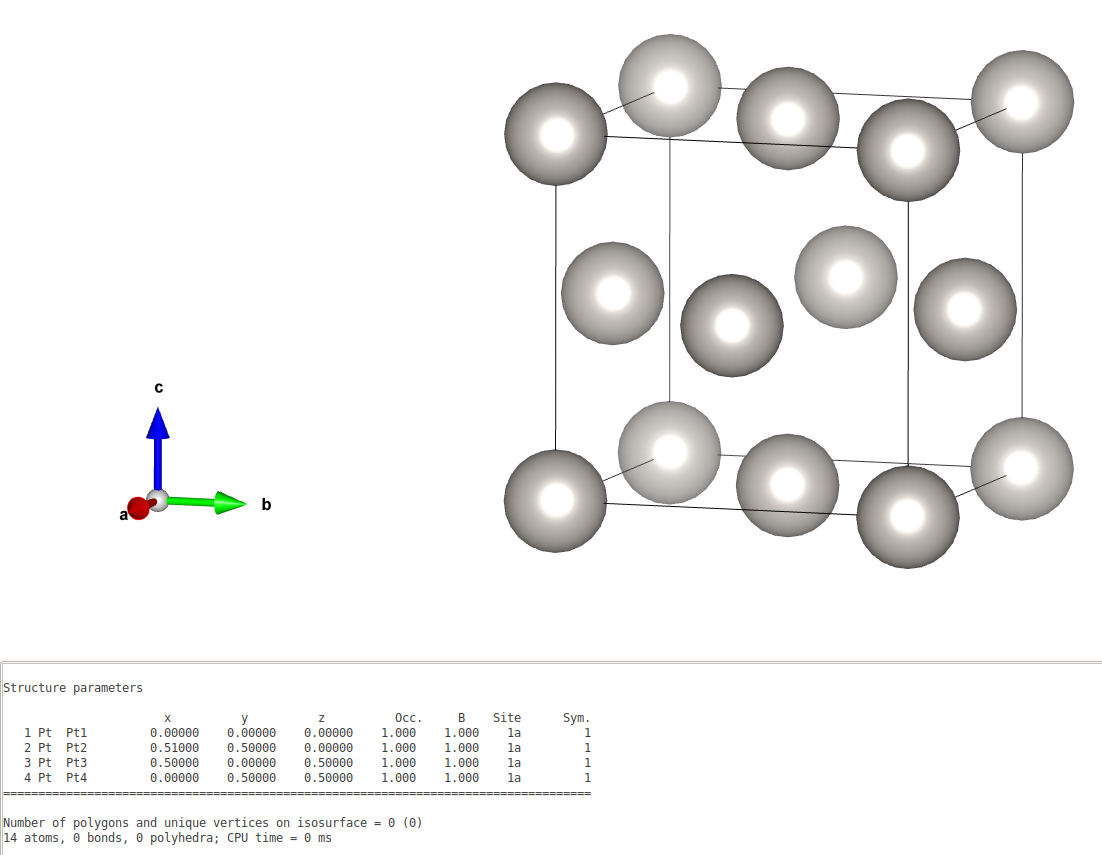
\includegraphics[height=1.8in,viewport=350 210 840 640,clip]{VASP_train-FCC.png}
\caption{\fontsize{6.2pt}{5.2pt}\selectfont{\textrm{FCC-Pt}的空间结构.}}%(与文献\cite{EPJB33-47_2003}图1对比)
\label{Pt_FCC:structure}
\end{figure}
}

\frame
{
	\frametitle{面心立方晶胞的\textrm{POSCAR}}
\begin{figure}[h!]
\centering
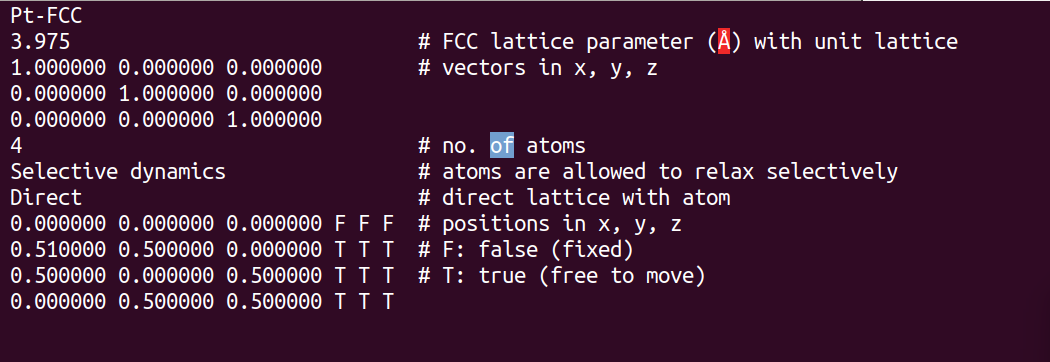
\includegraphics[height=1.5in,width=4.0in,viewport=0 30 740 270,clip]{Pt_FCC-POSCAR.png}
\caption{\fontsize{6.2pt}{5.2pt}\selectfont{用于\textrm{VASP}计算的\textrm{FCC-Pt}的结构文件\textrm{POSCAR}.}}%(与文献\cite{EPJB33-47_2003}图1对比)
\label{Pt_FCC:POSCAR}
\end{figure}
本算例中,晶胞中第一个\textrm{Pt}原子位置固定,其余三个原子允许在各个维度方向自由移动\\
{\fontsize{7.0pt}{5.2pt}\selectfont{注意到第二个\textrm{Pt}原子在$x$方向上偏移面心立方位置0.01%(见图\ref{Pt_FCC:POSCAR}),
结构弛豫时,如要求保持面心立方对称性,可以预见,经过结构弛豫后,晶胞将回到正常的面心立方位置}}
}

%\subsection{输入文件}
\frame
{
\frametitle{\textrm{INCAR}}
%这里计算的是
%计算\textrm{FCC-Pt},除了\textrm{POTCAR}与\textrm{Pt}原子相同,其余输入原子依次讨论如下:~
%\subsubsection{\rm{INCAR}}
%,计算中不再考虑自旋极化,输入文件\textrm{INCAR}如图\ref{Pt_FCC:INCAR}所示:
\begin{figure}[h!]
\centering
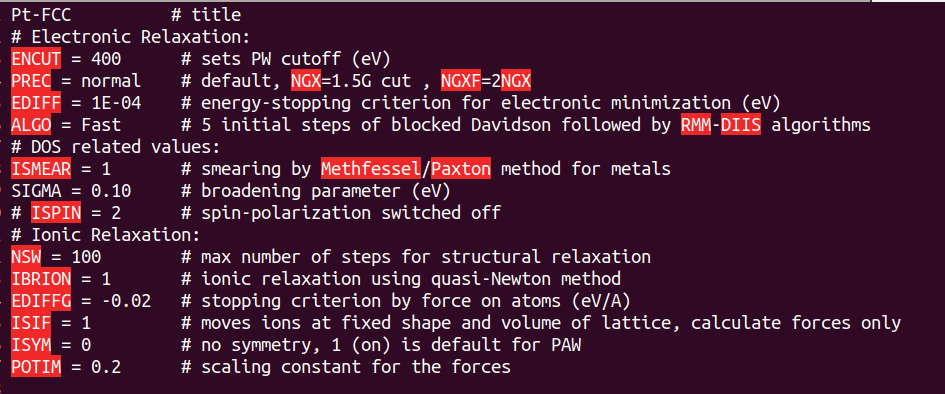
\includegraphics[width=4.0in,viewport=0 0 720 292,clip]{Pt_FCC-INCAR.png}
\caption{\fontsize{6.2pt}{5.2pt}\selectfont{\textrm{FCC-Pt}的输入控制文件\textrm{INCAR}.}}%(与文献\cite{EPJB33-47_2003}图1对比)
\label{Pt_FCC:INCAR}
\end{figure}
{\fontsize{7.2pt}{5.2pt}\selectfont{对含有偶数个相同原子的晶格,自旋电子密度趋于相同,忽略自旋部分贡献}}
}
%\begin{itemize}
%	\item \textit{ENCUT}:~该参数在需要手工指定平面波\textrm{(Plane Wave, PW)}基组截断能时使用,一旦该参数被指定,由参数\textit{PREC}确定的截断能不再有效。这里\textit{ENCUT}~=~400\textrm{~eV},远高于\textrm{POTCAR}中推荐的能量截断值(\textit{ENMAX}~=~230.283\textrm{~eV}),这样做主要是考虑到后续模拟\textrm{Pt}表面吸附\textrm{O}时,\textit{ENMAX}为400\textrm{~eV},计算组分体系时,平面波截断能应选为不低于最高的\textit{ENMAX}之值。
%	\item \textit{PREC}:~一旦人工指定\textit{ENCUT},参数\textit{PREC}确定的是波函数和电荷密度的\textrm{FFT}变换的网格精度,因此\textit{PREC}也是影响计算精度的参数。绝大多数情况下,参数值\textrm{``normal''}的精度足以满足要求;~如果有更高的精度要求,可以设为\textit{PREC}=\textrm{Accurate}。
%	\item \textit{EDIFF}:~该参数确定的是电子步迭代收敛的截断值,\textrm{VASP}计算中,要求最近邻两个电子步的总能(自由能)和\textrm{Kohn-Sham}方程能量本征值都满足收敛标准,程序才会停止运行。因此对一般计算来说,收敛标准的默认值$1.0\times10^{-4}$,已是足够的高精度。
%	\item \textit{ALGO}:~该参数确定的是离子步嵌套的电子步矩阵迭代对角化算法,参数值\textrm{``fast''}是最常用的,要求除了在第一个离子步弛豫时,最初五个电子步迭代采用稳定的\textrm{Davidson}算法,后续电子步迭代采用\textrm{RMM-DIIS}算法;~其余离子步弛豫,则只有第一个电子步弛豫采用\textrm{Davidson}算法,其余电子步都采用\textrm{RMM-DIIS}算法。
%	\item \textit{EDIFFG}:~该参数确定的是离子步弛豫的收敛截断值。当截断值为正,则要求最近邻两个离子步的总能(自由能)满足收敛标准;~当截断值为负,则要求计算对象中的每个原子上的受力都小于该值的绝对值(因此是更严格的收敛标准),默认值为$0.02\mathrm{eV/\AA}$。在没有达到收敛标准之前,程序将不断移动原子的位置;~在达到收敛标准之后,将不再改变体系中原子的位移。
%\end{itemize}
%对于一个新的\textrm{VASP}计算任务,初始波函数(也称为初猜波函数)可以通过原子赝势构造,这是符合物理直觉的。从不同截断能或不同结构的计算态出发,无疑将会节省计算时间。其余参数留待后续计算中说明。当需要对比两个体系的总能时,要确保两个体系的精度参数要求相同,这些参数包括:~\textit{ENCUT}、\textit{PREC}、\textit{EDIFF}、\textit{EDIFFG}和\textit{ISMEAR}。
%\subsubsection{\rm{KPOINTS}}
\frame
{
	\frametitle{\textrm{KPOINTS}}
$\vec k$空间布点数为$9\times9\times9$,布点方案由\textrm{Monkhorst-Pack}方法生成,这是对于金属和导体非常适用的布点方法%。如图\ref{Pt_FCC:KPOINTS}所示。
\begin{figure}[h!]
\centering
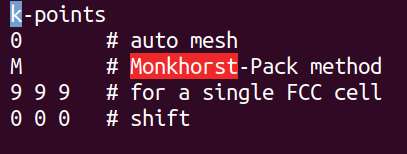
\includegraphics[width=4.0in,viewport=0 0 330 118,clip]{Pt_FCC-KPOINTS.png}
\caption{\fontsize{6.2pt}{5.2pt}\selectfont{\textrm{VASP}计算\textrm{FCC-Pt}的输入文件\textrm{KPOINTS}.}}%(与文献\cite{EPJB33-47_2003}图1对比)
\label{Pt_FCC:KPOINTS}
\end{figure}
}
%\subsection{用shell脚本运行VASP计算}
%\subsubsection{脚本运行}
%这里学习用\textrm{shell}脚本来提交\textrm{VASP}运行任务,后面的练习也将用脚本提交任务。提交\textrm{VASP}计算的\textrm{shell}脚本(文件名为\textcolor{green}{\textrm{run.vasp}})的内容如图\ref{Pt_FCC:run}所示:
%\begin{figure}[h!]
%\centering
%\vskip -12pt
%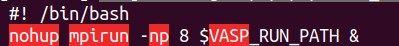
\includegraphics[height=0.3in,viewport=0 0 380 45,clip]{Pt_FCC-run.png}
%\caption{\small 提交\textrm{VASP}计算任务\textrm{FCC-Pt}的\textrm{shell}脚本内容.}%(与文献\cite{EPJB33-47_2003}图1对比)
%\label{Pt_FCC:run}
%\end{figure}
%	\begin{itemize}
%		\item 命令形式\textcolor{magenta}{~\textrm{nohup}~[执行命令]~\&~}表示将执行命令提交为后台进程,这样即使当前用户在计算执行过程中执行别的计算命令甚至退出,也不会影响计算任务正常的执行。这里\textrm{``nohup''}是\textrm{``no hang-up''}的缩写。
%		\item 命令中\textcolor{magenta}{\textrm{mpirun~-np~8~}}表示此次\textrm{VASP}计算用8个\textrm{CPU}并行完成。
%		\item \textcolor{magenta}{\$\textrm{VASP\_RUN\_PATH~}}表示\textrm{VASP}的执行文件的路径。
%	\end{itemize}
%将该执行脚本和\textrm{VASP}计算的四个输入文件放在同一个目录下,加可执行权限:~\\
%\textcolor{magenta}{chmod~+x~run.vasp}\\% \# change the file mode to execution mode\\
%然后就可以运行如下命令执行\textrm{VASP}计算:\\
%	\textcolor{magenta}{./run.vasp }\\
%		计算过程中,通过\textrm{Hellman-Feynman}定理计算作用在每个离子步位置上的原子受力,离子步迭代过程直到全部原子的受力都满足收敛标准\textit{EDIFFG}($0.02\mathrm{eV/\AA}$)。在计算过程中,可以通过以下命令监控原子受力情况的变化:\\
%		\textcolor{magenta}{grep~\`~drift~\'~ OUTCAR}
%\subsubsection{\rm{nohup.out}}
%用\textcolor{magenta}{$\mathrm{nohup}~[\cdots]~\&$}提交的任务,计算过程会保存在输出文件\textrm{nohup.out}中,如图\ref{Pt_FCC:nohupout}所示。
%%\newpage
%\begin{figure}[h!]
%\centering
%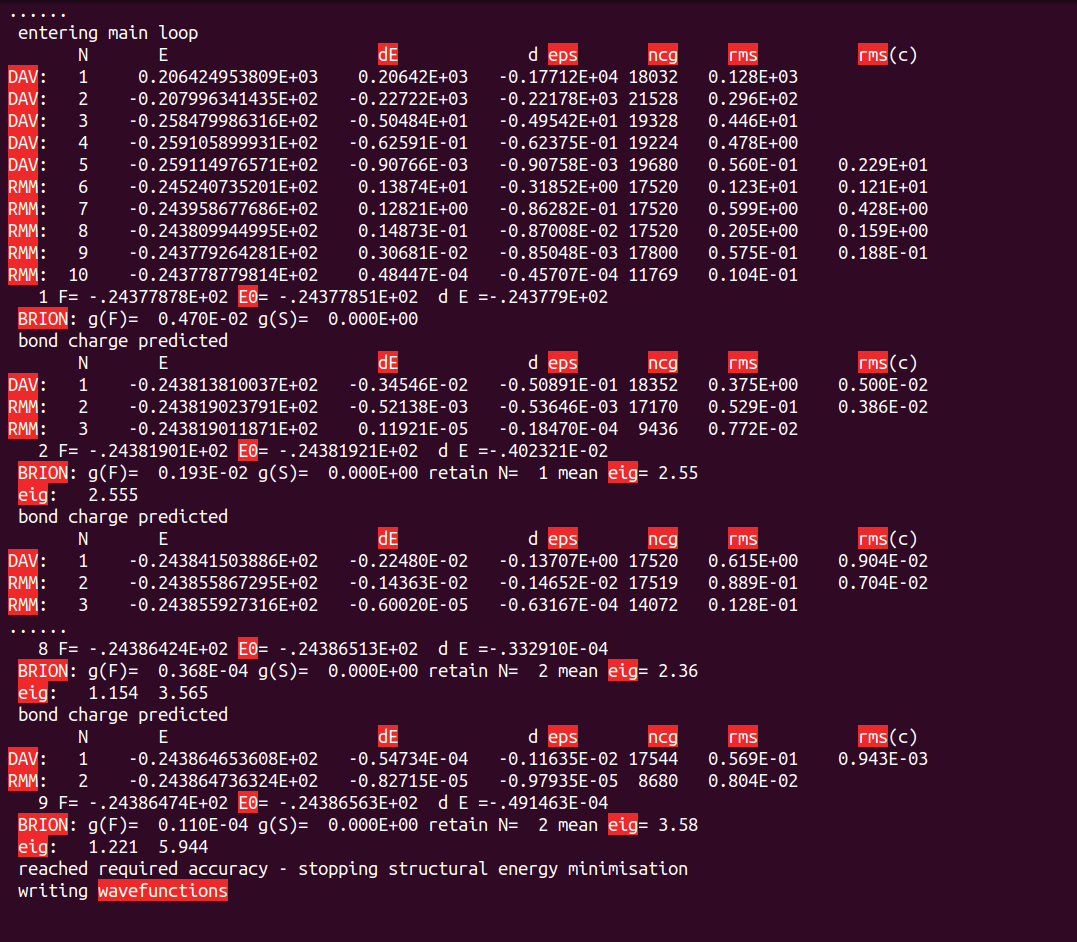
\includegraphics[height=5.5in,viewport=0 20 620 730,clip]{Pt_FCC-nohupout.png}
%\caption{\small \textrm{VASP}计算\textrm{FCC-Pt}的输出文件\textrm{nohup.out}.}%(与文献\cite{EPJB33-47_2003}图1对比)
%\label{Pt_FCC:nohupout}
%\end{figure}
%
%因为参数\textit{ALGO}=\textrm{fast},因此第一次离子步弛豫中,最初5步电子步迭代的矩阵对角化是\textrm{Davidson}方法,然后是\textrm{RMM-DIIS}方法;~电子步迭代结束后,根据原子受力,将原子移动到新的位置(完成离子弛豫),在新的原子构型下开始电子步迭代,循环往复,直到满足收敛标准(\textit{EDIFF}和\textit{EDIFFG})。最后出现的\textrm{``writing wave functions''}表明运行结束。波函数将写入\textrm{WAVECAR}文件中(参照\textrm{INCAR}中的输出设置)。
%\subsection{计算结果}
%\subsubsection{\rm{CONTCAR}与结构弛豫}
\frame
{
	\frametitle{结构弛豫:~\textrm{CONCAR}}
\textrm{CONTCAR}文件记录的是结构弛豫完成时晶体中原子的位置%,本算例\textrm{FCC-Pt}弛豫后的\textrm{CONTCAR}内容如图\ref{Pt_FCC:CONTCAR}所示。
\begin{figure}[h!]
\centering
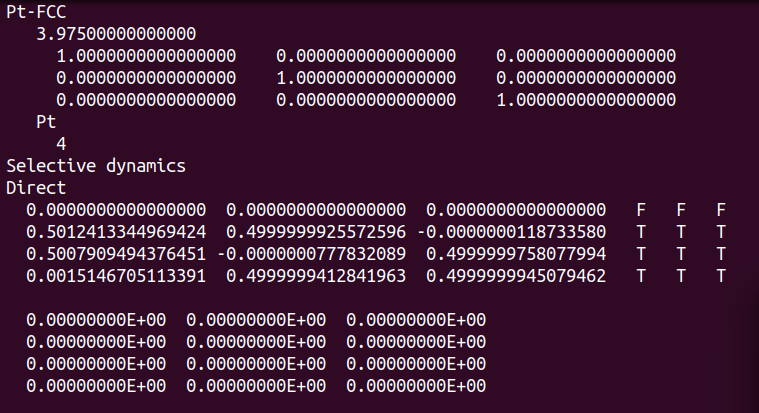
\includegraphics[width=4.0in,viewport=0 0 580 230,clip]{Pt_FCC-CONTCAR.png}
\caption{\fontsize{6.2pt}{5.2pt}\selectfont{\textrm{VASP}计算中记录\textrm{FCC-Pt}弛豫后结构的文件\textrm{CONTCAR}.}}%(与文献\cite{EPJB33-47_2003}图1对比)
\label{Pt_FCC:CONTCAR}
\end{figure}
{\fontsize{7.0pt}{5.2pt}\selectfont{显然,结构弛豫后,第二个原子由起始位置\textrm{(0.510000,~0.500000,~0.00000)}弛豫到\textrm{FCC}结构要求的原子位置(存在一定的数值误差)}}
}
\frame
{
	\frametitle{从\textrm{OUTCAR}中提取信息}
%\subsubsection{\rm{OUTCAR}}
%为监控
	离子步弛豫过程中体系总能量收敛情况%,可以使用以下命令检索输出文件\textrm{OUTCAR}:\\
%\textcolor{magenta}{\textrm{grep~~\'~energy~without~entropy~\'~~OUTCAR}}\\
%结果如图\ref{Pt_FCC:OUTCAR_totene}所示。
\begin{figure}[h!]
\centering
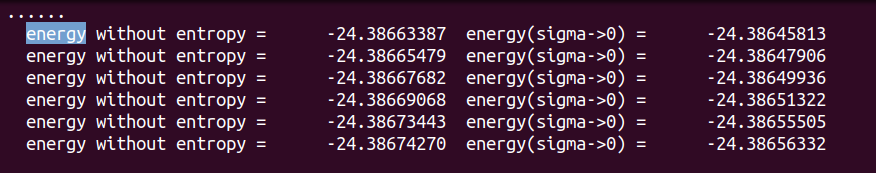
\includegraphics[width=4.0in,viewport=0 0 680 130,clip]{Pt_FCC-OUTCAR_totene.png}
\caption{\fontsize{6.2pt}{5.2pt}\selectfont{\textrm{VASP}计算\textrm{FCC-Pt}的弛豫过程的基态总能收敛情况.}}%(与文献\cite{EPJB33-47_2003}图1对比)
\label{Pt_FCC:OUTCAR_totene}
\end{figure}
{\fontsize{7.2pt}{5.2pt}\selectfont{离子步迭代收敛时的基态能量$\mathrm{E}_0$的值为~$-24.387\mathrm{~eV}$,换言之,当面心立方的晶胞参数为$3.975\mathrm{\AA}$时,体系中\textrm{Pt}原子的基态能量为$-24.387/4=-6.097\mathrm{eV/atom}$,比%\ref{Sec:atom-Pt}节计算的
孤立原子\textrm{Pt}的基态能量要低}}
}
%下一节我们将讨论晶胞参数的优化和影响\textrm{VASP}计算精度的重要参数的确定。
\section{收敛测试}\label{Sec:convergence}
\frame
{
	\frametitle{能量收敛测试}
对\textrm{DFT}迭代计算过程,随着迭代次数递增,体系总能(或自由能)会快速下降,随后进到逐渐平稳变化的区域,并伴随小的振荡,最终达到基态能量,%如图\ref{Fig:convergence}所示,
这个过程称为\textbf{收敛}。
\begin{figure}[h!]
	\vskip -5pt
\centering
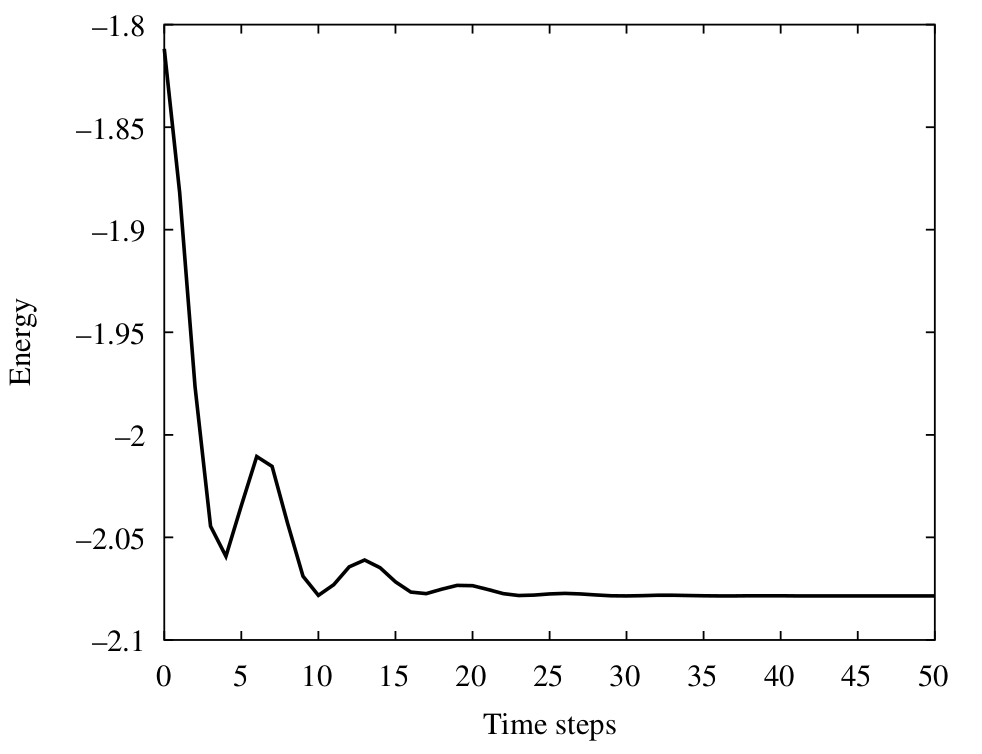
\includegraphics[width=3.0in,viewport=0 33 740 600,clip]{Ab-initio-Ene.png}
\caption{\fontsize{6.2pt}{5.2pt}\selectfont{迭代计算中的能量收敛示意图,引自文献\cite{Comp_Phys}.}}%(与文献\cite{EPJB33-47_2003}图1对比)
\label{Fig:convergence}
\end{figure}
{\fontsize{7.0pt}{5.2pt}\selectfont{对于任何研究体系,首先必须保证迭代计算能收敛,然后才谈得上进行有意义的\textrm{DFT}计算。同时,面对一个全新的计算体系,合理的收敛测试也是非常必要的,否则难免遭遇为克服迭代计算收敛的困难,浪费过多计算资源和精力}}
}

%考虑到\textrm{DFT}计算的本质是变分过程,因此只有各种初始条件选择都比较合理,计算才可能收敛到正确的结果,否则很可能收敛到错误的结果。在收敛测试中,最重要的参数主要包括:
%\begin{itemize}
%	\item \textrm{INCAR}中的参数\textit{ENCUT}
%	\item \textrm{KPOINTS}中的$\vec k$空间布点数目
%\end{itemize}
%在正常收敛测试中,两个参数的数值都应该由小到大逐渐增加,这将有助于考察计算体系的总能是否随参数逐渐趋于收敛。
%\subsection{能量收敛测试}
%体系截断能的定义
%\begin{equation}
%	E_{\mathrm{cut}}\geqslant\dfrac12|\vec k+\vec G|^2
%	\label{eq:Ecut}
%\end{equation}
%换句话说,截断能确定的是平面波基波矢的上限。一般截断能的取值范围是$150\sim400\mathrm{~eV}$,其默认阈值由计算体系组成元素的\textrm{POTCAR}中\textit{ENMAX}和\textit{ENMIN}中的极大值和极小值确定。但是,在具体计算过程中,合理的截断能应该通过测试确定。本次练习使用的\textrm{shell}脚本中,将包含3个输入文件(\textrm{INCAR},\textrm{KPOINTS}和\textrm{POSCAR})的设置,并且有4个不同的截断能参数\textit{ENCUT}(200,~225,~250和350\textrm{~eV})。计算中$\vec k$空间布点数固定($9\times9\times9$)。由此可以同时确定\textit{ENCUT}的收敛情况和平衡态晶胞参数。
%\subsubsection{\rm{shell}脚本\rm{run.lattice}}
%这里给出一个\textrm{shell}脚本的范例(文件名\textcolor{green}{\textrm{run.lattice}}),如图\ref{Pt_FCC-runlattice}所示,当前截断能为\textit{ENCUT}=250\textrm{~eV}。
%\begin{figure}[h!]
%\centering
%\hspace*{-20pt}
%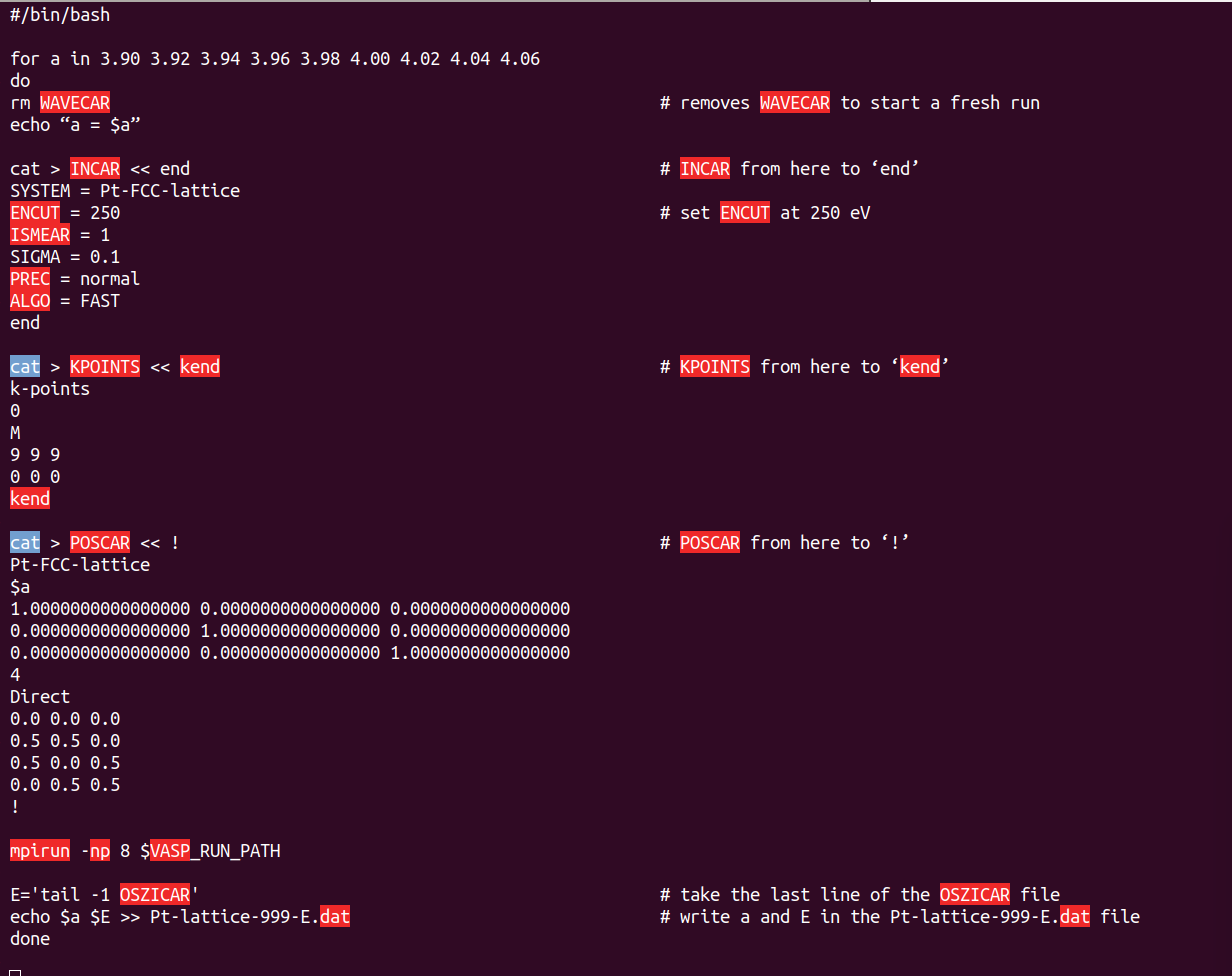
\includegraphics[height=5.2in,viewport=0 20 860 700,clip]{Pt_FCC-OUTCAR_runlattice.png}
%\caption{\small \textrm{FCC-Pt}截断能收敛测试\textrm{shell}脚本\textrm{run.lattice}示例.}%(与文献\cite{EPJB33-47_2003}图1对比)
%\label{Pt_FCC-runlattice}
%\end{figure}
%
%从该\textrm{shell}脚本内容看,晶胞参数将\textrm{\$a}从$3.90\mathrm{\AA}$到$4.06\mathrm{\AA}$变化,并且每改变一次晶胞参数将会执行一轮\textrm{VASP}晶格弛豫计算流程。因为是收敛测试,而平面波的收敛与自旋无关,因此\textrm{VASP}计算不考虑自旋极化的影响。
%
%有必要指出的是,在\textrm{shell}脚本中,生成\textrm{INCAR}、\textrm{KPOINTS}和\textrm{POSCAR}文件的各命令行必须连续,不能被注释或空行隔断,这一点请初学者务必注意。
%\subsubsection{\rm{测试脚本的执行}}
%与\ref{Sec:FCC-Pt}的\textrm{shell}脚本执行类似,首先可执行权限:\\
%\textcolor{magenta}{\textrm{
%chmod~+x~./run.lattice}}\\% \# change the file mode to execution mode\\
%再运行:\\
%\textcolor{magenta}{\textrm{./run.lattice }}
%\subsubsection{\rm{执行结果}}
%脚本执行完毕,结果将写入到文件\textrm{Pt-lattice-999-E.dat}中。因此当截断能\textit{ENCUT}=250\textrm{~eV}时,\textrm{FCC-Pt}的不同晶胞参数下得到不同的基态总能,可用命令\\
%\textcolor{magenta}{\textrm{cat~Pt-lattice-999-E.dat}}\\
%查看,如图\ref{Pt_FCC-energy-con}所示。
%\begin{figure}[h!]
%\centering
%\vskip -8pt
%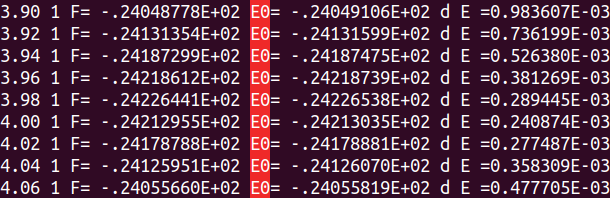
\includegraphics[height=1.3in,viewport=0 0 620 200,clip]{Pt_FCC-energy-con.png}
%\caption{\small \textrm{FCC-Pt}截断能收敛测试:~不同晶胞参数下的基态总能.}%(与文献\cite{EPJB33-47_2003}图1对比)
%\label{Pt_FCC-energy-con}
%\end{figure}
%
%图\ref{Pt_FCC-energy-curve}给出的是
%四种不同的截断能(分别是200,~225,~250和350\textrm{~eV})下的运行结果,截断能在\textit{ENCUT}=250\textrm{~eV}时,总能达到收敛(差别小于5\textrm{~meV})。平衡态的晶格参数为$3.077\mathrm{\AA}$,该值与\textrm{Bentmann}等的计算值$3.975\mathrm{\AA}$\cite{PRB78-205302_2008}吻合得很好,与实验值$3.928\mathrm{\AA}$\cite{Kittel}也较为接近。根据优化参数得到的体系总能为~--24.2269\textrm{~eV}(--6.057\textrm{~eV/atom})。
\frame
{
	\frametitle{截断能收敛测试}
\begin{figure}[h!]
\centering
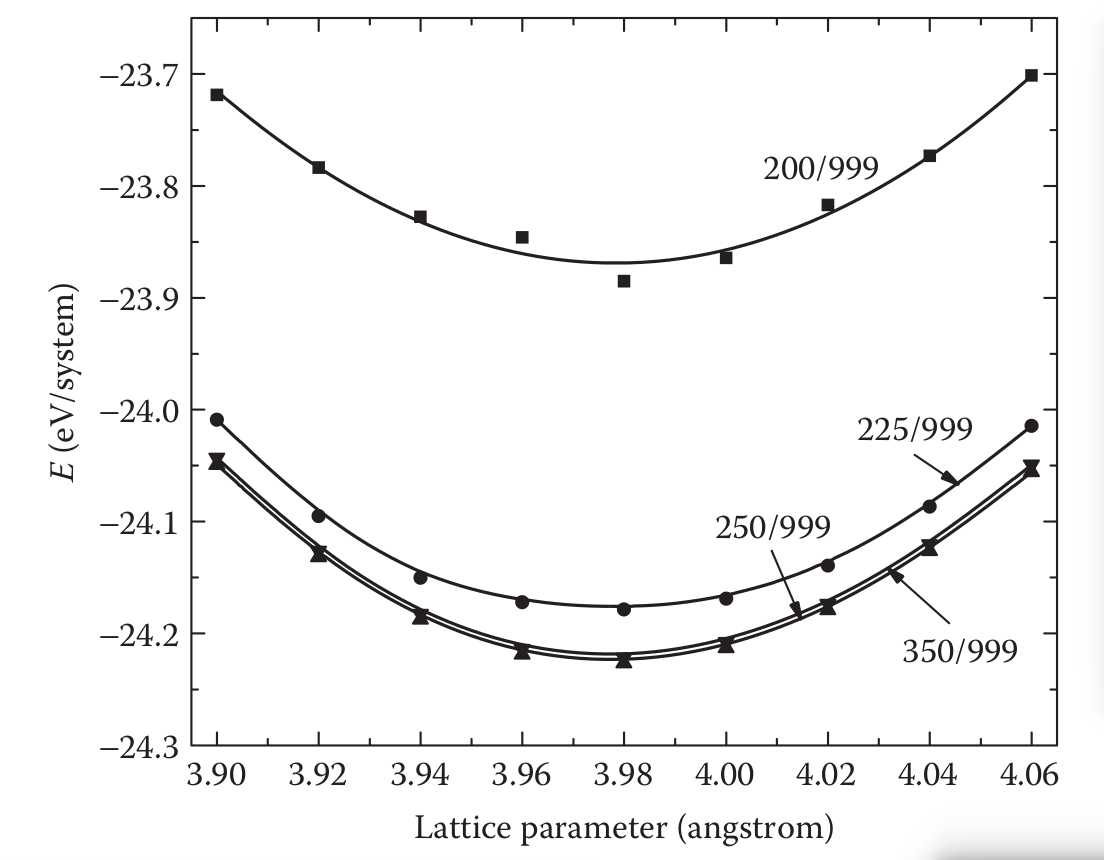
\includegraphics[width=2.8in,viewport=0 11 820 650,clip]{Pt_FCC-Ecut-convergence.png}
\caption{\fontsize{6.2pt}{5.2pt}\selectfont{\textrm{FCC-Pt}截断能收敛测试:~不同截断能下的基态总能曲线($\vec k$-点数目$9\times9\times9$).}}%(与文献\cite{EPJB33-47_2003}图1对比)
\label{Pt_FCC-energy-curve}
\end{figure}
{\fontsize{7.2pt}{5.2pt}\selectfont{不难预见,随着截断能的增加,计算时长将会增加($\vec k$点增加的情形类似)}}
}
%。关于\textit{ENCUT}的设置注意以下事项:
%\begin{itemize}
%	\item 对于多元素组分的体系,一般默认最高的截断能作为体系截断能;
%	\item 对于需要比照的体系,计算时应将\textit{ENCUT}和\textrm{KPOINTS}的数值设置成相同;
%	\item 对于晶格形状和体积都可以弛豫(\textit{ISIF}=3)的体系,一般\textit{ENCUT}比默认值增大$\sim30\%$,并设置参数\textit{PREC}=\textrm{accurate}
%\end{itemize}

%由截断能的定理式\eqref{eq:Ecut}可知,随着\textit{ENCUT}的增大,每个\textrm{k}-点上用于展开轨道的平面波数目的相应变化,将会呈现$\mathrm{N}_{\mathrm{PW}}\propto E_{\mathrm{cut}}^{3/2}$的基本规律。这一点可以在\textrm{OUTCAR}中查找平面波数目得到印证。命令为:~\\
%\textcolor{magenta}{\textrm{grep~\`~plane waves\`~OUTCAR}}\\
%图\ref{Pt_FCC-PW}给出当截断能\textit{ENCUT}=250\textrm{~eV}时,部分$\vec k$点上用于展开波函数的平面波基组的数目。
%\begin{figure}[h!]
%\centering
%\vskip -8pt
%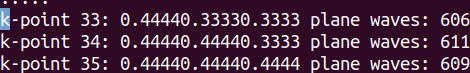
\includegraphics[height=0.6in,viewport=0 0 500 80,clip]{Pt_FCC-PW.png}
%\caption{\small \textrm{FCC-Pt}截断能收敛测试:~截断能为250\textrm{~eV}时各$\vec k$点的平面波基数目(部分).}%(与文献\cite{EPJB33-47_2003}图1对比)
%\label{Pt_FCC-PW}
%\end{figure}
%
%此外,在\textrm{OUTCAR}中,\textit{NPLWV}表示\textrm{FFT}变换的总的网格点数($\mathit{NGX}\times\mathit{NGY}\times\mathit{NGZ}$),这里$\mathit{NGX}$, $\mathit{NGY}$和$\mathit{NGZ}$分别对应$x$-,$y$-和$z$-方向的网格点数。如果对比不同晶体结构的\textrm{Pt}体系,如六方密堆积的\textrm{HCP-Pt}和体心立方的\textrm{BCC-Pt}完成相同的结构弛豫,我们将会发现,面心立方结构\textrm{FCC-Pt}具有最低的基态能量,亦即具有是最稳定的基态结构。这部分内容作为课后练习,留给大家自行完成并验证上述结论。

%\subsection{$\vec k$点收敛测试}
\frame
{
	\frametitle{$\vec k$点收敛测试}
一旦确定合适的\textrm{ENCUT},可用类似的方式确定$\vec k$点数目%。利用晶体对称性,倒空间中的均匀网格点将被约化到不可约\textrm{Brillouin}区(\textrm{Irreducible Brillouin Zone,~IBZ})中。这些不可约$\vec k$-点作为$\vec k$空间的积分权重点,将会用于体系物性计算。当确定参数\textit{ENCUT}为250\textrm{~eV},平衡态晶格常数为$3.977\mathrm{\AA}$后,依次增加$\vec k$-空间网格布点(由$2\times2\times2$到$10\times10\times10$),直至总能的能量差是收敛到$\sim1\mathrm{meV}$。
%
%输出文件\textrm{IBZKPT}中保存的是\textrm{IBZ}区域的$\vec k$点信息,随着$\vec k$点数的增加,\textrm{IBZ}的网格点将由1增大到35。
\begin{figure}[h!]
\centering
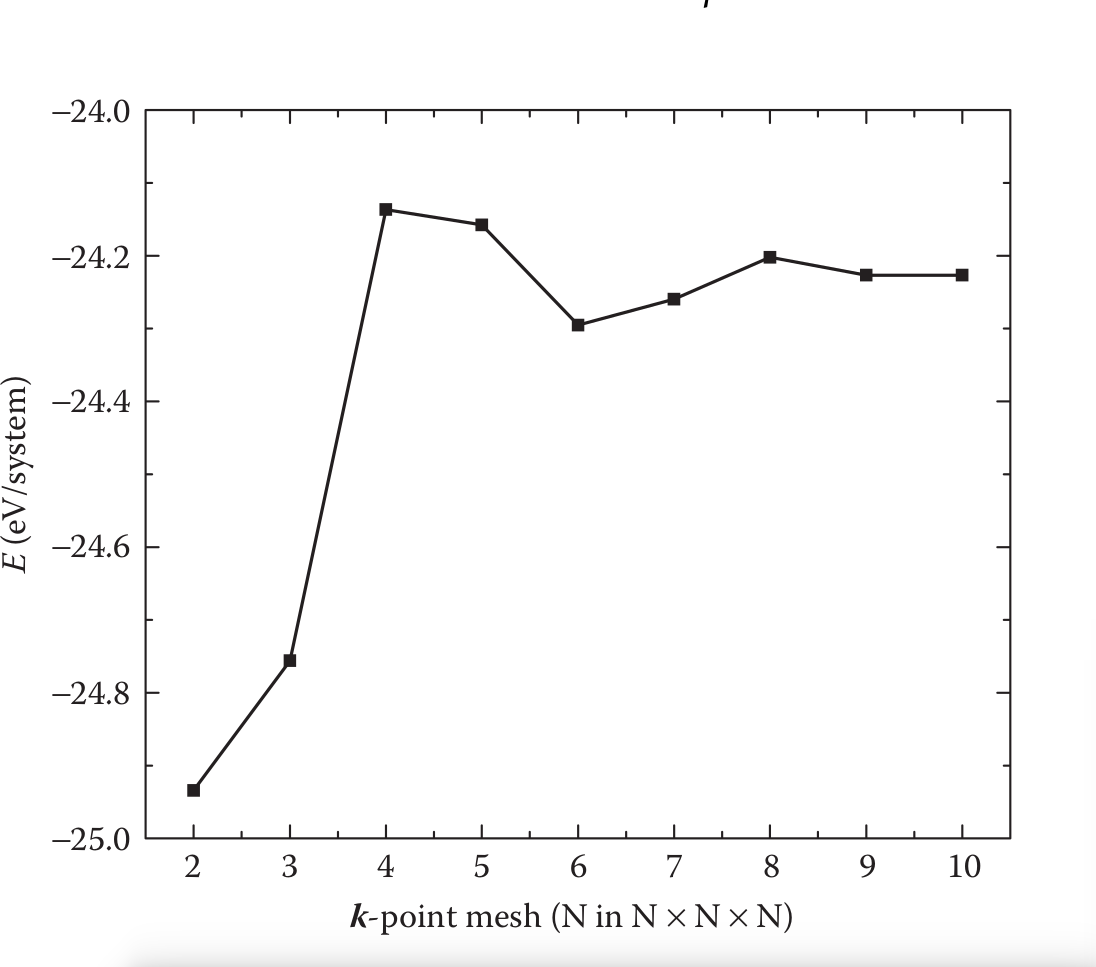
\includegraphics[width=2.8in,viewport=0 11 820 650,clip]{Pt_FCC-kpoint-convergence.png}
\caption{\fontsize{6.2pt}{5.2pt}\selectfont{\textrm{FCC-Pt}截断能收敛测试:~基态总能随$\vec k$-点变化的曲线(截断能\textrm{ENCUT}=250\textrm{~eV}).}}%(与文献\cite{EPJB33-47_2003}图1对比)
\label{Pt_FCC-kpoint-curve}
\end{figure}
{\fontsize{6.2pt}{5.2pt}\selectfont{$\vec k$-点收敛测试与\textit{ENCUT}收敛的情形类似}}%,结果如图\ref{Pt_FCC-kpoint-curve}所示。从图中不难看出,对于当前体系,$9\times9\times9$的网格点能保证足够精度。
%需要指出的是,从文件\textrm{IBZKPT}中的$\vec k$点分布看,采用\textrm{Monkhorst-Pack}布点方案,将每个维度格点剖分成偶数时,$\vec k$空间的网格点分布会更均匀。
}
\section{{\rm Si}的电子结构:~态密度与能带}\label{Sec:Si-band}
\frame
{
	\frametitle{\textrm{Si}的初基原胞:~\textrm{FCC}}
\vspace*{-13pt}
\begin{figure}[h!]
\centering
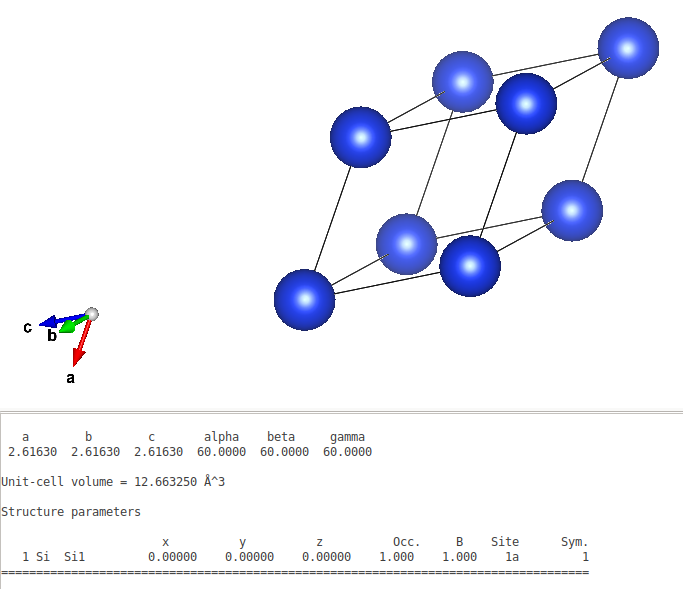
\includegraphics[height=1.78in]{Figures/VASP_example-Si_POSCAR-1-Fig.png}
\vskip 1pt
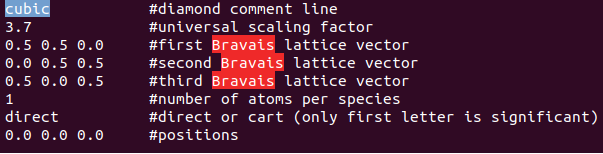
\includegraphics[height=0.98in]{Figures/VASP_example-Si_POSCAR-1.png}
%\caption{\tiny \textrm{The structure of TiC.}}%(与文献\cite{EPJB33-47_2003}图1对比)
\label{Fig:VASP-Si_POSCAR}
\end{figure}
}

\frame
{
	\frametitle{\textrm{Si}的初始计算:~输入文件}
\vspace*{-5pt}
\begin{figure}[h!]
\centering
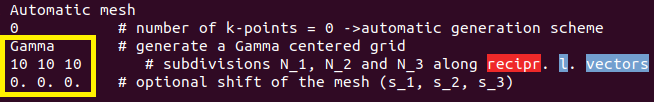
\includegraphics[height=0.62in]{Figures/VASP_example-Si_KPOINTS-G.png}
\vskip 4pt
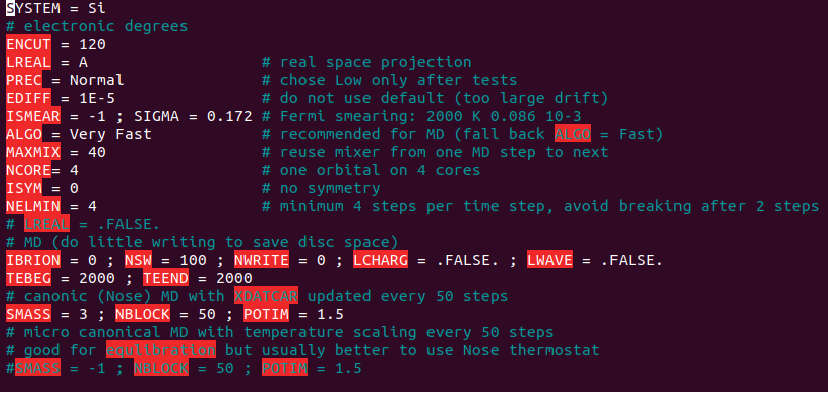
\includegraphics[height=1.88in]{Figures/VASP_example-Si_INCAR-dyn.png}
%\caption{\tiny \textrm{The structure of TiC.}}%(与文献\cite{EPJB33-47_2003}图1对比)
\label{Fig:VASP-Si_KPOINT-INCAR}
\end{figure}
}

%\frame
%{
%	\frametitle{\textrm{Si}的初始计算:~\textrm{POTCAR}}
%\vspace*{-13pt}
%\begin{figure}[h!]
%\centering
%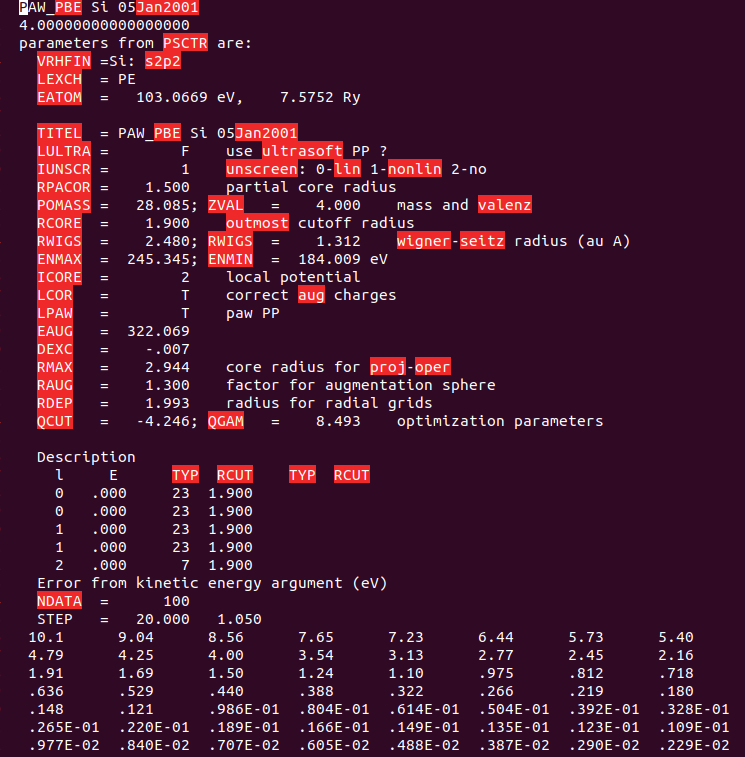
\includegraphics[height=2.88in]{Figures/VASP_example-Si_POTCAR.png}
%%\caption{\tiny \textrm{The structure of TiC.}}%(与文献\cite{EPJB33-47_2003}图1对比)
%\label{Fig:VASP-Si_POTCAR}
%\end{figure}
%}
%
%\frame
%{
%	\frametitle{\textrm{VASP}计算示范:~\textrm{Si}}
%\vspace*{-10pt}
%\begin{figure}[h!]
%\centering
%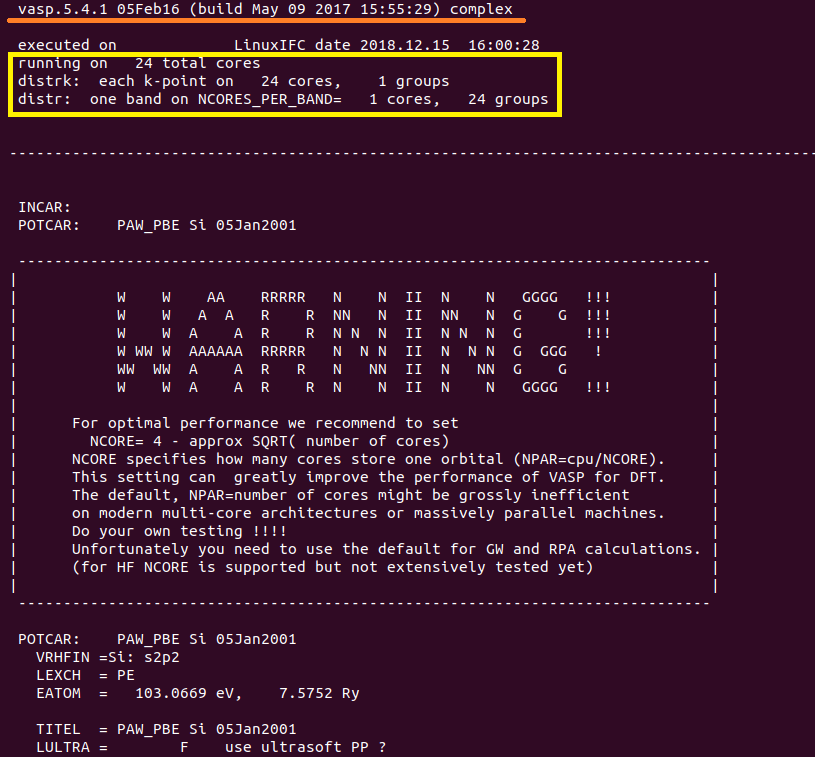
\includegraphics[width=3.0in]{Figures/VASP_example-Si_OUTCAR-1.png}
%%\caption{\tiny \textrm{The structure of TiC.}}%(与文献\cite{EPJB33-47_2003}图1对比)
%\label{Fig:VASP-Si_OUTCAR-part1}
%\end{figure}
%}
%
%\frame
%{
%	\frametitle{\textrm{VASP}计算示范:~\textrm{Si}}
%\vspace*{-10pt}
%\begin{figure}[h!]
%\centering
%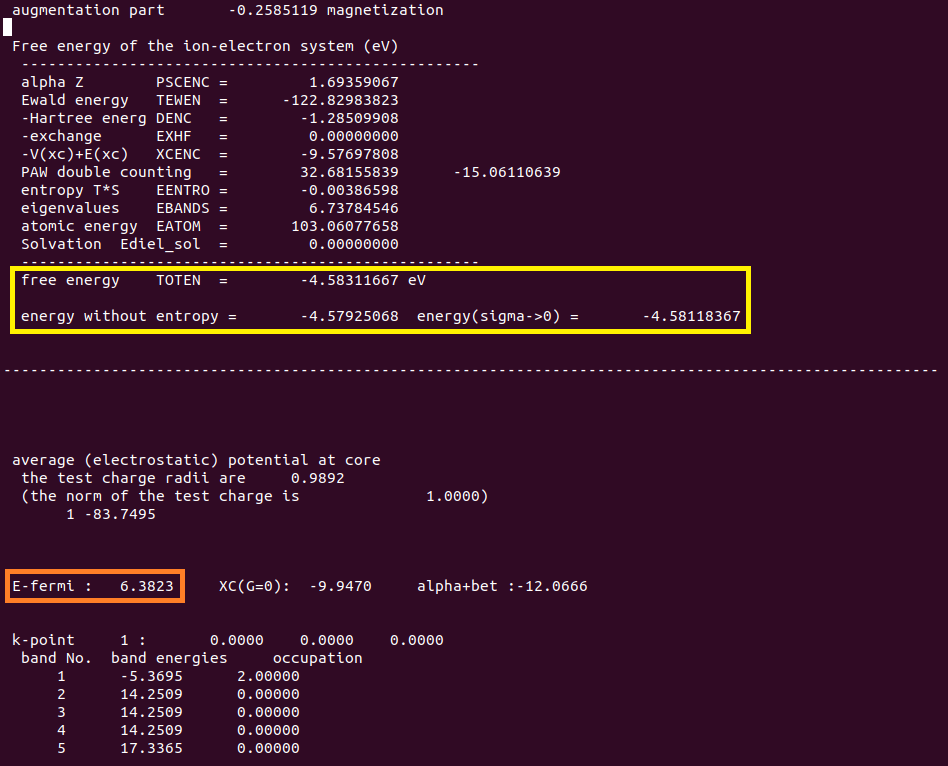
\includegraphics[width=3.5in]{Figures/VASP_example-Si_OUTCAR-2.png}
%%\caption{\tiny \textrm{The structure of TiC.}}%(与文献\cite{EPJB33-47_2003}图1对比)
%\label{Fig:VASP-Si_OUTCAR-part2}
%\end{figure}
%}
%
\frame
{
	\frametitle{\textrm{Si}的静态计算}
%静态计算是获得电子基态信息的重要步骤,在
静态计算:~确定基态电荷密度
\vskip 5pt
{\fontsize{8.5pt}{5.2pt}\selectfont{\textcolor{blue}{材料电子学性质计算的起点}}}
%静态计算时,\textrm{INCAR}中设置参数\textit{ENCUT}=250;~\textrm{KPOINTS}的$\vec k$点数目设为$7\times7\times7$。金刚石结构的\textrm{Si}晶胞可以视为两套\textrm{FCC}结构错开($a$/4,$a$/4,$a$/4)排列,这里$a$即立方晶胞参数。所以\textrm{POSCAR}文件可以写成包含两个\textrm{Si}原子的\textrm{FCC}初基原胞\textrm{(primitive unit cell)}%:如图\ref{Si_POSCAR}所示。
\begin{figure}[h!]
\centering
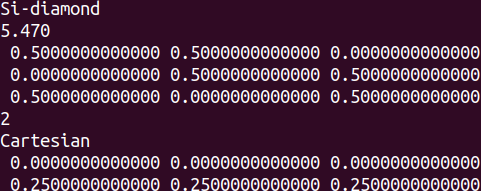
\includegraphics[height=1.2in,viewport=0 0 370 150,clip]{Si_POSCAR.png}
%\includegraphics[height=1.8in,width=4.in,viewport=30 210 570 440,clip]{PAW_projector.eps}
\caption{\fontsize{6.2pt}{5.2pt}\selectfont{\textrm{Si}的初基原胞的\textrm{POSCAR}文件.}}%(与文献\cite{EPJB33-47_2003}图1对比)
\label{Si_POSCAR}
\end{figure}
{\fontsize{7.2pt}{5.2pt}\selectfont{\textrm{Si}晶胞是金刚石结构,晶胞参数$a_0=5.47\mathrm{\AA}$由结构弛豫确定}}%为了得到\textrm{Si}的电子结构,必须要完成两组连续计算:~即通过静态计算得到迭代收敛的基态电子密度,随后用获得的电子密度,按特定的对称性方向,直接计算(无需自洽迭代)得到能带。
%计算需要的\textrm{Si}原子的\textrm{POTCAR}文件可以从\textrm{VASP}的赝势库中知道并保存到当前目录,内容如图\ref{Si_POTCAR}。
%\begin{figure}[h!]
%\centering
%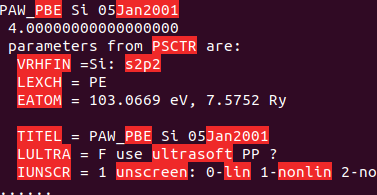
\includegraphics[height=1.2in,viewport=0 0 400 200,clip]{Si_POTCAR.png}
%%\includegraphics[height=1.8in,width=4.in,viewport=30 210 570 440,clip]{PAW_projector.eps}
%\caption{\fontsize{6.2pt}{5.2pt}\selectfont{\textrm{Si}的\textrm{POTCAR}.文件(部分)}}%(与文献\cite{EPJB33-47_2003}图1对比)
%\label{Si_POTCAR}
%\end{figure}
\vskip 6pt
{\fontsize{8.5pt}{5.2pt}\selectfont{静态计算完毕,可以从文件\textrm{OSZICAR}得到体系的基态能量,电荷密度则保存到文件\textrm{CHGCAR}中}}
}

\frame
{
	\frametitle{静态计算:~\textrm{Si}的态密度}
\vspace*{-10pt}
\begin{figure}[h!]
\centering
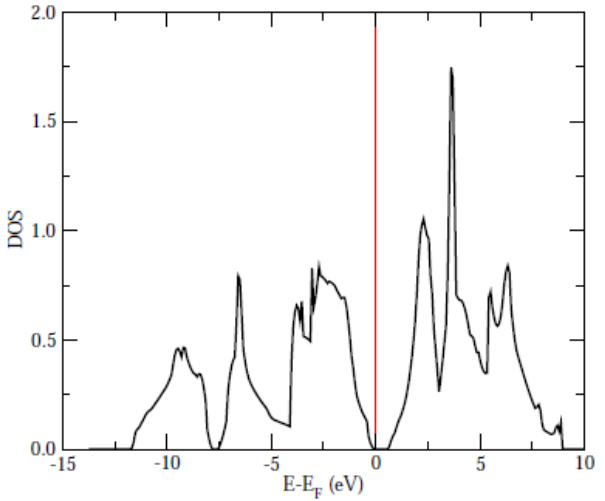
\includegraphics[width=3.5in]{Figures/VASP_cdSi_1.png}
%\caption{\tiny \textrm{The structure of TiC.}}%(与文献\cite{EPJB33-47_2003}图1对比)
\label{Fig:VASP-Si_DOS}
\end{figure}
}

%\subsection{Si的能带结构计算}
\frame
{
	\frametitle{能带计算与$\vec k$点选择}
%一般地,波矢$\vec k $的取值是三维空间(第一\textrm{Brillouin}区)中的矢量。在
	%表\ref{Tabble-kpath}给出的是\textrm{FCC}结构的第一\textrm{Brillouin}区的高对称性$\vec k$点列表。
\begin{minipage}{1.0\textwidth}
\begin{table}[!h]
\tabcolsep 0pt \vspace*{-12pt}
\fontsize{7.2pt}{5.2pt}\selectfont{
%\begin{center}
\centering
\caption{\fontsize{6.2pt}{5.2pt}\selectfont{\textrm{FCC}的第一\textrm{Brillouin}区中高对称性点的列表}}\label{Table-kpath}
\def\temptablewidth{0.95\textwidth}
\renewcommand\arraystretch{0.8} %表格宽度控制(普通表格宽度的两倍)
\rule{\temptablewidth}{1pt}
\begin{tabular*} {\temptablewidth}{@{\extracolsep{\fill}}c@{\extracolsep{\fill}}c@{\extracolsep{\fill}}c}
%-------------------------------------------------------------------------------------------------------------------------
	&\textrm{Reciprocal coordinates} &\textrm{Cartesian coordinates}\\
	\textrm{Points}	&\textrm{(unit of $b_1,b_2,b_3$)} &\textrm{unit of $2\pi/a$} \\\hline
	$\Gamma$ &0~~0~~0 &0~~0~~0 \\
	X &1/2~~0~~1/2 &0~~1~~0 \\
	W &3/4~~1/2~~1/4 &0~~1/2~~1 \\
	L &1/2~~1/2~~1/2 &1/2~~1/2~~1/2 \\
	$\Delta$ &1/4~~0~~1/4 &0~~1/2~~0 \\
	$\Lambda$ &1/ 4~~1/4~~1/4 &1/4~~1/4~~1/4 \\
\end{tabular*}
\rule{\temptablewidth}{1pt}
}
%\end{center}
\end{table}
\end{minipage}
\begin{figure}[h!]
	\vskip -8pt
\centering 
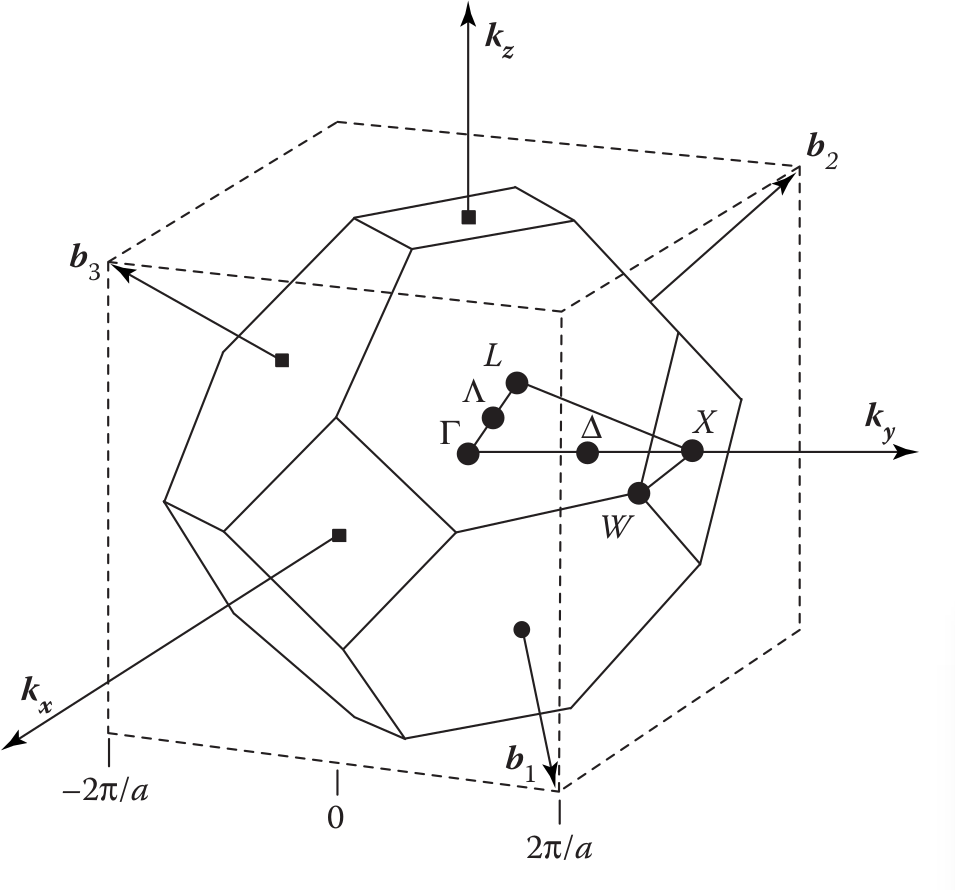
\includegraphics[height=1.7in,viewport=0 0 680 680,clip]{VASP_train-FCC-BZ.png}
%\includegraphics[height=1.8in,width=4.in,viewport=30 210 570 440,clip]{PAW_projector.eps}
\caption{\fontsize{6.2pt}{5.2pt}\selectfont{\textrm{Brillouin}区为\textrm{FCC}时的空间结构和$\vec k$-点路径关系.}}%(与文献\cite{EPJB33-47_2003}图1对比)
\label{VASP_train-FCC-BZ}
\end{figure}
	{\fontsize{7.5pt}{5.2pt}\selectfont{能带表示中的波矢$\vec k$选择:~沿不可约第一\textrm{Brillouin}区的高对称性点连线}}
%因此,为了绘制平滑的能带曲线,需要在\textrm{KPOINTS}文件中指定足够多的$\vec k$点,能带计算时,只需针对这些指定的$\vec k$点计算各轨道的能量本征值。%如图\ref{Si_KPOINTS}所示:
}

\frame
{
	\frametitle{\textrm{Si}能带计算}

%为了完成能带计算,主要是\textrm{CHGCAR}文件,其余文件改动极少。
%\subsubsection{\rm{INCAR}}%如图\ref{Si_Band-INCAR}所示。这里
%\subsubsection{\rm{KPOINTS}}
{\fontsize{7.5pt}{5.2pt}\selectfont{由\textrm{Brillouin}区$\vec k$点连线,确定\textrm{KPOINTS}文件的$\vec k$点分布:}}\\%如图所示\ref{VASP_train-FCC-BZ}。
{\fontsize{6.2pt}{5.2pt}\selectfont{沿$\vec k$点路线$\mathrm{W}-\mathrm{L}-\Gamma-\mathrm{X}-\mathrm{W}$共计80个$\vec k$点(20点/连线$\times$4组连线)}%的\textrm{KPOINTS}文件%,对应
\begin{figure}[h!]
	\vskip -5pt
\centering 
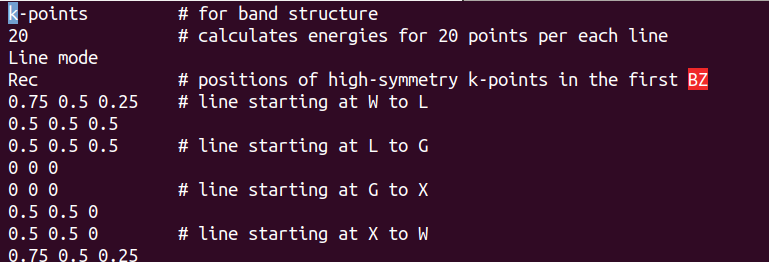
\includegraphics[width=3.6in,viewport=0 0 540 210,clip]{Si_KPOINTS.png}
%\includegraphics[height=1.8in,width=4.in,viewport=30 210 570 440,clip]{PAW_projector.eps}
\caption{\fontsize{6.2pt}{5.2pt}\selectfont{\textrm{Si}的能带计算时\textrm{KPOINTS}的设置.}}%(与文献\cite{EPJB33-47_2003}图1对比)
\label{Si_KPOINTS}
\end{figure}
%图\ref{Si_KPOINTS}给出的是\textrm{VASP}计算
}
\begin{figure}[h!] 
	\vskip -5pt
\centering
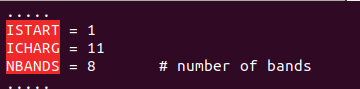
\includegraphics[height=0.5in,viewport=0 0 330 80,clip]{Si_Band-INCAR.png}
%\includegraphics[height=1.8in,width=4.in,viewport=30 210 570 440,clip]{PAW_projector.eps}
\caption{\fontsize{6.2pt}{5.2pt}\selectfont{\textrm{Si}的能带计算中的\textrm{INCAR}设置.}}%(与文献\cite{EPJB33-47_2003}图1对比)
\label{Si_Band-INCAR}
\end{figure}
{\fontsize{7.5pt}{5.2pt}\selectfont{静态计算完毕,根据能带计算需要,修改\textrm{INCAR}文件参数:~设置\textcolor{cyan}{\textit{ICHARG}}=11,电荷密度来自静态计算\textrm{CHGCAR},在计算中保持不变}}
}

\frame
{
	\frametitle{\textrm{Si}能带}
%图\ref{Si_Band-DOS}给出绘制的能带图,可见按照当前的$\vec k$点路径选择,。
\begin{figure}[h!]
	\vskip -8pt
\centering
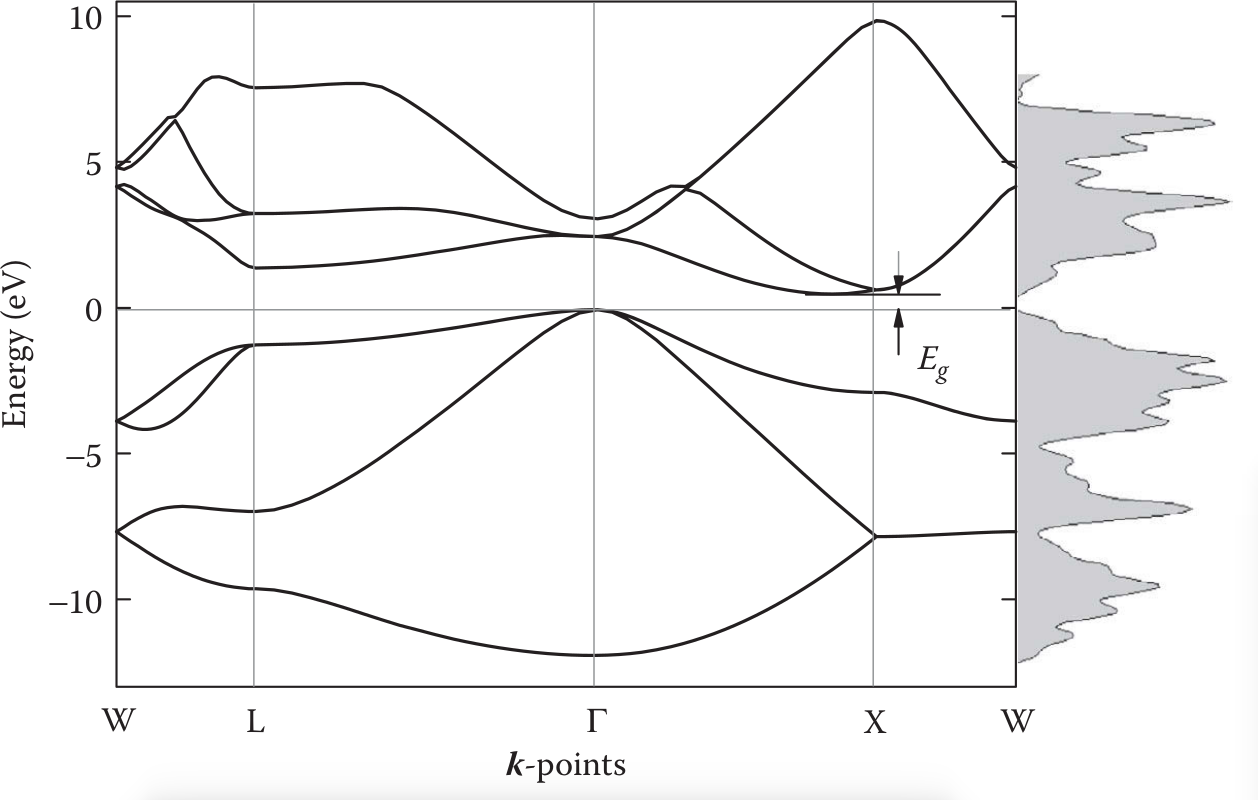
\includegraphics[width=3.5in,viewport=0 10 920 610,clip]{Si_Band-DOS.png}
%\includegraphics[height=1.8in,width=4.in,viewport=30 210 570 440,clip]{PAW_projector.eps}
\caption{\fontsize{6.2pt}{5.2pt}\selectfont{\textrm{Si}的能带和相应的态密度图,从能带图看出\textrm{Si}是间接带隙半导体.}}%(与文献\cite{EPJB33-47_2003}图1对比)
\label{Si_Band-DOS}
\end{figure}
{\fontsize{6.2pt}{5.2pt}\selectfont{\textrm{Si}是%间接带隙
半导体,带隙$E_g=0.61\textrm{eV}$%是$\Gamma$点和$X$点之间的带隙值,同时也是图中所有$\vec k$点之间最小的能量差。
~(该值仅为实验测得带隙的$1/2$,因\textrm{DFT}先天不足,低估带隙)}}
%不过除了对带隙的低估,\textrm{DFT}计算的色散关系(能量在倒空间分布关系)是完全正确的,比如\textrm{Fermi}面附近有四个价带,四个导带,能量$\varepsilon_{\vec k}^n$随$\vec k$空间的变化逐渐改变,因此\textrm{DFT}理论的计算定性是完全正确的。实际上,其他物理量(比如波函数和电子密度),也和能量本征值有类似的倒空间分布关系。表明这样的$\vec k$点采样是合理的,能够表现物理量在不可约\textrm{Brillouin}区的定量变化。
}

%\frame
%{
%	\frametitle{\textrm{Si}的能带}
%%\vspace*{5pt}
%\begin{figure}[h!]
%\centering
%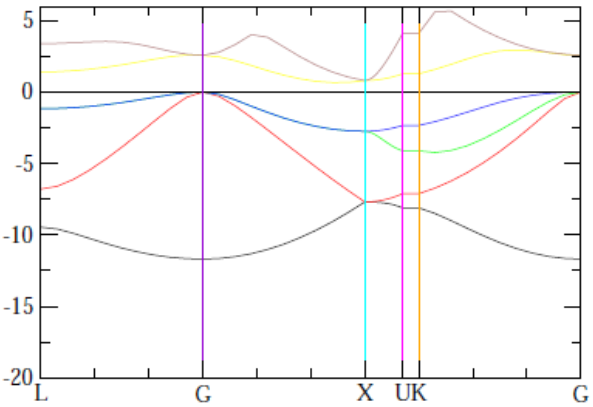
\includegraphics[width=4.0in]{Figures/VASP_cdSi_2.png}
%%\caption{\tiny \textrm{The structure of TiC.}}%(与文献\cite{EPJB33-47_2003}图1对比)
%\label{Fig:VASP-Si_Band}
%\end{figure}
%}
%
\frame
{
	\frametitle{\textrm{Si}的能带可视化:~\textrm{p4vasp}}
%\vspace*{5pt}
\begin{figure}[h!]
\centering
\includegraphics[width=4.0in]{Figures/VASP_cdSi_3.png}
%\caption{\tiny \textrm{The structure of TiC.}}%(与文献\cite{EPJB33-47_2003}图1对比)
\label{Fig:VASP-Si_p4vasp}
\end{figure}
}

%\subsubsection{\rm{能带中的本征值}}
\frame
{
	\frametitle{\textrm{Si}能带与本征值}
%因为能带计算是非自洽迭代计算,计算出来能量本征值$\varepsilon_{\vec k}^n$写入\textrm{EIGENVAL}文件中,用于绘制能带图。如图\ref{Si_Band-EIGENVAL}所示
	{\fontsize{7.2pt}{5.2pt}\selectfont{由\textrm{OUTCAR}可知\textrm{Fermi}能级为5.6980\textrm{eV}}}%)设为0~\textrm{eV},可以得到$\vec k$点和能量本征值关系的数据文件\textrm{Si-band.dat},内容如图\ref{Si_Band-data}所示
\begin{figure}[h!]
	\vskip -3pt
\centering
\includegraphics[width=4.0in,viewport=0 0 640 375,clip]{Si_Band-EIGENVAL.png}
%\includegraphics[height=1.8in,width=4.in,viewport=30 210 570 440,clip]{PAW_projector.eps}
\caption{\fontsize{6.2pt}{5.2pt}\selectfont{\textrm{VASP}计算\textrm{Si}的能量本征值文件\textrm{EIGENVAL}(部分).}}%(与文献\cite{EPJB33-47_2003}图1对比)
\label{Si_Band-EIGENVAL}
\end{figure}
%文件\textrm{EIGENVAL}中第一行是倒晶格中的$\vec k$点位置,随后8行是对应的8个能带的能量本征值:~其中前4个(\textrm{No.}~1-4)能级表示价带,是0\textrm{K}下的占据态。从\textrm{EIGENVAL}文件中提取出各$\vec k$点的能量本征值$\varepsilon_{\vec k}^n$,并将\textrm{Fermi}能级设置为0~(可以用本讲义提供的脚本\textcolor{blue}{\textrm{vasp\_to\_image.py}}实现)。运行该脚本,将\textrm{Fermi}能级(

%\begin{figure}[h!]
%\centering
%\includegraphics[height=1.2in,viewport=0 0 540 140,clip]{Si_Band-data.png}
%%\includegraphics[height=1.8in,width=4.in,viewport=30 210 570 440,clip]{PAW_projector.eps}
%\caption{\small \textrm{用于绘制\textrm{Si}能带结构的数据.}}%(与文献\cite{EPJB33-47_2003}图1对比)
%\label{Si_Band-data}
%\end{figure}
}

\section{{\rm Pt}超晶胞计算}\label{Sec:bulk-Pt}
%下面我们将学习由32个\textrm{Pt}原子构成的超晶胞(\textrm{FCC}晶胞按$2\times2\times2$堆积得到)的基本的物理性质计算:~重点掌握内聚能\textrm{(cohesive energy)}和空位形成能\textrm{(vavanvy formation energy)}的计算。为简明起见,前面介绍过的参数,今后不再作详细说明。
%\subsection{Pt超晶胞的内聚能计算}
\frame
{
	\frametitle{\textrm{Pt}超晶胞内聚能计算:~输入文件}
%为了计算内聚能,首先计算理想超晶胞的\textrm{Pt}基态能量。输入控制文件\textrm{INCAR}的修改部分如图\ref{Pt_Bulk-INCAR-modified}所示:~
	{\fontsize{7.4pt}{5.2pt}\selectfont{计算中不再要求输出电荷密度和波函数到\textrm{CHGCAR}和\textrm{WAVECAR},设置控制参数\textcolor{blue}{\textit{ISYM}}=1}}
\begin{figure}[h!]
\centering
\includegraphics[height=0.8in,viewport=0 20 340 118,clip]{Pt_Bulk-INCAR.png}
%\includegraphics[height=1.8in,width=4.in,viewport=30 210 570 440,clip]{PAW_projector.eps}
\caption{\fontsize{6.2pt}{5.2pt}\selectfont{\textrm{计算\textrm{Pt}超晶胞时\textrm{INCAR}文件的修改部分.}}}%(与文献\cite{EPJB33-47_2003}图1对比)
\label{Pt_Bulk-INCAR-modified}
\end{figure}
\begin{figure}[h!]
\centering
\vskip -3pt
\includegraphics[height=0.8in,viewport=0 20 240 108,clip]{Pt_Bulk-KPOINTS.png}
%\includegraphics[height=1.8in,width=4.in,viewport=30 210 570 440,clip]{PAW_projector.eps}
\caption{\fontsize{6.2pt}{5.2pt}\selectfont{\textrm{计算\textrm{Pt}超晶胞时的\textrm{KPOINTS}文件.}}}%(与文献\cite{EPJB33-47_2003}图1对比)
\label{Pt_Bulk-KPOINTS}
\end{figure}
{\fontsize{6.2pt}{5.2pt}\selectfont{超晶胞是由8倍的\textrm{FCC-Pt}构成,$\vec k$-点数约简为$5\times5\times5$}}%,\textrm{KPOINTS}文件如图\ref{Pt_Bulk-KPOINTS}所示:~
}

\frame
{
	\frametitle{\textrm{Pt}超晶胞内聚能计算:~输入文件}
%考虑到\ref{Sec:FCC-Pt}已经得到\textrm{FCC-Pt}结构弛豫后的晶胞,因此$2\times2\times2$堆积的超晶胞中原子起始结构如图\ref{Pt_Bulk-POSCAR}所示。虽然\textrm{INCAR}中的控制参数允许晶胞结构弛豫,超晶胞的\textrm{POSCAR}文件中的原子也仍保持可移动状态,但可以预见,体系的弛豫计算不应该带来很显著的形变。
\begin{figure}[h!]
\centering
\vskip -5pt
\includegraphics[height=2.0in,viewport=0 25 500 270,clip]{Pt_Bulk-POSCAR.png}
%\includegraphics[height=1.8in,width=4.in,viewport=30 210 570 440,clip]{PAW_projector.eps}
\caption{\fontsize{6.2pt}{5.2pt}\selectfont{\textrm{计算\textrm{Pt}超晶胞时的\textrm{POSCAR}文件(部分).}}}%(与文献\cite{EPJB33-47_2003}图1对比)
\label{Pt_Bulk-POSCAR}
\end{figure}
}

\frame
{
	\frametitle{\textrm{Pt}超晶胞内聚能计算:~运算输出}
%用\ref{Sec:FCC-Pt}的\textrm{shell}脚本\textcolor{green}{\textrm{run.vasp}}提交计算任务至后台运行,计算过程中可以检查输出文件\textrm{nohup.out}或\textrm{OSZICAR}的内容可以监控计算过程,图\ref{Pt_Bulk-OSZICAR}给出\textrm{nohup.out}的部分结果:
\begin{figure}[h!]
\centering
\hspace*{-5pt}
\includegraphics[width=4.0in,viewport=0 0 950 215,clip]{Pt_Bulk-OSZICAR.png}
%\includegraphics[height=1.8in,width=4.in,viewport=30 210 570 440,clip]{PAW_projector.eps}
\caption{\fontsize{6.2pt}{5.2pt}\selectfont{\textrm{计算\textrm{Pt}超晶胞时的迭代输出\textrm{OSZICAR}文件(局部).}}}%(与文献\cite{EPJB33-47_2003}图1对比)
\label{Pt_Bulk-OSZICAR}
\end{figure}
{\fontsize{7.2pt}{5.2pt}\selectfont{\textrm{VASP}程序为快速收敛,设定完成前五次电子步迭代后,才开始电荷密度的迭代,所以最初\textrm{5}次电子步迭代时,没有\textrm{rms(c)}输出%。电子步结束时,最后一行的\textrm{F}表示电子步达到收敛的自由能,

根据同一行的$\mathrm{E}_0$值(0\textrm{K}时$\sigma\rightarrow0$),可以算出超晶胞中的单个原子\textrm{Pt}的能量为$-193.8569/32=-6.058\mathrm{~eV/atom}$

不难看出,该值比晶格参数为$3.975\mathrm{\AA}$时计算的\textrm{FCC-Pt}的原子能量$-6.056\mathrm{eV/atom}$仅有微小变化}}
}
%如果迭代计算过程中出错,\textrm{VASP}将会输出错误或警告提示信息,并终止程序运行。此外也可以通过\textrm{kill}命令终止程序。命令为:~\\
%\textcolor{magenta}{\textrm{killall -9 VASP\_pid}}\\
%这里\textrm{VASP\_pid}是当前执行的\textrm{VASP}进程号。
%
%如果计算过程中发现有参数或设置问题,可以在计算目录中产生一个\textrm{STOPCAR}文件,并向其中增添一行内容:~\\
%\textit{LSTOP}=\textrm{.TRUE.}\\
%则正在运行的\textrm{VASP}程序会在当前离子步结束并输出\textrm{WAVECAR}和\textrm{CHGCAR}后,进入下一离子步计算时退出运行。一般用户可以在修正发现的错误后,在现有计算基础上,继续向下完成整个计算任务。

%\subsubsection{内聚能}
\frame
{
	\frametitle{内聚能计算}
内聚能\textrm{(Cohesive energy) $E_{\mathrm{coh}}$}:~\\
体相的平均原子能量和自由原子能量$E_{\mathrm{atom}}$的能量差
\vskip 3pt
{\fontsize{7.5pt}{5.2pt}\selectfont{内聚能是衡量原子构成固体时原子间相互作用强弱的参数}}%,也是材料的一个基本属性。换句话说,
\vskip 5pt
内聚能可通过固体原子在平衡态附近的极小值扣除自由原子能量得到:%。因此可以用以下两个值计算内聚能:~
\begin{displaymath}
	\begin{aligned}
		E_{\mathrm{bulk}}&=-193.85695/32=-6.058~\mathrm{eV/atom}\\
		E_{\mathrm{coh}}&=E_{\mathrm{atom}}-E_{\mathrm{bulk}}=(-0.528)-(-6.058)=5.53\mathrm{eV/atom}
	\end{aligned}
\end{displaymath}
{\fontsize{7.5pt}{5.2pt}\selectfont{该值与文献记载的计算值5.53\textrm{~eV/atom}\upcite{PRB78-205302_2008}一致,与实验值5.45\textrm{~eV/atom}\upcite{Landolt-Bornstein}的数值吻合}}
}

%\subsection{\rm{Pt}的空位生成能计算}
\frame
{
	\frametitle{\textrm{Pt}的空位生成能计算:~模型设计}
室温条件下,金属体相内空位浓度约为$10^{-6}$量级
\vskip 5pt
{\fontsize{7.5pt}{5.2pt}\selectfont{显然不可能为了模拟一个空位,就用$10^6$量级的超晶胞。合理的做法应该是选择合适尺度的超晶胞并设计原子空位,要求超晶胞间空位相互作用可以忽略,由此计算晶格中的空位能}}%。因为计算的超晶胞中仅有一个空位,计算时将\textrm{INCAR}中关闭对称性。

\textrm{POSCAR}文件%可以从之前的超晶胞算例中\textrm{copy}来,
将总的原子扣除位于(0.5,~0.5,~0.5)处的\textrm{Pt}原子,产生空位%,如图\ref{Pt_vacancy-POSCAR}所示:~
\begin{figure}[h!]
\centering
\vskip -3pt
\includegraphics[height=0.85in,viewport=0 15 750 120,clip]{Pt_vacancy-POSCAR.png}
%\includegraphics[height=1.8in,width=4.in,viewport=30 210 570 440,clip]{PAW_projector.eps}
\caption{\fontsize{6.2pt}{5.2pt}\selectfont{\textrm{模拟\textrm{FCC-Pt}超晶胞中含有一个空位时\textrm{POSCAR}文件的修改部分.}}}%(与文献\cite{EPJB33-47_2003}图1对比)
\label{Pt_vacancy-POSCAR}
\end{figure}
}

\frame
{
	\frametitle{\textrm{Pt}的空位生成能计算}
\begin{figure}[h!]
\centering
\includegraphics[height=0.9in,viewport=0 15 370 180,clip]{Pt_vacancy-INCAR.png}
%\includegraphics[height=1.8in,width=4.in,viewport=30 210 570 440,clip]{PAW_projector.eps}
\caption{\fontsize{6.2pt}{5.2pt}\selectfont{\textrm{\textrm{FCC-Pt}超晶胞计算的\textrm{INCAR}文件修改部分.}}}%(与文献\cite{EPJB33-47_2003}图1对比)
\label{Pt_Bulk-INCAR-modified}
\end{figure}
与\textrm{Pt}超晶胞计算类似,由\textrm{OSZICAR}文件可知,含有31个\textrm{Pt}原子和一个空位的超晶胞基态能量是$-186.95325\mathrm{~eV/atom}$
}
%\subsubsection{空位形成能}

\frame
{
	\frametitle{\textrm{Pt}的空位生成能计算}
根据空位形成能$E_{\mathrm{v}}^f$的定义可以有:~
\begin{displaymath}
	\begin{aligned}
		E_{\mathrm{v}}^f=&E_{\mathrm{v}}-\dfrac{N-1}N\times E_{\mathrm{bulk}}\\
		=&-186.95325-\dfrac{31}{32}(-193.85695)\\
		=&0.846\mathrm{eV/atom}
	\end{aligned}
\end{displaymath}
{\fontsize{6.2pt}{5.2pt}\selectfont{$E_{\mathrm{v}}$是含有一个空位的超晶胞基态总能,$N$是理想超晶胞的原子个数,$E_{\mathrm{bulk}}$是理想晶体的总能(算例中值是~$-193.85695~\mathrm{eV}$)}}
%我们这里的

计算结果与其他计算值$0.68\mathrm{~eV/vacancy}$或通过正电子子湮灭测量的值$1.35\mathrm{~eV/vacancy}$\upcite{PSSA102-47_1987}有不小的差别\footnote{\fontsize{6.2pt}{5.2pt}\selectfont{\textrm{Mattsson}等发现,只要引入体系的表面误差校正,就能改善\textrm{Pt}的空位形成能,结果为1.18\textrm{eV/vacancy}\upcite{PRB66-214110_2002}。对于其他的材料,比如\textrm{W}\upcite{JNM383-244_2009}或\ch{SiC}\upcite{JMS44-1828_2009},用\textrm{DFT}计算的缺陷形成能与实验值吻合得比较好}}

由\textrm{CONTCAR}文件中可以看到空位附近原子的弛豫情况%。\textrm{WAVECAR}是二进制文件,保存的是最终得到的电子轨道波函数,亦即\textrm{Kohn-Sham}方程的解。在本次算例中,因为\textrm{INCAR}中的设置,则未将波函数写到\textrm{WAVECAR}中。
}
%\subsubsection{\rm{CHGCAR}绘图}
\frame
{
	\frametitle{\textrm{CHGCAR}图示}
\textrm{VASP}将电荷密度写到\textrm{CHG}和\textrm{CHGCAR}文件,这两个文件的内容基本相同%,主要包括:~晶格矢量、原子位置,电荷密度等。表示电荷密度的网格与超晶胞的形态成正比,网格的数目由\textrm{OUTCAR}中\textrm{FFT}变换的网格数\textit{NFXF}、\textit{NGYF}和\textit{NGZF}确定。将\textrm{CHGCAR}或\textrm{CHG}中的电荷密度按超晶胞体积划分,就可以得到电荷密度的轮廓。例如,本次练习得到的\textrm{CHGCAR}文件的内容如图\ref{Pt_vacancy-CHGCAR}所示:~
\begin{figure}[h!]
\centering
\vskip -5pt
\includegraphics[width=4.0in,viewport=0 20 490 240,clip]{Pt_vacancy-CONTCAR.png}
%\includegraphics[height=1.8in,width=4.in,viewport=30 210 570 440,clip]{PAW_projector.eps}
\caption{\fontsize{6.2pt}{5.2pt}\selectfont{\textrm{计算\textrm{FCC-Pt}超晶胞出现空位时的\textrm{CHGCAR}文件(部分).}}}%(与文献\cite{EPJB33-47_2003}图1对比)
\label{Pt_vacancy-CHGCAR}
\end{figure}
}

\frame
{
	\frametitle{\textrm{CHGCAR}图示}
	用开源软件如\textcolor{cyan}{\textrm{VASPview}}\footnote{\textrm{VASPview~\url{http://vaspview.sourceforge.net}}}或\textcolor{cyan}{\textrm{VESTA}}\footnote{\textrm{VESTA(ver.2.90.1b),~2011.~\url{http://www.geocities.jp/kmo\_mma/index-en.html}}}可将\textrm{CHGCAR}文件的电荷密度可视化%,效果如图\ref{Pt_vacancy-Density}所示:
\begin{figure}[h!]
\centering
\includegraphics[height=2.0in,viewport=0 0 640 660,clip]{Pt_vacancy-CHGCAR.png}
%\includegraphics[height=1.8in,width=4.in,viewport=30 210 570 440,clip]{PAW_projector.eps}
\caption{\fontsize{6.2pt}{5.2pt}\selectfont{\textrm{计算\textrm{FCC-Pt}超晶胞出现空位时的图像.}}}%(与文献\cite{EPJB33-47_2003}图1对比)
\label{Pt_vacancy-Density}
\end{figure}

注意:~图中空位附近的空白区域(图中只显示了超晶胞的下半区域)和每个原子附近近乎均匀分布的电子分布
}

\frame
{
	\frametitle{其它超晶胞-缺陷性质计算}

类似地,间隙形成能\textrm{(the formation energies of an interstitial)}$E_{\mathrm{inter}}^f$定义为
\begin{displaymath}
	E_{\mathrm{inter}}^f=E_{\mathrm{inter}}^{\mathrm{bulk}}-E^{\mathrm{bulk}}-nE^{\mathrm{atom}}
\end{displaymath}
{\fontsize{6.2pt}{5.2pt}\selectfont{这里$E_{\mathrm{inter}}^{\mathrm{bulk}}$和$E^{\mathrm{bulk}}$是带有间隙的超晶胞和理想超晶胞的总能,$n$是间隙处的原子数目,$E^{\mathrm{atom}}$是孤立原子的能量}}

进一步推广,如果存在两个固相\textrm{A}和{B},它们可以形成\textrm{AB}相,则三个体相的能量能量差
\begin{displaymath}
	\Delta H_{\mathrm{AB}}=E_{\mathrm{AB}}^{\mathrm{bulk}}-E_{\mathrm{A}}^{\mathrm{bulk}}-E_{\mathrm{B}}^{\mathrm{bulk}}
\end{displaymath}
定义为固体生成焓\textrm{(the formation enthalpy)}
\vskip 5pt
\textcolor{purple}{各种缺陷的形成能都可用简化模型来模拟}\\
{\fontsize{7.0pt}{5.2pt}\selectfont{用户在构造包含缺陷的超晶胞时,必须切记,超晶胞要设计得足够大,确保缺陷间的相互作用足够小}}
}

\section{\rm{Pt~(111)}表面的计算}\label{Sec:Surface-Pt}
\frame
{
	\frametitle{材料表面属性}
体相材料的表面有很多基本性质,如
\begin{itemize}
	\item 表面能\textrm{(surface energy)}
	\item 功函数\textrm{(work function)}
	\item 吸附能\textrm{(adsorption energy)}
	\item 吸附原子迁移势垒\textrm{(barrier energy for transport of the adatom)}
\end{itemize}
实际应用中,材料的表面性质具有特殊的重要性%可用来确定材料的用途
{\fontsize{8.0pt}{5.2pt}\selectfont{
	\begin{itemize}
		\item 表面能是表面形貌学研究(向外/向内弛豫、重构、屈服分析)和裂纹扩散到断裂研究的重要因素
		\item 功函数、吸附能/解吸能和势垒能量是研究表面氧化、薄膜表面和纳米结构的生长和稳定、腐蚀、钝化和催化反应的决定因素%。只有真正理解了这些表面现象,才有望从设计层面获得更高性能的材料。本节中,我们将学习构建\textrm{Pt}原子构成的表面,并研究上述提到的表面属性的计算。
	\end{itemize}
}}
}
%\subsection{\rm{Pt~(111)}表面}
\frame
{
	\frametitle{\textrm{Pt~(111)}面\textrm{Slab}:~输入文件}
	{\fontsize{9.5pt}{5.2pt}\selectfont{构建\textrm{Pt~(111)}面\textrm{slab}并计算其基态总能、弛豫能和表面能的计算方案}}%\footnote{\fontsize{6.2pt}{5.2pt}\selectfont{至于选择\textrm{Pt~(111)}面作为研究对象,是因为这个表面在\textrm{Pt}催化材料中研究得最多}}%。这些数据将成为后续进一步计算吸附能和迁移势垒能量的参考基准。
%\subsubsection{\rm{INCAR}}
%\textrm{INCAR}文件的内容如图\ref{Pt_Slab-INCAR}所示:~
\begin{figure}[h!]
\centering
\vskip -5pt
\includegraphics[height=1.5in,viewport=0 10 690 388,clip]{Pt_Slab-INCAR.png}
%\includegraphics[height=1.8in,width=4.in,viewport=30 210 570 440,clip]{PAW_projector.eps}
\caption{\fontsize{6.2pt}{5.2pt}\selectfont{\textrm{计算\textrm{Pt}表面时\textrm{INCAR}文件.}}}%(与文献\cite{EPJB33-47_2003}图1对比)
\label{Pt_Slab-INCAR}
\end{figure}
%\subsubsection{\rm{KPOINTS}}
%\textrm{KPOINTS}内容如图\ref{Pt_Slab-KPOINTS}所示:~
\begin{figure}[h!]
\centering
\vskip -5pt
\includegraphics[height=0.4in,viewport=0 10 400 98,clip]{Pt_Slab-KPOINTS.png}
%\includegraphics[height=1.8in,width=4.in,viewport=30 210 570 440,clip]{PAW_projector.eps}
\caption{\fontsize{6.2pt}{5.2pt}\selectfont{\textrm{计算\textrm{Pt}表面时\textrm{KPOINTS}文件.}}}%(与文献\cite{EPJB33-47_2003}图1对比)
\label{Pt_Slab-KPOINTS}
\end{figure}
}
%\subsubsection{\rm{POSCAR}}
\frame
{
	\frametitle{\textrm{Pt~(111)}面\textrm{Slab}:~模型设计}
	\textrm{Pt~(111)}面\textrm{slab}的确定:\\
{\fontsize{7.5pt}{5.2pt}\selectfont{
	\begin{itemize}
		\item 根据\textrm{FCC}立方晶格参数$a$与六方晶格\textrm{HCP}参数的关系:~
\begin{displaymath}
	a_{\mathrm{HCP}}=\dfrac{a_{\mathrm{FCC}}}{\sqrt2}=\dfrac{3.977}{\sqrt 2}=2.812\mathrm{\AA}
\end{displaymath}
确定\textrm{Pt}原子的最近邻原子间距离%。\textrm{POSCAR}中共有45个\textrm{Pt}原子,按\textrm{FCC}结构的\textit{a-b-c-a-b}顺序排列。一般说,差不多当原子堆积厚度达到九层才能使\textrm{slab}内两侧表层的原子间相互作用忽略不计。不过在本次练习中,我们的模型只使用五层原子,主要是考虑到节省学习过程中的等待时间,同时也因为由此(\textrm{slab}层数过少)产生误差尚在可接受的范围内。
		\item 在\textrm{FCC-Pt}体相划出沿\textrm{(111)}的重复单元
\begin{displaymath}
	(a,0,0),~\bigg(\dfrac a2,\dfrac{\sqrt3a}2,0\bigg),~(0,0,c)
\end{displaymath}
的\textrm{Pt}原子密堆积单胞,这里$a=2.812\mathrm{\AA}$,~$c=\sqrt{8/3}a=1.633a$

用$3\times3\times6$~(含真空层)的单胞堆积得到模拟\textrm{Pt~(111)}表面的超晶胞,构成模拟\textrm{FCC}中\textrm{(111)}表面的最小重复单元
	\end{itemize}}}

为稳定\textrm{slab}模型,最底层(九个原子)完全固定,而紧邻底层(九个原子)则只在$x$和$y$方向固定。其余三层则允许在各方向弛豫%。\textrm{Pt~(111)}表面模拟使用的\textrm{POSCAR}文件如下图\ref{Pt_surface-POSCAR}所示:
}

\frame
{
	\frametitle{\textrm{Pt~(111)}面\textrm{Slab}:~模型设计}
\begin{figure}[h!]
\centering
\includegraphics[height=2.2in,viewport=0 5 540 565,clip]{Pt_surface-POSCAR.png}
%\includegraphics[height=1.8in,width=4.in,viewport=30 210 570 440,clip]{PAW_projector.eps}
\caption{\fontsize{6.2pt}{5.2pt}\selectfont{\textrm{模拟\textrm{Pt~(111)}表面时使用的\textrm{POSCAR}文件.}}}%(与文献\cite{EPJB33-47_2003}图1对比)
\label{Pt_surface-POSCAR}
\end{figure}
{\fontsize{6.2pt}{5.2pt}\selectfont{\textrm{Pt~(111)}表面是\textrm{FCC}结构下最密堆积的表面, 比\textrm{(001)}表面的原子密度要高约15\%%。计算开始之后,在最初生成的\textrm{OUTCAR}文件中,我们将能看到\textrm{Pt}原子间的最近邻距离是$2.81\mathrm{\AA}$。
}}
}

\frame
{
	\frametitle{\textrm{Pt~(111)}面\textrm{Slab}:~模型设计}
表面计算用\textrm{slab}和外加真空层来代表表面
					\begin{minipage}[t]{0.60\textwidth}
\begin{figure}[h!]
\centering
\includegraphics[height=1.9in,viewport=0 0 300 580,clip]{Pt_surface.png}
%\includegraphics[height=1.8in,width=4.in,viewport=30 210 570 440,clip]{PAW_projector.eps}
\caption{\fontsize{6.2pt}{5.2pt}\selectfont{\textrm{计算\textrm{Pt}\textrm{slab}的表面与重排.}}}%(与文献\cite{EPJB33-47_2003}图1对比)
\label{Pt_surface}
\end{figure}
					\end{minipage}
				\hfill
					\begin{minipage}[t]{0.38\textwidth}
{\fontsize{8.2pt}{5.2pt}\selectfont{注意,在\textrm{Pt~(111)}表面层,要考虑\textrm{Pt}原子发生重排问题,比如会形成六方密堆积\textrm{(Hexagonal closed-packing, HCP)}构型%,如图\ref{Pt_surface}中所示。
}}
					\end{minipage}
{\fontsize{6.2pt}{5.2pt}\selectfont{两个收敛测试:~\textrm{slab}厚度和真空厚度选择的测试}}\\%。本练习中,\textrm{Pt~(111)}表面如图\ref{Pt_surface}所示,最小重复单元由45个原子构成的\textrm{slab}外加大的真空层($\sim16\mathrm{\AA}$)构成,为的是防止表面与临近的表面间存在相互作用。
}

\frame[allowframebreaks]
{
	\frametitle{表面能的计算}
%\subsubsection{\rm{计算结果}}
%\textrm{OSZICAR}文件中记录的是弛豫过程中的\textrm{Pt~(111)}表面体系的基态能量变化情况。
%结构弛豫完全结束后,可以通过命令:\\
%\textcolor{magenta}{\textrm{grep~\`~E0~\'~OSZICAR}}\\
%来查看弛豫过程中的能量变化情况,结果如图\ref{Pt_surface-OSZICAR}所示。
\begin{figure}[h!]
\centering
\includegraphics[width=4.0in,viewport=0 0 640 108,clip]{Pt_surface-OSZICAR.png}
%\includegraphics[height=1.8in,width=4.in,viewport=30 210 570 440,clip]{PAW_projector.eps}
\caption{\fontsize{6.2pt}{5.2pt}\selectfont{\textrm{\textrm{Pt~(111)}表面计算弛豫过程中的体系能量变化(部分).}}}%(与文献\cite{EPJB33-47_2003}图1对比)
\label{Pt_surface-OSZICAR}
\end{figure}
%最后一行就是体系弛豫完成后的自由能和基态能量。
{\fontsize{7.0pt}{5.2pt}\selectfont{
%在\ref{Sec:bulk-Pt}节,我们得到体相超晶胞中的一个\textrm{Pt}原子的能量是~--6.058\textrm{~eV/atom},因此
未弛豫表面能\textrm{(the unrelaxed surface energy)},$\gamma_{\mathrm{unrel}}$可由下式确定:~
\begin{displaymath}
	\begin{aligned}
		\gamma_{\mathrm{s}}^{\mathrm{unrel}}=&\dfrac12\big(E_{\mathrm{slab}}^{\mathrm{unrel}}-NE_{\mathrm{atom}}^{\mathrm{bulk}}\big)\\
		=&\dfrac12[-261.0906-45(-6.058)] =5.76\mathrm{~eV/system}
	\end{aligned}
\end{displaymath}
表面弛豫能\textrm{(the surface relaxation energy)}可由体系完全弛豫的能量与初始能量(未经弛豫)差计算,也就是\textrm{OSZICAR}的最后一行与第一行的$E_0$差:~
\begin{displaymath}
	\gamma_{\mathrm{s}}^{\mathrm{rel}}=E_{\mathrm{last}}-E_{\mathrm{1st}}=-261.1438-(-261.0906)=-0.053\mathrm{~eV/system}
\end{displaymath}
注意表面弛豫能(也称为表面重构能)一般都比较非常小(约<1\%的表面能),而考虑底层固定的弛豫表面能\textrm{(the relaxed surface energy)}为:~
\begin{displaymath}
	5.76-0.053=5.707\mathrm{~eV/sytem}~(\mbox{即}~0.09\mathrm{~eV/\AA^2})
\end{displaymath}
该弛豫表面能与\textrm{Getman}等的高精度计算结果$0.09\mathrm{~eV/\AA^2}$\upcite{JPC112-9559_2008}完全一致\footnote{\fontsize{6.2pt}{5.2pt}\selectfont{另一种计算表面能的方法是固定中间层而弛豫上下表面}}
\vskip 6pt
\textrm{FCC}晶体中不同截面的原子堆垛方式不同,一般表面能按以下顺序递增:~
\begin{displaymath}
	\gamma_{111}<\gamma_{100}<\gamma_{110}
\end{displaymath}
}}
\vskip 5pt
{\fontsize{7.0pt}{5.2pt}\selectfont{对比\textrm{POSCR}和\textrm{CONTCAR}文件的晶胞参数变化,不难发现,表面层的膨胀$\sim1\%$
\vskip 10pt
在体系表面,波函数随着真空层出现,将快速衰减为零,%但计算中的平面波基组则遍及真空层和\textrm{slab},正因为此,这种
所以表面模拟的平面基数目会比普通体相计算大得多,相应的计算时长也增加得比较多(本算例中,45个原子的\textrm{slab}体系耗时6344秒),一般比体相计算的计算量大1-2倍%。本次计算没有考虑自旋极化效应,因为在超晶胞中,自旋倾向于均匀分布\footnote{所谓“均匀分布”,实质上是未成对自旋取向孤立分布,且又彼此远离,所以很难耦合形成有效磁矩}。
\vskip 10pt
对于两种固体构成的表面,如金属-金属、金属-氧化物表面,也可按类似方式处理
}}
}

%\subsection{吸附能}
\frame
{
	\frametitle{吸附能的计算}
{\fontsize{7.0pt}{5.2pt}\selectfont{
	\begin{itemize}
		\item 与表面有关的反应过程,如异相催化和化学气相沉积等,很大程度上与吸附表面的表面能有关
		\item 对于金属材料,吸附能的大小可以视为描述吸附原子轨道与金属原子的$s$-,$p$-和$d$-电子轨道的相互作用强弱的物理量
		\item 吸附能对于确定表面化学反应的反应机理至关重要%,这部分练习中,我们以简单的氧原子吸附在\textrm{Pt~(111)}表面为例,计算体系的吸附能。在\textrm{Pt~(111)}面上,有四种可能的吸附位点\textrm{(adsorption site)}:~\textrm{FCC}结构和\textrm{HCP}的间隙位\textrm{(hollow)},\textrm{Pt}原子的顶位\textrm{(top site)}和两个最近邻\textrm{Pt}原子的桥接位\textrm{(bridge site)},如图\ref{Pt_surface-site}所示。考虑到氧原子倾向于优先占据\textrm{FCC}间隙位,因此后面的计算将围绕该吸附位点进行。
	\end{itemize}}}
\begin{figure}[h!]
\centering
\includegraphics[height=2.0in,viewport=0 0 860 530,clip]{Pt_surface-site.png}
%\includegraphics[height=1.8in,width=4.in,viewport=30 210 570 440,clip]{PAW_projector.eps}
\caption{\fontsize{7.0pt}{5.2pt}\selectfont{\textrm{Pt~(111)表面俯视图,大球表示上层,小球表示下层。各吸附位见箭头标注.}}}%(与文献\cite{EPJB33-47_2003}图1对比)
\label{Pt_surface-site}
\end{figure}
}
%\subsubsection{\rm{POSCAR}}
\frame
{
	\frametitle{表面吸附建模}
%为计算固体表面吸附的气体原子或分子的吸附能,建模时要确保气体原子或分子与固体表面原子足够近,否则吸附原子或分子极易离开表面%。因此在构建\textrm{POSCAR}时,可以通过在前面计算的\textrm{Pt~(111)}表面模型得到的\textrm{CONTCAR}基础上得到吸附表面的\textrm{POSCAR}文件,如图\ref{Pt_surface-adsorption-POSCAR}所示:~
\begin{figure}[h!]
\vskip -5pt
\centering
\includegraphics[width=4.0in,viewport=0 10 520 280,clip]{Pt_surface-adsorption-POSCAR.png}
%\includegraphics[height=1.8in,width=4.in,viewport=30 210 570 440,clip]{PAW_projector.eps}
\caption{\fontsize{6.2pt}{5.2pt}\selectfont{\textrm{\textrm{Pt~(111)}表面吸附\textrm{O}的结构模型.}}}%(与文献\cite{EPJB33-47_2003}图1对比)
\label{Pt_surface-adsorption-POSCAR}
\end{figure}
%这里,总的原子数变成46个:~原有的45个\textrm{Pt}原子的\textrm{slab}模型加上一个吸附的\textrm{O}原子
{\fontsize{7.0pt}{5.2pt}\selectfont{
\textrm{O}原子坐标~$(0.55555,~0.55555,~0.37593)$~%加在文件最后一行
,这是\textrm{FCC}结构的间隙位,在空间中与三个\textrm{Pt}原子近邻。\textrm{O}原子的$z$-轴坐标根据文献报道的\textrm{Pt-O}距离确定的}}

\textrm{KPOINTS}文件与之前\textrm{Pt~(111)}表面计算相同。
}
%\subsubsection{\rm{POTCAR}}
%表面吸附计算需要的\textrm{POTCAR}文件由\textrm{Pt}和\textrm{O}各自的\textrm{POTCAR}文件拼接而成,命令如下:~\\
%\textcolor{magenta}{\textrm{cat~ POTCAR-Pt~ POTCAR-O ~ > ~POTCAR}}\\
%这里选择的是\textrm{PBE}泛函构造的原子数据集,因此用户可以通过关键词\textrm{PBE},获得有关元素和交换-相关泛函信息,如:~\\
%\textcolor{magenta}{\textrm{grep ~ \`~PBE~\' ~ POTCAR}}\\

%\subsubsection{\rm{计算结果}}
\frame
{
	\frametitle{表面吸附的计算}
%首先检查\textrm{Pt~(111)}表面吸附\textrm{O}原子的模型基态能量,命令为:\\
%\textcolor{magenta}{\textcolor{magenta}{\textrm{tail ~ nohup.out}}}\\
%结果如图\ref{Pt_surface-adsorption-nohup}所示。
	{\fontsize{7.2pt}{5.2pt}\selectfont{结构弛豫后的基态能量}}
\begin{figure}[h!]
\centering
\vskip -5pt
\includegraphics[width=4.0in,viewport=0 0 940 127,clip]{Pt_surface-adsorption-nohup.png}
%\includegraphics[height=1.8in,width=4.in,viewport=30 210 570 440,clip]{PAW_projector.eps}
\caption{\fontsize{6.2pt}{5.2pt}\selectfont{\textrm{\textrm{Pt~(111)}表面吸附\textrm{O}原子后的基态能量(部分).}}}%(与文献\cite{EPJB33-47_2003}图1对比)
\label{Pt_surface-adsorption-nohup}
\end{figure}
%查看弛豫后的\textrm{CONTCAR}文件,命令为:~\\
%\textcolor{magenta}{\textrm{cat ~ CONTCAR}}\\
%可以看出,吸附在\textrm{FCC}结构
{\fontsize{7.2pt}{5.2pt}\selectfont{间隙位的\textrm{O}原子轻度弛豫后的原子位置}}%为~(0.55555,~0.55555,~0.37598)。结果如图\ref{Pt_surface-adsorption-CONTCAR}所示:~
\begin{figure}[h!]
\centering
\vskip -5pt
\includegraphics[width=4.0in,viewport=0 0 650 95,clip]{Pt_surface-adsorption-CONTCAR.png}
%\includegraphics[height=1.8in,width=4.in,viewport=30 210 570 440,clip]{PAW_projector.eps}
\caption{\fontsize{6.2pt}{5.2pt}\selectfont{\textrm{\textrm{Pt~(111)}表面吸附\textrm{O}原子弛豫后的\textrm{O}原子位置.}}}%(与文献\cite{EPJB33-47_2003}图1对比)
\label{Pt_surface-adsorption-CONTCAR}
\end{figure}
%为了计算吸附能,还需要计算
{\fontsize{7.2pt}{5.2pt}\selectfont{孤立\textrm{O}原子能量}}%,计算方法与\ref{Sec:atom-Pt}的\textrm{Pt}原子计算方法一样。计算完毕后,可以确定孤立\textrm{O}原子的基态能量。命令为:~\\
%\textcolor{magenta}{\textrm{tail~-5~nohup.out}}\\
%结果如图\ref{O_adsorption-OSZICAR}所示:
\begin{figure}[h!]
\centering
\vskip -5pt
\includegraphics[width=4.0in,viewport=0 0 940 120,clip]{O_adsorption-OSZICAR.png}
%\includegraphics[height=1.8in,width=4.in,viewport=30 210 570 440,clip]{PAW_projector.eps}
\caption{\fontsize{6.2pt}{5.2pt}\selectfont{\textrm{孤立\textrm{O}原子的基态能量计算}.}}%(与文献\cite{EPJB33-47_2003}图1对比)
\label{O_adsorption-OSZICAR}
\end{figure}
}

\frame
{
	\frametitle{表面吸附的计算}
吸附能$E_{\mathrm{abs}}$可以通过\textrm{slab}吸附\textrm{O}原子的基态能量和洁净的\textrm{slab}与孤立原子能量差来计算:~
\begin{displaymath}
	\begin{aligned}
		E_{\mathrm{ads}}=&\dfrac1{N_{\mathrm{O}}^{\mathrm{atom}}}\big(E_{\mathrm{O/Pt~(111)}}^{\mathrm{slab}}-E_{\mathrm{Pt~(111)}}^{\mathrm{slab}}-N_{\mathrm{O}}^{\mathrm{atom}}E_{\mathrm{O}}^{\mathrm{atom}}\big)\\
		=&-267.2488-(-261.1438)-(-1.5514)\\
		=&-4.55\mathrm{~eV}
	\end{aligned}
\end{displaymath}
%需要说明的是,针对突出稳定吸附体系,
{\fontsize{7.2pt}{5.2pt}\selectfont{习惯将吸附能只取其绝对值}}%。本次计算的吸附能数值~--4.55\textrm{~eV}与\textrm{Pang}等的计算值~--4.68\textrm{~eV}\cite{ASS257-3047_2011}吻合得很好。
\footnote{\fontsize{6.2pt}{5.2pt}\selectfont{很多时候“氧的吸附能”,也会通过自由的气态\ch{O2}分子的吸附给出。在这种情况下,需要考虑到\ch{O2}成键能减半,因此计算式中的吸附能会减小至~$-1.42\mathrm{~eV}$,也就是~$-3.13\mathrm{~eV/O}$\upcite{Electrochim52-2219_2007}}}
\vskip 8pt
原子在其他的吸附位,如\textrm{HCP}的间隙位、桥接位和紧邻缺陷位,或者别的物质可能的吸附,都可以这样计算

}
%\subsection{功函数的计算与偶极校正}
\frame
{
	\frametitle{功函数与偶极校正}
%该练习是利用前面的计算结果来计算校正偶极后的功函数。
	\begin{itemize}
		\item 功函数的定义是将一个电子从固体表面的\textrm{Fermi}能级移到无穷远处(真空中)所做的功
		\item 垂直于表面$z$-轴方向的偶极,$U_{\mathrm{dipole}}$,定义为:~
\begin{displaymath}
	U_{\mathrm{dipole}}(z)=\dfrac1A\iint U_{\mathrm{dipole}}(\vec r)\mathrm{d}x\mathrm{d}y
\end{displaymath}
	\end{itemize}
经偶极校正后的功函数为$-E_{\mathrm{F}}+U_{\mathrm{dipole}}$,和表面的几何结构和特性密切相关
}

%\subsubsection\rm{{功函数的计算}}
\frame
{
	\frametitle{功函数的计算:~输入文件}
为了计算功函数,\textrm{INCAR}文件中%多五个选项,诸如
规定模型中\textrm{slab}中心的坐标位置%。内容如图\ref{Pt_surface-workfunction-INCAR}所示:~
\begin{figure}[h!]
\centering
\includegraphics[width=4.0in,viewport=0 0 680 150,clip]{Pt_surface-workfunction-INCAR.png}
%\includegraphics[height=1.8in,width=4.in,viewport=30 210 570 440,clip]{PAW_projector.eps}
\caption{\fontsize{6.2pt}{5.2pt}\selectfont{\textrm{计算\textrm{Pt}表面功函数时\textrm{INCAR}文件增加的内容.}}}%(与文献\cite{EPJB33-47_2003}图1对比)
\label{Pt_surface-workfunction-INCAR}
\end{figure}

\textrm{KPOINTS}、\textrm{POSCAR}和\textrm{POTCAR}与表面吸附算例\textrm{Pt~(111)-O}中相同。
}
%\subsubsection{\rm{功函数的计算:~计算结果}}
\frame
{
\frametitle{\rm{功函数的计算:~计算结果}}
%首先用命令查找
\textrm{OUTCAR}中的\textrm{Fermi}能级的数值:
%\textcolor{magenta}{\textrm{grep ~ fermi ~ OUTCAR}}\\
%结果如图\ref{Pt_surface-workfunction-LOCPOT}所示。
\begin{figure}[h!]
\centering
\vskip -3pt
\includegraphics[width=4.0in,viewport=0 20 460 50,clip]{Pt_surface-workfunction-Fermi.png}
%\includegraphics[height=1.8in,width=4.in,viewport=30 210 570 440,clip]{PAW_projector.eps}
\caption{\fontsize{6.2pt}{5.2pt}\selectfont{\textrm{计算\textrm{Pt}表面功函数时\textrm{Fermi}能级的数值.}}}%(与文献\cite{EPJB33-47_2003}图1对比)
\label{Pt_surface-workfunction-LOCPOT}
\end{figure}
%计算中产生新的
输出文件\textrm{LOCPOT}与\textrm{CHGCAR}文件格式相同\\
{\fontsize{6.2pt}{5.2pt}\selectfont{内容是三维空间中的表面平均化的局域静电势\textrm{(the planar-averaged local-electrostatic potential)},但不包含交换-相关势}}
\begin{figure}[h!]
	\vskip -5pt
\centering
\includegraphics[width=4.0in,viewport=0 10 480 250,clip]{Pt_surface-workfunction-LOCPOT.png}
%\includegraphics[height=1.8in,width=4.in,viewport=30 210 570 440,clip]{PAW_projector.eps}
\caption{\fontsize{6.2pt}{5.2pt}\selectfont{\textrm{计算\textrm{Pt}表面功函数时\textrm{LOCPOT}文件的内容.}}}%(与文献\cite{EPJB33-47_2003}图1对比)
\label{Pt_surface-workfunction-LOCPOT}
\end{figure}
}

\frame
{
	\frametitle{功函数的计算}
	{\fontsize{7.2pt}{5.2pt}\selectfont{为了确定$z$-方向的势函数的数值分布,应用脚本\upcite{url_plot-workfunc}处理\textrm{LOCPOT}的数据%,如本讲义附上的\textrm{Python}脚本\textcolor{blue}{\textrm{locpot\_workfunc.py}}\footnote{该软件由韩国汉城大学\textrm{Jinwoo,Park,Lanhee Yang}开发\cite{Park-Yang}},将\textrm{LOCPOT}的数值转成$\ast\mathrm{.dat}$格式的文件%,运行命令为:\\
%\textcolor{blue}{\textrm{python ~ locpot.py ~ LOCPOT ~ --0.3174}}\\
%一般习惯,\textrm{Fermi}能级$0.3174$~将会被设为0,脚本执行后的
	%输出文件\textrm{output.dat}将被用于绘制功函数图%(如图\ref{Pt_surface-workfunction}所示)。
}}
\begin{figure}[h!]
\centering
\includegraphics[height=2.0in,viewport=0 0 760 550,clip]{Pt_surface-workfunction.png}
%\includegraphics[height=1.8in,width=4.in,viewport=30 210 570 440,clip]{PAW_projector.eps}
\caption{\fontsize{6.2pt}{5.2pt}\selectfont{\textrm{计算\textrm{Pt~(111)}表面吸附\textrm{O}原子后的势函数和功函数,\textrm{Fermi}能已经置零.}}}%(与文献\cite{EPJB33-47_2003}图1对比)
\label{Pt_surface-workfunction}
\end{figure}
{\fontsize{7.2pt}{5.2pt}\selectfont{功函数图表明,\textrm{Pt~(111)}层沿$z$-轴相对\textrm{Fermi}能级位置,功函数为\textrm{5.8}\textrm{~eV}}}
}
\section{NEB方法与反应过渡态搜索}
%日常经验告诉我们,两地间行走时,通常会有多条路径可供选择。如果时间有限,为及时赶到,一般会选择最短的路径;~但如果时间充裕,又想体验行走的乐趣,就可以选择更有风味的路线,如图\ref{Pt_NEB-move}所示。原子(或其物质)间因相互作用而运动时,在力驱使下,则一定会沿着能量最低的路径行走,就像俗话说的“水往低处流”。
%\begin{figure}[h!]
%\centering
%\includegraphics[width=4.0in,viewport=0 0 630 420,clip]{Pt_NEB-move.png}
%%\includegraphics[height=1.8in,width=4.in,viewport=30 210 570 440,clip]{PAW_projector.eps}
%\caption{\small \textrm{两点之间人和原子受力运动的示意图.}}%(与文献\cite{EPJB33-47_2003}图1对比)
%\label{Pt_NEB-move}
%\end{figure}
\frame
{
	\frametitle{\textrm{NEB}方法基本原理}
材料学研究中的一个基本问题是,体系如何从一个稳定态变化到另一个稳定态,也就是确定变化动力学过程的最小能量路径\textrm{(the minimum energy path, MEP)}%。本节练习中,我们学习
\vskip 5pt
{\fontsize{7.2pt}{5.2pt}\selectfont{\textrm{VASP}中采用\textrm{NEB~(Nudged elastic band)~}方法%\cite{JCP113-9978_2000,JCP113-9901_2000,JCC32-1769_2011}
来确定最小能量路径的计算过程,并确定相应的反应势垒}}
%\subsection{\rm{NEB}的基本原理}
%如图\ref{Pt_NEB}所示的
%势能面上,始态\textrm{(the initial state)}和终态\textrm{(the finial state)}分别对应势能面上的两个局域极小值。有两个典型的连线可以将这两个态关联起来:~一个是直的点线连接,另一个是最小能量曲线。由箭头所示,从直线出发,尽可能快速高效地找到最小能量曲线
\begin{figure}[h!]
	\vskip -10pt
\centering
\includegraphics[width=2.7in,viewport=0 0 770 530,clip]{Pt_NEB.png}
%\includegraphics[height=1.8in,width=4.in,viewport=30 210 570 440,clip]{PAW_projector.eps}
\caption{\fontsize{7.2pt}{5.2pt}\selectfont{\textrm{NEB}方法的基本原理:~起始时将三个假想态用直线能量路径(虚线)串联,然后向最小能带路径(实线)微动,该最小能量路径将通过各势垒的鞍点.}}%(与文献\cite{EPJB33-47_2003}图1对比)
\label{Pt_NEB}
\end{figure}
}
%\subsubsection{\rm{受力计算}}
%\subsection{NEB方法的计算过程}
%\subsubsection{\textrm{始和终态}}
\frame
{
	\frametitle{最小能量路径与假想态}
%首先,
%	一般电子和离子弛豫的时候,都确定始态和终态。在化学反应过程中,这两种构型的能量都应该是位于极小位置,各原子受力(即能量的一阶导数)也都是零。
%\subsubsection{\rm{初始能量路线}}
%既然
	最小能量路径是始态向终态变化的某一条能量路线(化学上习惯称反应通道)%,我们
	\begin{itemize}
		\item 首先用直线能量路径把两个态连接起来,以此作为尝试的能量路线,在能量路线上等距离地选择一些点(作为假想态,\textrm{images})\\%,如图\ref{Pt_NEB}所示。
			{\fontsize{7.2pt}{5.2pt}\selectfont{注意每个假想态表示的是反应过程中的一个特定的中间构型,假想态的数目则依赖于能量路线的复杂性}}%,即能量路径曲率。对于绝大部分材料,三到七个假想态已经足够。这种始态和终态连线上的假想态,可能与最小能量路径中原子构型偏差很大。显然,这种构型中的原子将受到极大的外力,计算模拟中的收敛也会很困难,常常需要一些手工的调整,使得假想态接近最小能量路径中的原子构型。
%\subsubsection{\rm{推拉能量路径}}
		\item 要求初始能量路线(直线)中的各原子构型一点点地朝原子受力为零的构型方向轻微移动\\%(类似于对一个弹性带子施以推力或拉力),就有可能搜索到最小能量路径。
			{\fontsize{7.2pt}{5.2pt}\selectfont{为控制能量路线的移动,对能量路线上的等间距分布的假想态施加沿特定方向的弹性应力,确保能量路线连续地朝最小能量路径方向过渡}}%。换句话说,
		\item 反应通道搜索过程,就是反应势能面上各原子构型落到局域极小处的过程,即每个假想态都达到最小受力构型%,如图\ref{Pt_NEB}所示。这些假想态的关系,类似于穿越沙丘的骆驼队:~每头骆驼都用缰绳彼此串在一起,保证每头骆驼都不会脱离驼队。
	\end{itemize}
}

\frame
{
	\frametitle{\textrm{NEB}方法}
\textrm{NEB}方法采用受力投影(不是能量投影):
\vskip 3pt
{\fontsize{7.2pt}{5.2pt}\selectfont{目的是确保假想态的连线能通过鞍点\textrm{(the saddle points)},达到最小能量路线}}
\begin{itemize}
	\item 初始能量连线上的每个假想态的原子受力移动的力是弹性回复力和原子间力的合力\\
		{\fontsize{7.2pt}{5.2pt}\selectfont{为了将初始能量路线直接推向最小能量路线,只考虑沿能量路线(该点切线)的弹性回复力投影和垂直能量路线(法线)的原子间作用力投影,而忽略其余力的贡献}}
	\item 通过\textrm{DFT}计算,得到每个微动过程中的原子构型的电子态极小值,并计算每个原子上的受力以确定减小受力的微动方向\\
		{\fontsize{7.2pt}{5.2pt}\selectfont{初始能量路线将会向最小能量路线移动}}
	\item 重复上述过程,直到每个原子上的受力都小于预设的接近零的小值,得到的能量路线就认为是最小能量路线
\end{itemize}
由于上述微动是根据受力推测的,因此在计算过程中,原子构型的结构弛豫算法采用\textrm{damped MD}算法(\textcolor{cyan}{\textit{IBRION}}=3)。
}

\frame
{
	\frametitle{\textrm{CI-NEB}方法}
%\subsubsection{\rm{CI-NEB}方法}
	\textrm{CI-NEB}方法是对\textrm{NEB}方法的修正%,假设是能量最高的假想态应用位于鞍点
	\vskip 5pt
{\fontsize{8.2pt}{5.2pt}\selectfont{
\begin{itemize}
%	\item 确定能量最高的假想态
	\item 最高能量的假想态位于鞍点,经过几次沿能量路线切线的微动后,不再受到弹性回复力作用\\
		{\fontsize{6.2pt}{5.2pt}\selectfont{法线方向受力将被反向(例如在原来受力方向的反向加两倍的力)}}
	\item 出现爬坡的假想态\\
		{\fontsize{6.2pt}{5.2pt}\selectfont{搜索沿能量路线上的极大值,同时又是垂直能量路线方向的极小值(即鞍点)}}
	\item 图像收敛时,将位于确切的鞍点
\end{itemize}
}}
\begin{figure}[h!]
	\vskip -10pt
\centering
\includegraphics[width=2.3in,viewport=0 0 530 450,clip]{NEB_CI-NEB.png}
%\includegraphics[height=1.8in,width=4.in,viewport=30 210 570 440,clip]{PAW_projector.eps}
\caption{\fontsize{6.2pt}{5.2pt}\selectfont{\textrm{NEB}方法与\textrm{CI-NEB}方法.}}%(与文献\cite{EPJB33-47_2003}图1对比)
\label{NEB_CI-NEB}
\end{figure}
}
%\subsection{Pt~(111)-O-NEB}
\frame
{
	\frametitle{\textrm{Pt~(111)-O-NEB}}
%以下算例说明如何
	用\textrm{NEB}方法确定\textrm{Pt~(111)}面上吸附的\textrm{O}原子由\textrm{HCP}间隙位%(如图\ref{Pt_NEB-init-POSCAR}所示)
	扩散到近邻的\textrm{FCC}间隙位的表面扩散势垒能量%。结果如图\ref{Pt_NEB-config}所示。
\begin{figure}[h!]
\centering
\includegraphics[width=4.0in,viewport=0 10 1040 530,clip]{Pt_NEB-config.png}
%\includegraphics[height=1.8in,width=4.in,viewport=30 210 570 440,clip]{PAW_projector.eps}
\caption{\fontsize{6.2pt}{5.2pt}\selectfont{\textrm{O}原子(浅灰色球)在\textrm{Pt~(111)}的\textrm{HCP}间隙位\textrm{(a)}经过中间态\textrm{(b)}扩散到最近临的\textrm{FCC}间隙位\textrm{(c)}时的原子构型变化}.}%(与 文献\cite{EPJB33-47_2003}图1对比)
\label{Pt_NEB-config}
\end{figure} 
}

%\subsubsection{\rm{Pt~(111)-slab-O-HCP}}
\frame
{
	\frametitle{\textrm{Pt~(111)-slab-O-HCP}}
采用\textrm{NEB}方法计算,首先要确定始态和终态构型的极小值%。在\ref{Sec:Surface-Pt}节我们已经确定表面吸附终态\textrm{Pt~(111)-slab-O-FCC}的构型。这里,我们将用相同的方法
%确定始态\textrm{Pt~(111)-slab-O-HCP}的构型及能量%,只是这里的\textrm{POSCAR}文件中要把\textrm{O}原子放在\textrm{HCP}的间隙位置。如图\ref{Pt_NEB-init-POSCAR}所示。
\begin{figure}[h!]
	\vskip -5pt
\centering
\includegraphics[height=2.2in,viewport=0 5 470 500,clip]{Pt_NEB-init-POSCAR.png}
%\includegraphics[height=1.8in,width=4.in,viewport=30 210 570 440,clip]{PAW_projector.eps}
\caption{\fontsize{6.2pt}{5.2pt}\selectfont{\textrm{Pt~(111)}表面\textrm{HCP}间隙位吸附\textrm{O}原子时的\textrm{POSCAR}结构文件}.}%(与文献\cite{EPJB33-47_2003}图1对比)
\label{Pt_NEB-init-POSCAR}
\end{figure}
{\fontsize{7.2pt}{5.2pt}\selectfont{计算收敛的基态能量是~$-266.87\mathrm{~eV/system}$,\textrm{NEB}计算需要的输出文件,如\textrm{CONTCAR}和\textrm{OUTCAR},可以确定始态能量极小值时的构型和原子位置}}
}

%\subsubsection{\rm{用VTST脚本运行NEB}}
\frame
{
	\frametitle{\textrm{VTST}与\textrm{NEB}计算}
	\textrm{VTST}脚本\footnote{\fontsize{6.2pt}{5.2pt}\selectfont{\textrm{VTST:~\url{http://theory.cm.utexas.edu/vtsttools/}}}}是开源软件,提供有\textrm{VASP}的接口,支持\textrm{VASP}完成\textrm{NEB}计算%。下载\textrm{VTST}后,将源文件解压到\textrm{VASP}的源代码目录下,并用\textrm{make}命令编译全部$\ast.\mathrm{F}$文件(包括\textrm{neb.F},\textrm{dynamt.F}等)得到新的可执行\textrm{NEB}版\textrm{VASP}。为了实现\textrm{NEB}计算,在
%\textrm{INCAR}文件中,除了修改必要的离子弛豫参数\textit{IBRON}=3外,额外增加3个参数\textit{IMAGES}=1,\textit{SPRING}=-5.0,\textit{LCLIMB}=\textrm{.TRUE.}%。如图\ref{Pt_NEB-INCAR}所示。
\begin{figure}[h!]
\centering
\includegraphics[width=4.0in,viewport=0 0 630 200,clip]{Pt_NEB-INCAR.png}
%\includegraphics[height=1.8in,width=4.in,viewport=30 210 570 440,clip]{PAW_projector.eps}
\caption{\fontsize{6.2pt}{5.2pt}\selectfont{\textrm{VASP}计算\textrm{NEB}计算时需要新增的\textrm{INCAR}选项.}}%(与文献\cite{EPJB33-47_2003}图1对比)
\label{Pt_NEB-INCAR}
\end{figure}
注意假想态的数目要与\textrm{CPU}的数目匹配,每个假想态要均衡地分配到\textrm{CPU}上去计算%,以\textrm{CPU}数为8为例,假想态数目可选为1,2,4或8。脚本会在计算目录下新建目录,并将前述两类计算得到的\textrm{CONTCAR}文件复制到该目录下,并分别重命名为\textrm{CONTCAR1}(始态,\textrm{O}位于\textrm{HCP}间隙位)和\textrm{CONTCAR}(终态,\textrm{O}位于\textrm{FCC}间隙位)。由于本算例是简单的直接扩散,所以可以只用一个假想态,\textrm{VTST}将采用线性插值为中间假想态生成\textrm{POSCAR}文件。命令为:~\\
}

\frame
{
	\frametitle{\textrm{VTST}与\textrm{NEB}计算}
{\fontsize{7.2pt}{5.2pt}\selectfont{
%\textcolor{magenta}{\textrm{$\sim$/vtstscripts/nebmake.pl~\textrm{CONTCAR1}~\textrm{CONTCAR2}~1}}\\
\textrm{VTST}脚本会产生三个目录,分别为00(始态),01(中间假想态),02(终态)%。在\textrm{POSCAR}文件中,原子位置的坐标将都会用正值表示,如$-0.001\rightarrow0.999$。其中目录00中的\textrm{OUTCAR}直接从\textrm{Pt~(111)-slab-O-HCP}中复制,类似地,目录02中的\textrm{OUTCAR}来自\textrm{Pt~(111)-slab-O-FCC}。这几个目录中的\textrm{OUTCAR}中最后得到的基态总能\textit{E0}将是计算扩散势垒的根据。计算中的\textrm{POTCAR}和\textrm{KPOINTS}也都完全相同。计算过程中,可以通过命令监控计算过程中原子受力变化的情况:\\
%\textcolor{magenta}{\textrm{grep~\`~max~atom~\'~OUTCAR}}\\

%这里第一个数是当前假想态中受力最大的原子,
当每个假想态上的原子受力低于力标准(本算例为$<0.05\mathrm{eV/\AA}$),即达到收敛%。如果起始受力太大($>10\mathrm{eV/\AA}$),就要调整为更合适的起始结构重新来计算。

%计算过程可以用脚本\textrm{vtstscript/nebef.pl}来监控,监控信息将会写到文件$\mathbf{neb}\ast\mathbf{.dat}$中。例如,经过19次和30次的离子弛豫后的数据如图\ref{Pt_NEB-VTST-1}所示:
\begin{figure}[h!]
\centering
\includegraphics[height=1.5in,viewport=0 20 300 200,clip]{Pt_NEB-VTST-1.png}
%\includegraphics[height=1.8in,width=4.in,viewport=30 210 570 440,clip]{PAW_projector.eps}
\caption{\fontsize{6.2pt}{5.2pt}\selectfont{\textrm{经过19次和30次离子弛豫后的数据.}}}%(与文献\cite{EPJB33-47_2003}图1对比)
\label{Pt_NEB-VTST-1}
\end{figure}

这里所有数据按假想态的顺序排列,分别是力,基态总能以及基态总能与起始态的能量差%。所有的数据文件(如\textrm{OUTCAR}、\textrm{WAVECAR}、\textrm{CHGCAR}等)都写到01目录内。一般
一个\textrm{VTST}计算得到稳定的鞍点假想态,需要比较长的时间,因为这个假想态是亚稳态,非常不稳定}}
}

%\subsubsection{计算结果}
\frame
{
	\frametitle{\textrm{Pt~(111)-slab-O-扩散曲线}}
%脚本\textrm{nebbarrier.pl}输出的是反应坐标,即以能量路线上各假想态为横坐标,计算各假想态基态总能的能量差和每个假想态的原子的最大受力。 而脚本\textrm{nebresults.pl}执行后则输出一系列的后处理数据文件。
{\fontsize{7.2pt}{5.2pt}\selectfont{
原子从\textrm{Pt~(111)}的\textrm{HCP}的间隙位移动到\textrm{FCC}间隙位时,原子构型对相应基态总能差的曲线数据(即反应通道)
\begin{figure}[h!]
\centering
\includegraphics[height=1.0in,viewport=0 0 300 80,clip]{Pt_NEB-VTST-2.png}
%\includegraphics[height=1.8in,width=4.in,viewport=30 210 570 440,clip]{PAW_projector.eps}
\caption{\fontsize{6.2pt}{5.2pt}\selectfont{\textrm{NEB}计算的反应坐标数据.}}%(与文献\cite{EPJB33-47_2003}图1对比)
\label{Pt_NEB-VTST-2}
\end{figure}
%图\ref{Pt_NEB-energydiff}表明
	该反应路径中正向扩散势垒为0.155\textrm{eV},反向扩散,即从\textrm{FCC}间隙位扩散到\textrm{HCP}间隙位,其势垒则为0.53\textrm{eV},这和\textrm{Pang}等的计算值(0.5\textrm{eV})\upcite{ASS257-3047_2011}吻合得很好,与实验值(0.43\textrm{eV})\upcite{PRL77-123_1996}也比较一致}}
\vskip 5pt
结果表明,中等强度的热扰动就可以将吸附在\textrm{Pt~(111)}面上\textrm{HCP}间隙位的\textrm{O}原子扩散到\textrm{FCC}间隙位上%。本次练习的计算流程可以推广到双金属\textrm{slab}\cite{PRL81-2819_1998}中的芯-壳纳米团簇体系的应力结构研究等相关理论计算中去。
}

\frame
{
	\frametitle{\textrm{Pt~(111)-slab-O-扩散曲线}}
\begin{figure}[h!]
\centering
\includegraphics[height=2.5in,viewport=0 0 790 640,clip]{Pt_NEB-energydiff.png}
%\includegraphics[height=1.8in,width=4.in,viewport=30 210 570 440,clip]{PAW_projector.eps}
\caption{\fontsize{6.2pt}{5.2pt}\selectfont{\textrm{CI-NEB}方法计算的反应势垒.}}%(与文献\cite{EPJB33-47_2003}图1对比)
\label{Pt_NEB-energydiff}
\end{figure}
}

\section{{\rm Pt~(111)}表面催化计算}
\frame
{
	\frametitle{催化剂与催化反应}
%\subsection{催化剂}
	\textcolor{magenta}{催化剂}:~能够改变化学反应进程(一般是加速反应完成,也有少数催化剂是减缓反应过程),但\textcolor{red}{在反应前、后不改变物质组分的物质}%。如图\ref{Pt_NEB-reaction}所示,
\vskip 3pt
{\fontsize{7.2pt}{5.2pt}\selectfont{
对于一个给定化学反应,由于催化剂的存在,降低了活化能,为反应过程提供了新的反应通道,但反应的自由能($\Delta G$)不变
\vskip 5pt
\textcolor{blue}{催化剂的存在,虽然改变了化学反应的动力学学过程,但不改变化学反应的热力学过程}}}%图示的催化剂的概念很简单,但是在实际的反应过程,会涉及大量的化学结构和电子态的变化,故此一般催化反应过程都相当复杂。
\begin{figure}[h!]
\centering
\includegraphics[height=1.7in,viewport=0 0 850 660,clip]{Pt_NEB-reaction.png}
%\includegraphics[height=1.8in,width=4.in,viewport=30 210 570 440,clip]{PAW_projector.eps}
\caption{\fontsize{6.2pt}{5.2pt}\selectfont{催化剂的存在对反应通道的能量影响(反应通道)的示意图.}}%(与文献\cite{EPJB33-47_2003}图1对比)
\label{Pt_NEB-reaction}
\end{figure} 
}

\frame
{
	\frametitle{催化剂与态密度\textrm{DOS}}
%不难理解,
	催化剂表面与吸附介质相互作用的细节对于深入认知催化反应过程非常关键%\textrm{DFT}方法已经成为寻找更优异的催化材料的高效手段,并且为解释实验结果,并能提供实验难以或无法提供的细节。本节中通过对态密度\textrm{(Density of States, DOS)}的
	\vskip 5pt
	{\fontsize{6.2pt}{5.2pt}\selectfont{研究中通过态密度来表征催化表面的电子结构的改变}}
%\subsection{态密度}
%对周期体系,在每个$\vec k$点上都要通过自洽迭代来求解\textrm{Kohn-Sham}方程,得到\textrm{Kohn-Sham}本征态轨道和能量本征值(一般称为单电子本征态)。电子结构的表示有两种重要的方式,也就是能带结构和\textrm{DOS}。一般能带结构都是沿着不可约\textrm{Brillouin}区中的高对称性线方向绘制。而\textrm{DOS}则表示的是整个\textrm{Brillouin}区的电子态的数目。

%\textrm{DOS}反映的是电子态在$\vec k$空间的分布状况,定义为通过单位能量范围内的电子态的数目:
%\begin{equation}
%	\begin{aligned}
%		D(\varepsilon)=&\dfrac{\mbox{能量}\varepsilon\mbox{和}\partial\varepsilon\mbox{之间的态的数目}}{\partial\varepsilon}\\
%		=&2\sum_{\vec k}\delta[\varepsilon-\varepsilon_n(\vec k)]
%	\end{aligned}
%	\label{eq:DOS}
%\end{equation}
%在特定能级附近的高态密度意味着在这个能量附近有很多占据态。如果对态密度积分,积分到\textrm{Fermi}能级,可以得到体系的电子数:~
%\begin{equation}
%	n=\int_0^{E_{\mathrm{F}}}D(\varepsilon)\mathrm{d}\varepsilon
%	\label{eq:DOS-integral}
%\end{equation}

%\subsection{Pt~(111)-slab-O-DOS计算}
%\subsubsection{\rm{静态计算}}
%弛豫计算结束,开始静态计算时,将在\textrm{INCAR}中设参数\textit{NSW}=0,并将\textrm{CONTCAR}和\textrm{CHGCAR}作为静态自洽的结构和初始电荷密度的起点。此外,要把\textrm{KPOINTS}中的$\vec k$点增加为$6\times6\times1$,以保证计算计算精度。
%\subsubsection{\rm{DOS}计算}
%静态计算之后是根据当前得到的电荷密度\textrm{CHGCAR}进行非自洽计算(物性计算),要将\textrm{INCAR}中设置参数\textit{ICHARG}=11。如图\ref{Pt_surface-DOS-INCAR}所示。
\begin{figure}[h!]
\centering
\includegraphics[height=0.9in,viewport=0 0 500 120,clip]{Pt_surface-DOS-INCAR.png}
%\includegraphics[height=1.8in,width=4.in,viewport=30 210 570 440,clip]{PAW_projector.eps}
\caption{\fontsize{6.2pt}{5.2pt}\selectfont{\textrm{静态计算最主要的任务之一:~\textrm{DOS}计算时的\textrm{INCAR}设置.}}}%(与文献\cite{EPJB33-47_2003}图1对比)
\label{Pt_surface-DOS-INCAR}
\end{figure}
%这样的参数设置会在计算过程中将保持基态电荷密度和势不变,最后得到每个$\vec k$点上的电子本征态
%有时我们需要将\textrm{DOS}中的部分投影出来。
	态密度的投影可以分为针对轨道、原子、元素或\textrm{slab}的层等等多种投影,称为投影态密度(或分波态密度)%。在实验技术中,固体的态密度一般通过光电子发射谱测量。
}
%\subsubsection{\rm{计算结果}}

\frame
{
	\frametitle{\textrm{Pt~(111)}表面催化计算:~态密度}
{\fontsize{8.5pt}{5.2pt}\selectfont{
	\begin{itemize}
		\item \textrm{DOSCAR}:~给出体系的态密度和积分态密度\textrm{(the integrated DOS)}%(单位:~态数目/\textrm{unit cell}),如图\ref{Pt_PDOS-d}所示。而
		\item \textrm{PROCAR}:~给出每个能带的轨道按轨道分量~$s$-,~$p$-,~$d$-,~$f$-~投影的情况
	\end{itemize}}}
\begin{figure}[h!]
\centering
\includegraphics[height=2.2in,viewport=0 20 830 620,clip]{Pt_PDOS-d.png}
%\includegraphics[height=1.8in,width=4.in,viewport=30 210 570 440,clip]{PAW_projector.eps}
\caption{\fontsize{6.2pt}{5.2pt}\selectfont{\textrm{Pt(111)中的\textrm{Pt}的\textit{d}轨道对\textrm{DOS}的贡献}.}}%(与文献\cite{EPJB33-47_2003}图1对比)
\label{Pt_PDOS-d}
\end{figure}
}

\frame
{
	\frametitle{\textrm{Pt~(111)}表面催化计算:~投影态密度}
%我们还要将计算文件中的数据经人工提取和必要处理才能进行分析,当然这可以借助脚本完成(比如这里用的就是\textcolor{blue}{\textrm{dos.py}})。处理后得到一列能量数据和对应的每个轨道的分解占据情况。在本算例中,对\textrm{DOS}的投影:~成键原子的贡献来自\textrm{Pt}原子和\textrm{O}原子

%根据数据文件绘制\textrm{DOS}图,还需要知道体系的\textrm{Fermi}能级。命令如下:\\
%\textcolor{magenta}{\textrm{grep~fermi~OUTCAR}}\\
%将上述分波\textrm{DOS}的数据文件\textrm{pdos-Pt-O-46O.dat}导入\textrm{Xmgrace},\textrm{MS}~\textrm{Excel}或\textrm{ORIGIN}等数据绘图软件中,第一列指定为绘图时的横坐标,并以\textrm{Fermi}能级为能量原点,可以得到效果如图\ref{Pt_surface_PDOS}所示的态密度图。此外还可以画出净的\textrm{Pt}\textrm{slab}的分态密度。这里将总的态密度投影到各原子上表示为分态密度,并给出
	根据\textrm{Pt}的$d$-\textrm{DOS}和\textrm{O}的$p$-DOS,可以定性地估计两种原子的成键的键强度:~\\
%	{\fontsize{6.2pt}{5.2pt}\selectfont{\textrm{Pt-O}成键主要来自\textrm{Pt}-5\textit{d}和\textrm{O}-2\textit{p}轨道的杂化}}
\begin{figure}[h!]
\centering
\includegraphics[height=2.1in,viewport=0 0 820 620,clip]{Pt_surface_PDOS.png}
%\includegraphics[height=1.8in,width=4.in,viewport=30 210 570 440,clip]{PAW_projector.eps}
\caption{\fontsize{6.2pt}{5.2pt}\selectfont{\textrm{Pt(111)-O}体系的\textrm{PDOS}贡献:~来自\textrm{Pt}-$5d$和\textrm{O}-$2p$轨道.}}%(与文献\cite{EPJB33-47_2003}图1对比)
\label{Pt_surface_PDOS}
\end{figure}
}
\section{{\rm Si}的声子计算}
\frame
{
	\frametitle{\textrm{Si}的声子计算:~初基原胞}
声子描述的固体晶格振动,其特征频率$\omega(\vec q)$是量子化的%。晶格中的原子有序排列,类似于弹簧串联的小球,一个(或多个)原子偏离平衡位置引起的振动,通过“弹簧”传递,会引起一系列的原子产生类似运动,根据晶格动力学理论就产生了力常数\textrm{(force constants)}、动力学矩阵\textrm{(dynamic matrix)}等物理量。根据这些物理量,我们就可以绘制出声子在第一\textrm{Brillouin}区的频率分布$\omega(\vec q)$在$\vec k$空间的色散关系,对于具体的固体研究,声子色散关系非常重要。
%这里我们学习以\textrm{Si}为例计算简单的声子方式。实验技术中,一般通过中子散射确定固体中的声子分布。
%\subsection{\rm{构建输入文件}}
%根据\textrm{Si}的初基原胞,首先构造\textrm{POSCAR}文件如图\ref{Si_phonon-POSCAR_primitve}所示:~
\begin{figure}[h!]
\centering
\includegraphics[height=1.2in,viewport=0 0 520 160,clip]{Si_phonon-POSCAR_primtive.png}
%\includegraphics[height=1.8in,width=4.in,viewport=30 210 570 440,clip]{PAW_projector.eps}
\caption{\fontsize{6.2pt}{5.2pt}\selectfont{\textrm{用于声子计算的\textrm{Si}的初基原胞的\textrm{POSCAR}文件.}}}%(与文献\cite{EPJB33-47_2003}图1对比)
\label{Si_phonon-POSCAR_primitve}
\end{figure}
%在此基础上,
{\fontsize{7.2pt}{5.2pt}\selectfont{声子计算除了\textrm{VASP}软件,还要用到开源声子计算程序\textrm{phonopy}\upcite{Phonopy}:\\
\vskip 3pt
	通过\textrm{phonopy}程序生成若干超晶胞(如$2\times2\times2$超晶胞),%命令如下:~\\
%\textcolor{blue}{\textrm{phonopy~-d~--dim=~\`\`~2~2~2~\'\'}}\\
%该命令
将产生三组文件,包括\textrm{SPOSCAR},\textrm{DISP}和\textrm{POSCAR}-\{\textrm{number}\}}\\
{\fontsize{6.2pt}{5.2pt}\selectfont{其中\textrm{SPOSCAR}保存理想超晶胞结构,\textrm{DISP}记录各方向的原子偏离信息,而\textrm{POSCAR}-\{\textrm{number}\}是超晶胞中原子发生偏离后的位置}}
\vskip 4pt
将初基原胞\textrm{POSCAR}重命名为\textrm{POSCAR1},而\textrm{SPOSCAR}重命名为\textrm{POSCAR}}%:~\\
%\textcolor{magenta}{\textrm{mv~POSCAR~POSCAR1}}\\
%\textcolor{magenta}{\textrm{mv~SPOSCAR~POSCAR}}
}

\frame
{
	\frametitle{\textrm{Si}的声子计算:~输入文件}
	{\fontsize{7.2pt}{5.2pt}\selectfont{准备\textrm{VASP}计算需要的输入文件,开启静态计算}}%\textrm{INCAR}文件和\textrm{KPOINTS}文件,分别如图\ref{Si_phonon-INCAR},\ref{Si_phonon-KPOINTS}所示:~
\begin{figure}[h!]
\centering
\includegraphics[width=4.0in,viewport=0 0 640 110,clip]{Si_phonon-INCAR.png}
%\includegraphics[height=1.8in,width=4.in,viewport=30 210 570 440,clip]{PAW_projector.eps}
\caption{\fontsize{6.2pt}{5.2pt}\selectfont{\textrm{用于声子计算的\textrm{Si}的输入参数控制\textrm{INCAR}文件.}}}%(与文献\cite{EPJB33-47_2003}图1对比)
\label{Si_phonon-INCAR}
\end{figure}
\begin{figure}[h!]
\centering
\vskip -20pt
\includegraphics[height=0.9in,viewport=0 20 160 130,clip]{Si_phonon-KPOINTS.png}
%\includegraphics[height=1.8in,width=4.in,viewport=30 210 570 440,clip]{PAW_projector.eps}
\caption{\fontsize{6.2pt}{5.2pt}\selectfont{\textrm{用于声子计算的\textrm{Si}的$\vec k$空间布点\textrm{KPOINTS}文件.}}}%(与文献\cite{EPJB33-47_2003}图1对比)
\label{Si_phonon-KPOINTS}
\end{figure}
%根据上述输入文件,可以。
{\fontsize{7.2pt}{5.2pt}\selectfont{\textrm{VASP}计算结束,将会产生\textcolor{blue}{\textrm{DYNMAT}}文件}}
}

\frame
{
	\frametitle{\textrm{Si}的声子计算:~\textrm{Phonopy}处理}
%\subsection{声子计算}
%用以下命令可由该文件
	{\fontsize{8.0pt}{5.2pt}\selectfont{
	\begin{enumerate}
		\item 提取出力常数数据:\\
\textcolor{blue}{\textrm{phonopy~--fc~vasprun.xml}}\\
{\fontsize{6.2pt}{5.2pt}\selectfont{会生成\textcolor{blue}{\textrm{FORCE\_CONSTANTS}}文件}}
%下一步\textrm{phonopy}的输入文件\textrm{INPHON}文件中会涉及该文件。
%\subsubsection{\rm{INPHON}}
\item 准备\textrm{Phonopy}控制文件\textcolor{blue}{\textrm{INPHON}}%内容如图\ref{Si_phonon-INPHON}所示:~
\begin{figure}[h!]
\centering
\includegraphics[width=3.8in,viewport=0 0 810 140,clip]{Si_phonon-INPHON.png}
%\includegraphics[height=1.8in,width=4.in,viewport=30 210 570 440,clip]{PAW_projector.eps}
\caption{\fontsize{6.2pt}{5.2pt}\selectfont{\textrm{用于声子计算的\textrm{Si}的控制\textrm{INPHON}文件.}}}%(与文献\cite{EPJB33-47_2003}图1对比)
\label{Si_phonon-INPHON}
\end{figure}
\item 将\textrm{POSCAR}重命名为\textrm{POSCAR}$2\times2\times2$,\textrm{POSCAR1}重命名为\textrm{POSCAR}
\item 执行声子计算:~\\
\textcolor{blue}{\textrm{phonopy~-p}}\\
{\fontsize{6.2pt}{5.2pt}\selectfont{会产生绘制声子色散关系图所需的文件\textcolor{blue}{\textrm{band.yaml}}}}
\item 执行以下命令:~\\
\textcolor{blue}{\textrm{bandplot~band.yaml}}\\
{\fontsize{6.2pt}{5.2pt}\selectfont{绘制声子色散关系图}}
	\end{enumerate}
}}
}
%注意\textrm{bandplot}命令与\textrm{phonopy}在同一个执行目录\textrm{bin}下,运行后会产生弹出式窗口如图\ref{Fig:Si_pop-out_screen}所示。最后,\textrm{Si}在$2\times2\times2$超晶胞的声子色散分布如图\ref{Fig:Si_phonon}所示,。
\frame
{
	\frametitle{\textrm{Si}的声子谱}
\begin{figure}[h!]
\centering
\includegraphics[width=4.0in,viewport=0 0 1050 650,clip]{Si_pop-out_screen.png}
%\includegraphics[height=1.8in,width=4.in,viewport=30 210 570 440,clip]{PAW_projector.eps}
\caption{\fontsize{6.2pt}{5.2pt}\selectfont{\textrm{运行\textrm{bandplot}时的弹出界面.}}}%(与文献\cite{EPJB33-47_2003}图1对比)
\label{Fig:Si_pop-out_screen}
\end{figure}
}

\frame
{
	\frametitle{\textrm{Si}的声子谱}
%为了表明计算收敛的必要性,$3\times3\times3$和$4\times4\times4$超晶胞的结果也和$2\times2\times2$的结果列在同一张图中,
%结果表现出了更低的声学支和更高的光学支振动
\begin{figure}[h!]
	\vskip -12pt
\centering
\includegraphics[height=2.4in,viewport=0 0 780 600,clip]{Si_phonon}
%\includegraphics[height=1.8in,width=4.in,viewport=30 210 570 440,clip]{PAW_projector.eps}
\caption{\fontsize{6.2pt}{5.2pt}\selectfont{不同的超晶胞计算的\textrm{Si}的声子谱曲线.}}%(与文献\cite{EPJB33-47_2003}图1对比)
\label{Fig:Si_phonon}
\end{figure}
{\fontsize{7.2pt}{5.2pt}\selectfont{有了声子谱的基本数据,就可以估计晶体的熵、自由能和热膨胀等热力学数据}}%。当然,这些内容已经超出本讲义的范围,兹不赘言。
}

\section{其他计算}
%这些计算是在结构弛豫之后,完成静态\textrm{DFT}计算基础上的物理性质模拟。
%\subsection{LDA+$U$计算}
\frame
{
	\frametitle{$\mathrm{DFT}+U$计算:~输入文件}
反铁磁(\textrm{antiferromagnetic})的\textrm{NiO}的\textrm{LSDA+$U$}计算%其中\textrm{POSCAR}文件和$\vec k$空间布点方案($4\times4\times4$网格点),如图\ref{NiO-LDA_U-Input}所示:~
\begin{figure}[h!]
\centering
\includegraphics[height=2.0in,viewport=0 5 210 260,clip]{NiO-LDA_U-POSCAR.png}
\includegraphics[height=1.0in,viewport=0 0 100 110,clip]{NiO-LDA_U-KPOINTS.png}
%\includegraphics[height=1.8in,width=4.in,viewport=30 210 570 440,clip]{PAW_projector.eps}
\caption{\fontsize{6.2pt}{5.2pt}\selectfont{\textrm{用于\textrm{LDA}+$U$的反铁磁\ch{NiO}的结构\textrm{POSCAR}文件(左)和$\vec k$空间布点\textrm{KPOINTS}(右).}}}%(与文献\cite{EPJB33-47_2003}图1对比)
\label{NiO-LDA_U-Input}
\end{figure}
}

\frame
{
	\frametitle{$\mathrm{DFT}+U$计算:~输入文件}
\begin{figure}[h!]
	\vskip -7pt
\centering
\includegraphics[height=2.6in,viewport=0 0 690 615,clip]{NiO-LDA_U-INCAR.png}
%\includegraphics[height=1.8in,width=4.in,viewport=30 210 570 440,clip]{PAW_projector.eps}
\caption{\fontsize{6.2pt}{5.2pt}\selectfont{\textrm{用于\textrm{LDA}+$U$的反铁磁\ch{NiO}计算的控制文件\textrm{INCAR}文件.}}}%(与文献\cite{EPJB33-47_2003}图1对比)
\label{NiO-LDA_U-INCAR}
\end{figure}
%\textrm{INCAR}中的输入控制参数如图\ref{NiO-LDA_U-INCAR}所示。因为是反铁磁计算,初始的原子磁矩(共线磁矩)控制两个\ch{Ni}原子(原子构型为:~\textrm{[Ar]3\textit{d}~$^8$})的磁矩相反(2.0,~-2.0),\ch{O}原子的净磁矩为0。考虑\textrm{LDA}+$U$的类型为\textrm{Dudarev}近似(\textit{LDAUTYPE}=2)。参数\textit{LDAUL}指定对应元素的角动量\textit{l}~需要考虑轨道的在位相互作用,$-1$表示该元素无需考虑在位相互作用。\textit{LDAUU}和\textit{LDAUJ}是对应的$U$和$J$的数值(单位~\textrm{eV})。为了考察不同角动量对磁性的贡献,对电荷密度按轨道角动量分解,因此设\textit{LORBIT}=11。考虑到反铁磁计算对电荷密度精度混合精度要求较高,因此设置电荷密度混合参数\textit{AMIX},\textit{BMIX},\textit{AMIX\_MAG}和\textit{BMIX\_MAG}以及\textit{LMAXMIN}等参数。
}

\frame
{
	\frametitle{$\mathrm{DFT}+U$计算:~计算模式}
{\fontsize{8.2pt}{5.2pt}\selectfont{
	\textrm{VASP}中,$\mathrm{DFT}+U$的方式有三种:}}~
{\fontsize{7.2pt}{5.2pt}\selectfont{
\begin{itemize}
	\item \textcolor{cyan}{\textit{LDAUTYPE}}=1:~\textrm{Liechtenstein}等引入的旋转不变\textrm{DFT}+$U$方法\upcite{PRB52-R5467_1995}:
		\begin{displaymath}
			E_{\mathrm{HF}}=\dfrac12\sum_{\gamma}(U_{\gamma_1\gamma_3\gamma_2\gamma_4}-U_{\gamma_1\gamma_3\gamma_4\gamma_2})\hat{n}_{\gamma_1\gamma_2}\hat{n}_{\gamma_3\gamma_4}
		\end{displaymath}
	{\fontsize{6.2pt}{5.2pt}\selectfont{其中在位占据数由\textrm{PAW}方法确定:~
		\begin{displaymath}
			\hat{n}_{\gamma_1\gamma_2}=\langle\Psi^{s_2}|m_2\rangle\langle m_1|\Psi^{s_1}\rangle
		\end{displaymath}
		电子-电子相互作用由下式计算:
		\begin{displaymath}
			U_{\gamma_1\gamma_3\gamma_2\gamma_4}=\langle m_1m_3|\dfrac1{|\vec r-\vec r^{\prime}|}|m_2m_4\rangle]\delta_{s_1s_2}\delta_{s_3s_4}
		\end{displaymath}
	这里$|m\rangle$表示球谐函数}}
\item \textcolor{cyan}{\textit{LDAUTYPE}}=2:~\textrm{Dudarev}等引入的简化旋转不变\textrm{LDA}+$U$方法\upcite{PRB57-1505_1998}:
		\begin{displaymath}
			E_{\mathrm{LSDA+}U}=E_{\mathrm{LSDA}}+\dfrac{U-J}2+\sum_{\sigma}\bigg[\bigg(\sum_{m_1}n_{m_1,m_1}^{\sigma}\bigg)-\bigg(\sum_{m_1,m_2}n_{m_1,m_2}^{\sigma}n_{m_2,m_1}^{\sigma}\bigg)\bigg]
		\end{displaymath}
	\item \textcolor{cyan}{\textit{LDAUTYPE}}=4:~与\textit{LDAUTYPE}=1相似:\\
		{\fontsize{6.2pt}{5.2pt}\selectfont{用\textrm{LDA}+$U$代替\textrm{LSDA}+$U$(不再考虑\textrm{LSDA}的自旋分裂)}}
		\begin{displaymath}
			E_{\mathrm{dc}}(\hat n)=\dfrac{U}2\hat{n}_{\mathrm{tot}}(\hat{n}_{\mathrm{tot}}-1)-\dfrac{J}2\sum_{\sigma}\hat{n}_{\mathrm{tot}}^{\sigma}(\hat{n}_{\mathrm{tot}}^{\sigma}-1)
		\end{displaymath}
\end{itemize}
}}
}

\frame%[allowframebreaks]
{
	\frametitle{$\mathrm{DFT}+U$计算:~$U$值对$d$电子占据数的影响}
%对比考虑不加$U$时(即$U=0,J=0$)时的\ch{Ni}原子的$d$电子在位占据数(如图\ref{NiO-LDA-onsite_matrix}所示),\textit{d}~电子分波投影标记在图中已经标出。
\begin{figure}[h!]
	\vskip -12pt
\centering
\includegraphics[height=2.5in,viewport=0 0 700 515,clip]{NiO-LDA-onsit_matrix.png}
%\includegraphics[height=1.8in,width=4.in,viewport=30 210 570 440,clip]{PAW_projector.eps}
\caption{\fontsize{6.2pt}{5.2pt}\selectfont{\textrm{不加$U$的反铁磁\textrm{NiO}计算的\textrm{Ni}的$d$电子在位原子占据数.}}}%(与文献\cite{EPJB33-47_2003}图1对比)
\label{NiO-LDA-onsite_matrix}
\end{figure}
}
\frame%[allowframebreaks]
{
	\frametitle{$\mathrm{DFT}+U$计算:~$U$值对$d$电子占据数的影响}
%加$U$计算得到的\ch{Ni}原子的$d$电子在位占据数如图\ref{NiO-LDA_U-onsite_matrix}所示,,可以看到$U$值对$d$电子数的影响。
\begin{figure}[h!]
	\vskip -12pt
\centering
\includegraphics[height=2.5in,viewport=0 0 700 525,clip]{NiO-LDA_U-onsit_matrix.png}
%\includegraphics[height=1.8in,width=4.in,viewport=30 210 570 440,clip]{PAW_projector.eps}
\caption{\fontsize{6.2pt}{5.2pt}\selectfont{\textrm{用于\textrm{LDA}+$U$的反铁磁\textrm{NiO}计算的\textrm{Ni}的$d$电子在位原子占据数.}}}%(与文献\cite{EPJB33-47_2003}图1对比)
\label{NiO-LDA_U-onsite_matrix}
\end{figure}
}

\frame%[allowframebreaks]
{
	\frametitle{$\mathrm{DFT}+U$计算:~$U$值对轨道$l$局域磁矩的影响}
%类似地,与轨道$l$相关的局域磁矩变化如图\ref{NiO-LDA_U-magnetization}所示:
\begin{figure}[h!]
%	\vskip -12pt
\centering
\includegraphics[height=2.0in,viewport=0 0 410 415,clip]{NiO-LDA-magnetization.png}
\includegraphics[height=2.0in,viewport=0 0 410 415,clip]{NiO-LDA_U-magnetization.png}
%\includegraphics[height=1.8in,width=4.in,viewport=30 210 570 440,clip]{PAW_projector.eps}
\caption{\fontsize{6.2pt}{5.2pt}\selectfont{\textrm{加$U$对反铁磁\textrm{NiO}计算的\textrm{Ni}的$d$电子数和局域磁矩的影响(左:~未考虑加$U$;~右:~考虑加$U$).}}}%(与文献\cite{EPJB33-47_2003}图1对比)
\label{NiO-LDA_U-magnetization}
\end{figure}
}

\frame%[allowframebreaks]
{
	\frametitle{$\mathrm{DFT}+U$计算:~$U$值对态密度的影响}
%考虑\textrm{LDA}+$U$的态密度和分波态密度如图\ref{NiO-LDA_U-DOS}所示:
\begin{figure}[h!]
\centering
\includegraphics[width=4.0in,viewport=0 0 2010 680,clip]{NiO-LDA_U-DOS.png}
%\includegraphics[height=1.8in,width=4.in,viewport=30 210 570 440,clip]{PAW_projector.eps}
\caption{\fontsize{6.2pt}{5.2pt}\selectfont{\textrm{反铁磁\ch{NiO}计算的\ch{Ni}的$d$电子分态密度受$U$的影响(左:~未考虑加$U$;~右:~考虑加$U$).}}}%(与文献\cite{EPJB33-47_2003}图1对比)
\label{NiO-LDA_U-DOS}
\end{figure}
}

\frame%[allowframebreaks]
{
	\frametitle{$\mathrm{DFT}+U$计算:~$U$值对总能的影响}
%考虑\textrm{LDA}+$U$对总能的影响,如图\ref{NiO-LDA_U-tot}所示:~
\begin{figure}[h!]
	\vskip -13pt
\centering
\includegraphics[height=1.13in,viewport=6.5 0 836 235,clip]{NiO-LDA-OSZICAR.png}
\includegraphics[height=1.3in,viewport=0 0 830 270,clip]{NiO-LDA_U-OSZICAR.png}
%\includegraphics[height=1.8in,width=4.in,viewport=30 210 570 440,clip]{PAW_projector.eps}
\caption{\fontsize{6.2pt}{5.2pt}\selectfont{\textrm{加$U$对反铁磁\ch{NiO}计算的\ch{Ni}的$d$对基态总能的影响(上:~未考虑加$U$;~下:~考虑加$U$).}}}%(与文献\cite{EPJB33-47_2003}图1对比)
\label{NiO-LDA_U-tot}
\end{figure}
%不难看出,
{\fontsize{6.2pt}{5.2pt}\selectfont{对于\textrm{Dudarev}近似,只要$(U-J)>0$,则考虑\textrm{LDA}+$U$的基态总能总会大于不考虑加$U$的情况
\vskip 3pt
%。因此,
\textcolor{purple}{如果两次计算中$(U-J)$的数值不等,不能将总能简单对比}}}
}

\frame
{
	\frametitle{\textrm{SiC}的光学介电函数计算:~输入文件}
%\subsection{光学介电函数的计算}
%本部分我们将学习如何利用\textrm{VASP}计算\ch{SiC}的光学介电函数,关于
\textrm{VASP}中光学介电函数计算\upcite{PRB73-045112_2006}包括:
\begin{itemize}
	\item 静态介电函数(\textrm{\textit{LEPSILON}=.TURE.})
	\item 动态(频率相关)介电函数(\textrm{\textit{LOPITC}=.TURE.})%两类,这里将分别介绍。
\end{itemize}
%	主要参见文献。
%计算对象\ch{SiC}的结构和$\vec k$空间布点分别如如图\ref{SiC-optic-Input}所示:
\begin{figure}[h!]
\centering
\includegraphics[height=1.5in,viewport=0 15 186 220,clip]{SiC-optic-POSCAR.png}
\includegraphics[height=1.0in,viewport=0 0 100 110,clip]{SiC-epsilon-KPOINTS.png}
%\includegraphics[height=1.8in,width=4.in,viewport=30 210 570 440,clip]{PAW_projector.eps}
\caption{\fontsize{6.2pt}{5.2pt}\selectfont{\textrm{计算\textrm{SiC}的光学介电函数时的\textrm{POSCAR}(左)和\textrm{KPOINTS}(右).}}}%(与文献\cite{EPJB33-47_2003}图1对比)
\label{SiC-optic-Input}
\end{figure}
}


\frame
{
	\frametitle{静态介电函数}
%\subsubsection{\rm{静态介电函数的计算}}
%一般
	{\fontsize{9.0pt}{5.2pt}\selectfont{静态介电函数计算通过密度泛函微扰理论(\textrm{Density Functional Perturbation Theory, DFPT})计算
	\vskip 5pt
根据微扰理论,计算静态介电函数时,
\begin{displaymath}
	\nabla_{\vec k}|\tilde u_{n\vec k}\rangle=\sum_{n^{\prime}\neq n}\dfrac{|\tilde u_{n^{\prime}\vec k}\rangle\langle\tilde u_{n^{\prime}\vec k}|\frac{\partial(\mathbf{H}(\vec k)-\varepsilon_{n\vec k}\mathbf{S}(\vec k))}{\partial\vec k}|\tilde u_{n\vec k}\rangle}{\varepsilon_{n\vec k}-\varepsilon_{n^{\prime}\vec k}}
\end{displaymath}
可用线性\textrm{Sternheimer}方程改写
\begin{displaymath}
	(\mathbf{H}(\vec k)-\varepsilon_{n\vec k}\mathbf{S}(\vec k))|\nabla_{\vec k}|\tilde u_{n\vec k}\rangle=-\dfrac{\partial(\mathbf{H}(\vec k)-\varepsilon_{n\vec k}\mathbf{S}(\vec k))}{\partial\vec k}|\tilde u_{n\vec k}\rangle
\end{displaymath}
方程的求解过程和自洽迭代的思想类似}}
}

\frame
{
	\frametitle{静态介电函数计算:~控制参数}
\begin{figure}[h!]
\centering
\includegraphics[height=1.2in,viewport=0 380 420 540,clip]{SiC-epsilon-INCAR.png}
%\includegraphics[height=1.8in,width=4.in,viewport=30 210 570 440,clip]{PAW_projector.eps}
\caption{\fontsize{6.2pt}{5.2pt}\selectfont{\textrm{计算\ch{SiC}的光学介电函数时的计算控制文件\textrm{INCAR}.}}}%(与文献\cite{EPJB33-47_2003}图1对比)
\label{SiC-Epsilon-INCAR}
\end{figure}
	{\fontsize{8.5pt}{5.2pt}\selectfont{同时计算的物理量还包括\textrm{Born}有效电荷(\textrm{the Born effective charges}),铁电张量(\textrm{piezoelectric tensors})等}}%。计算控制参数如图\ref{SiC-Epsilon-INCAR}所示。
}

\frame
{
	\frametitle{静态介电函数计算:~输出文件}
%在输出文件\textrm{OUTCAR}中计算得到的静态光学介电函数等物理量如图\ref{SiC-Epsilon-OUTCAR}为:~
\begin{figure}[h!]
	\vskip -8pt
\centering
\includegraphics[width=4.0in,viewport=0 0 1030 845,clip]{SiC-epsilon-OUTCAR.png}
%\includegraphics[height=1.8in,width=4.in,viewport=30 210 570 440,clip]{PAW_projector.eps}
\caption{\fontsize{6.2pt}{5.2pt}\selectfont{\textrm{计算\ch{SiC}的光学介电函数时的计算结果\textrm{OUTCAR}中有关输出内容.}}}%(与文献\cite{EPJB33-47_2003}图1对比)
\label{SiC-Epsilon-OUTCAR}
\end{figure}
}

\frame
{
	\frametitle{静态介电函数计算:~其他近似}
{\fontsize{7.2pt}{5.2pt}\selectfont{
	\begin{itemize}
		\item \textcolor{cyan}{\textit{LRPA}}\textrm{=.TRUE.}:~无规相近似(\textrm{Random-Phase-Approximation, RPA})
			\vskip 3pt
			{\fontsize{6.2pt}{5.2pt}\selectfont{在静态介电函数计算中引入局域\textrm{Hartree}势场效应(\textrm{local field effect on the Hartree level})}}
		\item %~类似地,
			\textcolor{cyan}{\textit{LPEAD}}\textrm{=.TRUE.}:~微扰通过有限差分方法计算%,这两种计算对应的输入文件分别如图\ref{SiC-epsilon-INCARs}所示:~
	\end{itemize}
}}
\begin{figure}[h!]
\centering
\includegraphics[height=1.2in,viewport=0 310 420 540,clip]{SiC-epsilon-INCAR.png}
\includegraphics[height=1.2in,viewport=0 290 420 520,clip]{SiC-epsilon-INCAR_PEAD.png}
%\includegraphics[height=1.8in,width=4.in,viewport=30 210 570 440,clip]{PAW_projector.eps}
\caption{\fontsize{6.2pt}{5.2pt}\selectfont{\textrm{计算\ch{SiC}的静态光学介电函数时\textrm{RPA}近似(左)和有限差分方法(右).}}}%(与文献\cite{EPJB33-47_2003}图1对比)
\label{SiC-epsilon-INCARs}
\end{figure}
}
%\subsubsection{\rm{频率相关的介电函数}}
\frame
{
	\frametitle{动态介电函数}
{\fontsize{8.5pt}{5.2pt}\selectfont{\textrm{VASP}中动态介电函数虚部计算:
\begin{displaymath}
	\varepsilon_{\alpha\beta}^{(2)}(\omega)=\dfrac{4\pi^2e^2}{\Omega}\lim_{q\rightarrow 0}\frac1{q^2}\sum_{c,v,\vec k}2w_{\vec k}\delta(\varepsilon_{c,\vec k}-\varepsilon_{v,\vec k}-\omega)\times\langle u_{c,\vec k+\mathbf{e}_{\alpha}q}|u_{v,\vec k}\rangle\langle u_{c,\vec k+\mathbf{e}_{\beta}q}|u_{v,\vec k}\rangle^{\ast}
\end{displaymath}
介电函数虚部和实部满足\textrm{Kramers-Kr\"onig}变换关系:
\begin{displaymath}
	\varepsilon_{\alpha\beta}^{(1)}(\omega)=1+\dfrac2{\pi}\mathcal{P}\int_0^{\infty}\dfrac{\varepsilon_{\alpha\beta}^{(2)}(\omega^{\prime})\omega^{\prime}}{\omega^{\prime2}-\omega^2+\mathrm{i}\eta}\mathrm{d}{\omega^{\prime}}
\end{displaymath}
{\fontsize{6.2pt}{5.2pt}\selectfont{这里$\mathcal{P}$表示取积分主值}}

$\eta$对应\textrm{INCAR}中的控制参数\textcolor{cyan}{\textit{CSHIFT}}}}
}

\frame
{
	\frametitle{动态介电函数计算:~计算控制参数}
%为了
	{\fontsize{7.5pt}{5.2pt}\selectfont{为计算动态介电函数,完成标准\textrm{DFT}静态计算}}%,控制文件和$\vec k$空间布点方案如图\ref{SiC-optic-Input}所示:~
\begin{figure}[h!] 
\centering
\includegraphics[height=0.4in,viewport=0 10 170 90,clip]{SiC-optic-INCAR.png}
\includegraphics[height=0.5in,viewport=0 0 100 106,clip]{SiC-optic-KPOINTS.png}
%\includegraphics[height=1.8in,width=4.in,viewport=30 210 570 440,clip]{PAW_projector.eps}
\caption{\fontsize{6.2pt}{5.2pt}\selectfont{\textrm{为计算\textrm{SiC}的动态光学介电函数,完成标准\textrm{DFT}计算的控制文件(左)和$\vec k$空间布点方案(右).}}}%(与文献\cite{EPJB33-47_2003}图1对比)
\label{SiC-optic-Input}
\end{figure}
	\vskip -8pt
{\fontsize{7.5pt}{5.2pt}\selectfont{基于静态计算的\textrm{WAVECAR},计算独立粒子\textrm{(independent-particle, IP)}图像下的动态介电函数,注意要考虑较多的空轨道}}%,计算控制参数如图\ref{SiC-optic-INCAR}所示:
\begin{figure}[h!]
\centering
\includegraphics[height=1.2in,viewport=0 10 500 300,clip]{SiC-optic-INCAR.png}
%\includegraphics[height=1.8in,width=4.in,viewport=30 210 570 440,clip]{PAW_projector.eps}
\caption{\fontsize{6.2pt}{5.2pt}\selectfont{\textrm{为计算\textrm{SiC}的动态光学介电函数的控制文件.}}}%(与文献\cite{EPJB33-47_2003}图1对比)
\label{SiC-optic-INCAR}
\end{figure}
}

\frame
{
	\frametitle{动态介电函数计算:~输出文件}
%在输出文件\textrm{OUTCAR}中,频率相关的介电函数虚部和实部数据如图\ref{SiC-optic-OUTCAR}所示:~
\begin{figure}[h!]
	\vskip -10pt
\centering
\includegraphics[height=2.6in,viewport=0 0 990 1000,clip]{SiC-optic-OUTCAR.png}
%\includegraphics[height=1.8in,width=4.in,viewport=30 210 570 440,clip]{PAW_projector.eps}
\caption{\fontsize{6.2pt}{5.2pt}\selectfont{\textrm{计算\textrm{SiC}输出文件中的动态介电函数的虚部和实部.}}}%(与文献\cite{EPJB33-47_2003}图1对比)
\label{SiC-optic-OUTCAR}
\end{figure}
{\fontsize{7.5pt}{5.2pt}\selectfont{与静态介电函数计算类似,可通过有限差分方法计算$\nabla_{\vec k}\tilde u_{n\vec k}$,进而得到动态介电函数:}}~
\vskip 3pt
{\fontsize{6.2pt}{5.2pt}\selectfont{只要在\textrm{INCAR}中设置控制参数\textcolor{cyan}{\textit{LPEAD}}\textrm=.TRUE.}}%,这个留待作为练习。
}

\frame
{
	\frametitle{$GW$计算:~静态计算输入文件}
%\subsection{GW计算}
%本部分我们将学习如何利用\textrm{VASP}完成对\ch{Si}的\textit{GW}计算。
	为完成$GW$计算,首先需要完成静态计算:%,相关输入文件(\textrm{Si}的结构文件、计算控制文件和$\vec k$空间布点方案)如图\ref{Si-GW-Input}所示:~
\begin{figure}[h!]
\centering
\includegraphics[height=1.5in,viewport=0 10 160 210,clip]{Si-GW-POSCAR.png}
\includegraphics[height=0.7in,viewport=0 10 160 90,clip]{SiC-optic-INCAR.png}
\includegraphics[height=0.9in,viewport=0 0 100 106,clip]{SiC-optic-KPOINTS.png}
%\includegraphics[height=1.8in,width=4.in,viewport=30 210 570 440,clip]{PAW_projector.eps}
\caption{\fontsize{5.8pt}{5.2pt}\selectfont{\textrm{为实现\ch{Si}的\textit{GW}计算,所需的标准\textrm{DFT}计算的\textrm{POSCAR}(左)、\textrm{INCAR}(中)和\textrm{KPOINTS}(右).}}}%(与文献\cite{EPJB33-47_2003}图1对比)
\label{Si-GW-Input}
\end{figure}
}

\frame
{
	\frametitle{$GW$计算:~动态介电函数计算}
%在完成标准\textrm{DFT}计算基础上,
	$GW$计算还需要\textrm{DFT}计算的波函数\textrm{WAVECAR(含有大量的空轨道)}和波函数导数\textcolor{blue}{\textrm{WAVEDER}}
\vskip 5pt
{\fontsize{7.5pt}{5.2pt}\selectfont{计算与光学动态介电函数的计算类似}}%,控制参数如图\ref{Si-GW-DFT-INCAR}所示:
\begin{figure}[h!]
	\vskip -2pt
\centering
\includegraphics[height=1.8in,viewport=0 10 490 285,clip]{Si-GW-DFT-INCAR.png}
%\includegraphics[height=1.8in,width=4.in,viewport=30 210 570 440,clip]{PAW_projector.eps}
\caption{\fontsize{6.2pt}{5.2pt}\selectfont{\textrm{为支持\ch{Si}的\textit{GW}计算,动态计算获得\textrm{WAVECAR}和\textrm{WAVEDER}的控制文件.}}}%(与文献\cite{EPJB33-47_2003}图1对比)
\label{Si-GW-DFT-INCAR}
\end{figure}
}

\frame
{
	\frametitle{$GW$计算:~$G_0W_0$计算控制文件}
%正式的\textit{GW}计算,
	只完成单步(不迭代)$GW$计算,得到准粒子(\textrm{quasi-particle, QP})能量,称为$G_0W_0$%,控制参数如图\ref{Si-G0W0-INCAR}所示。
\begin{figure}[h!]
	\vskip -5pt
\centering
\includegraphics[height=2.2in,viewport=0 10 595 465,clip]{Si-G0W0-INCAR.png}
%\includegraphics[height=1.8in,width=4.in,viewport=30 210 570 440,clip]{PAW_projector.eps}
\caption{\fontsize{6.2pt}{5.2pt}\selectfont{\textrm{\ch{Si}的$G_0W_0$计算的控制文件.}}}%(与文献\cite{EPJB33-47_2003}图1对比)
\label{Si-G0W0-INCAR}
\end{figure}
}

\frame
{
	\frametitle{$GW$计算:~$G_0W_0$准粒子能量}
%在\textit{GW}计算的输出文件\textrm{OUTCAR}中,准粒子能量如图\ref{Si-G0W0-OUTCAR}所示。
	\vskip -10pt
\begin{figure}[h!]
\centering
\includegraphics[height=2.5in,viewport=0 40 1190 1240,clip]{Si-G0W0-OUTCAR.png}
%\includegraphics[height=1.8in,width=4.in,viewport=30 210 570 440,clip]{PAW_projector.eps}
\caption{\fontsize{6.2pt}{5.2pt}\selectfont{\textrm{\ch{Si}的$G_0W_0$计算输出文件中的准粒子能量本征值.}}}%(与文献\cite{EPJB33-47_2003}图1对比)
\label{Si-G0W0-OUTCAR}
\end{figure}
}

\frame
{
	\frametitle{$GW$计算:~$GW_0$计算控制文件}
准粒子能量通过迭代计算得到的,称为$GW_0$计算
\vskip 5pt
{\fontsize{7.5pt}{5.2pt}\selectfont{只要在$G_0W_0$基础上引入迭代控制参数\textcolor{cyan}{\textit{NELM}}即可}}%。如本算例中,迭代次数为4次(\textit{NELM}=4),如图\ref{Si-GW0-INCAR}所示。
\begin{figure}[h!]
	\vskip -5pt
\centering
\includegraphics[height=2.1in,viewport=0 10 595 465,clip]{Si-GW0-INCAR.png}
%\includegraphics[height=1.8in,width=4.in,viewport=30 210 570 440,clip]{PAW_projector.eps}
\caption{\fontsize{6.2pt}{5.2pt}\selectfont{\textrm{\ch{Si}的$GW_0$计算的控制文件.}}}%(与文献\cite{EPJB33-47_2003}图1对比)
\label{Si-GW0-INCAR}
\end{figure}
}

\frame
{
	\frametitle{$GW$计算:~带隙修正}
%图\ref{Si-GW-Band}给出\textit{GW}计算和\textrm{DFT}计算的\ch{Si}的能带变化,可以看出,
\begin{figure}[h!]
	\vskip -5pt
\centering
\includegraphics[height=2.5in, width=2.3in, viewport=0 0 375 490,clip]{Si-BSE-band.png}
%\includegraphics[height=1.8in,width=4.in,viewport=30 210 570 440,clip]{PAW_projector.eps}
\caption{\fontsize{6.2pt}{5.2pt}\selectfont{\textrm{\ch{Si}的\textrm{DFT}和$GW$计算的能带(局部)和$\Gamma$点的带隙变化.}}}%(与文献\cite{EPJB33-47_2003}图1对比)
\label{Si-GW-Band}
\end{figure}
{\fontsize{7.5pt}{5.2pt}\selectfont{考虑\textit{GW}影响之后,带隙增大}}%。这部分作为课后练习,留待用户完成。
}

\frame
{
	\frametitle{\textrm{VASP}其余算例}
	\begin{itemize}
		\item 旋-轨耦合(\textrm{Spin-Orbital coupling, SOC})
		\item 非共线磁性(\textrm{nonlinear magnetization})
%		\item 相关的计算
	\end{itemize}
	{\fontsize{7.2pt}{5.2pt}\selectfont{与\textrm{DFT}+$U$、光学介电函数和$GW$计算类似,主要是控制参数文件\textrm{INCAR}的修改
	\vskip 5pt 
	请参阅\textrm{VASP}官网有关算例\upcite{VASP_tutorial}}}
	\vskip 10pt
{\fontsize{7.2pt}{5.2pt}\selectfont{\textcolor{red}{说明:}~
\vskip 5pt
本讲义算例主要来源
\begin{itemize}
	\item 文献\cite{J.-G._Lee}中的\textrm{VASP}算例
	\item \textrm{VASP}官网算例部分\cite{VASP_tutorial}
		\vskip 5pt
%关于\textrm{VASP}计算材料的
		{\fontsize{6.2pt}{5.2pt}\selectfont{\textcolor{blue}{\textrm{LDA}+\textit{U}~计算、光学介电函数、\textit{GW}校正的计算参数设置和相关内容}}}%,有兴趣的读者可以参阅
\end{itemize}
因\textrm{VASP}版本的不同,及用户用于计算的\textrm{POTCAR}数据差异,所以重复讲义中算例时,计算过程和结果的数据,绝对数值可能会有一点出入,但应该不会差别太大。}
%\nocite*{}
}
}
\frame
{
	\frametitle{卖油翁:~无他但手熟尔}
%陈康肃公尧咨善射,当世无双 ,公亦以此自矜。尝射于家圃,有卖油翁释担而立,睨之,久而不去。见其发矢十中八、九,但微颔之。康肃问曰:“汝亦知射乎?吾射不亦精乎?”翁曰:“无他,但手熟尔。”康肃忿然曰:“尔安敢轻吾射!”翁曰:“以我酌油知之。”乃取一葫芦置于地,以钱覆其口,徐以杓酌油沥之,自钱孔入而\footnote{一作“而入”}钱不湿。因曰:“\textcolor{red}{我亦无他,惟手熟尔}。”康肃笑而遣之。此与庄生所谓“解牛”、“斫轮”者何异?
\begin{figure}[h!]
\centering
\vspace{-10.5pt}
\includegraphics[height=0.65\textwidth]{Figures/Sale_Oil_Ouyang.png}
\hspace{1pt}
\includegraphics[height=0.65\textwidth]{Figures/Ouyang_Xiu-2.jpg}
\caption{\fontsize{6.2pt}{5.2pt}\selectfont{欧阳修\textrm{(1007-1072)}~《欧阳文忠公文集$\cdot$归田录》~卷上}}
\label{Sale_oil}
\end{figure}
}

%\frame
%------------------------------------------------------------------------Reference----------------------------------------------------------------------------------------------
		\frame[allowframebreaks]
{
\frametitle{主要参考文献}
\begin{thebibliography}{99}
{\tiny
	\bibitem{J.-G._Lee}\textrm{J.-G. Lee, \textit{Computational Materials Science:~an introduction}}~\textrm{(2nd Edition),~CPC Press}, \textrm{(2017)}
	\bibitem{VASP_tutorial}\url{https://www.vasp.at/wiki/index.php/Category:Examples}
	\bibitem{url_p4vasp}\url{https://github.com/orest-d/p4vasp}
	\bibitem{url_VESTA}\url{https://jp-minerals.org/vesta/en/}
	\bibitem{Comp_Phys}\textrm{J. M. Thijssen. \textit{Computational Physics}~\textrm{(2nd Edition)} (Cambridge University Press, Cambridge, England, 2007)}
	\bibitem{PRB78-205302_2008}\textrm{H. Bentmann and A. A. Demkov and R. Gregory and S. Zollner. \textit{Phys. Rev. B} \textbf{78} (2008), 205302}
	\bibitem{Landolt-Bornstein}\textrm{Landolt-B\"ornstein, \textit{Structure Data of Elements and Intermetallic Phase},~Springer Inc.}, \textrm{(1991)}
	\bibitem{PSSA102-47_1987}\textrm{H. E. Sch\"afer. \textit{Phys. Status Solidi A} \textbf{102} (1987), 47}
	\bibitem{PRB66-214110_2002}\textrm{T. R. Mattson and A. E. Mattson. \textit{Phys. Rev. B} \textbf{66} (2002), 214110}
	\bibitem{JNM383-244_2009}\textrm{S.-C. Lee, J.-H. Choi and J. G. Lee. \textit{J. Nuclear Mat.} \textbf{383} (2009), 244}
	\bibitem{JMS44-1828_2009}\textrm{J. H. Kim, Y. D. Kwon, P. Yonathan,I. Hidayat,J. G. Lee, J.-H. Choi and S.-C. Lee. \textit{J. Matt. Sci.} \textbf{44} (2009), 1828}
	\bibitem{Electrochim52-2219_2007}\textrm{M. C. Lischka, C Mosch and A. Gro$\beta$. \textit{Electrochim. Acta..} \textbf{52} (2007), 2219}
	\bibitem{url_plot-workfunc}\url{https://gist.github.com/Ionizing/1ac92f98e8b00a1cf6f16bd57694ff03}
	\bibitem{Phonopy}\url{http://phonopy.sourceforge.net/}
	\bibitem{PRB52-R5467_1995}\textrm{A. I. Liechtenstein, V. I. Anisimov and J. Zaanen., \textit{Phys. Rev.} B, \textbf{52} (1995), R5467}
	\bibitem{PRB57-1505_1998}\textrm{S. L. Dudarev, G. A. Botton, S. Y. Savrasov, C. J. Humphreys and A. P. Sutton., \textit{Phys. Rev.} B, \textbf{57} (1998), 1505}
	\bibitem{PRB73-045112_2006}\textrm{M. Gajdo$\check{s}$, K. Hummer, G. Kresse, J. Furthm\"uller and F. Bechstedt. \textit{Phys. Rev.} B, \textbf{73} (2006), 045112}
}
\end{thebibliography}
}
